\documentclass[aspectratio=169]{beamer}
\usepackage{amsmath}
\usepackage{graphicx}
% \usepackage{oz}
\usepackage{zed-csp}
\usepackage[utf8]{inputenc}
\usepackage{newunicodechar} % For defining new Unicode characters
% The listings package supports many different programming languages
\usepackage{listings}

\usetheme{Madrid}
\definecolor{UBCblue}{rgb}{0.04706, 0.13725, 0.26667}
\usecolortheme[named=UBCblue]{structure}

% Listings Configuration
\definecolor{codegreen}{rgb}{0,0.6,0}
\definecolor{codegray}{rgb}{0.5,0.5,0.5}
\definecolor{codepurple}{rgb}{0.58,0,0.82}
\definecolor{backcolour}{rgb}{0.95,0.95,0.92}

\lstdefinestyle{mystyle}{
backgroundcolor=\color{backcolour},   
commentstyle=\color{codegreen},
keywordstyle=\color{magenta},
numberstyle=\tiny\color{codegray},
stringstyle=\color{codegreen},
basicstyle=\ttfamily\footnotesize,
breakatwhitespace=false,         
breaklines=true,                 
captionpos=b,                    
keepspaces=true,                 
numbers=left,                    
numbersep=5pt,                  
showspaces=false,                
showstringspaces=false,
showtabs=false,                  
tabsize=2
}

\lstset{style=mystyle}

\newlength{\trianglewidth}
\settowidth{\trianglewidth}{\(\vartriangleleft\)}

\newcommand{\lefttrianglebar}{%
    \mathrel{\makebox[\trianglewidth]{%
        \makebox[\trianglewidth]{\(\vartriangleleft\)}%
        \hspace*{-\trianglewidth}%
        \makebox[\trianglewidth]{\(-\)}%
    }}%
}
\newcommand{\righttrianglebar}{%
    \mathrel{\makebox[\trianglewidth]{%
        \makebox[\trianglewidth]{\(-\)}%
        \hspace*{-\trianglewidth}%
        \makebox[\trianglewidth]{\(\vartriangleright\)}%
    }}%
}

\title{CS4211: Formal Methods for Software Engineering}
\subtitle{Lecture Notes}
\author{Kevin Toh}
\date{}

\AtBeginSection[]
{
    \begin{frame}
        \frametitle{Table of Contents}
        \tableofcontents[currentsection]
    \end{frame}
}

\begin{document}

% Slide 1
\begin{frame}
\titlepage
\end{frame}

% Slide 2
\begin{frame}{Acknowledgement}
    These set of slides are modified from the content and lecture notes of the following professors:
\begin{itemize}
    \item Professor Dong Jing Song
    \item Professor Yang Liu
    \item Professor Jun Sun
    \item Professor Abhik Roychoudhury
    \item Professor Jiang Kan
\end{itemize}
I would like to express my gratitude for their invaluable lecture notes and content that forms the basis of this set of lecture notes.
\end{frame}

% Slide 3
\section{Introduction and Latex Setup}  

% Slide 4
\begin{frame}{Introduction to Formal Methods}
    \begin{itemize}
        \item Requirements are difficult to define because its written in \textbf{Natural Language} which can be imprecise and ambiguous at times.
        \item As we cannot anticipate the ways a system may be used, written test cases only covers a small subset of use cases.
        \item We want to verify if a system always satisify a certain property, in possible all cases.
        \item In Formal Methods, we use \textbf{Mathematics} to define the \textbf{structure} and \textbf{behaviour} of our software because it is \textbf{precise} and \textbf{unambiguous}
        \item Eventually, we can use a model checker to automatically verify the software by checking if a certain property holds in all cases.
    \end{itemize}
\end{frame}

% Slide 5
\begin{frame}[fragile]
\frametitle{Latex Setup}
\begin{itemize}
\item The Latex package that we will be using is \texttt{zed-csp}
\item \textbf{Setup Code: }
\begin{lstlisting}[language=tex]
% For latex document
\documentstyle[12pt,zed]{article}

% For beamer slides
\usepackage{zed-csp}  

\begin{document}
\end{document}
\end{lstlisting}
\item \href{https://sg.mirrors.cicku.me/ctan/macros/latex/contrib/zed-csp/zed2e.pdf}{Reference: https://sg.mirrors.cicku.me/ctan/macros/latex/contrib/zed-csp/zed2e.pdf}
\end{itemize}
\end{frame}

% Slide 6
\section{Z Specification}  

% Slide 7
\begin{frame}{The Z Specification Language}
    \begin{itemize}
        \item Based on set theory and mathematical logic
        \begin{itemize}
            \item We will be doing a recap on predicates, set theory, functions and relations next.
        \end{itemize}
        \item Uses schemas to declare object properties
        \begin{itemize}
            \item Schemas are similar to defining the structure of a class and its properties in an Object-Oriented Programming Language.
        \end{itemize}
        \item Uses operations to describe state transitions
        \begin{itemize}
            \item Each object has a state representing the values it's properties hold at a certain moment in time.
            \item Operations are similar to methods of a class. 
            \item Operations modify the state of an object.
            \item We use predicates to describe state transitions in an operation.
        \end{itemize}
        \item We can then prove that a certain property holds manually
    \end{itemize}
\end{frame}

% Slide 8
\begin{frame}{Recap on Predicates and Logic}
    \begin{block}{Predicate}
        A statement that is either true or false.
        \begin{enumerate}
            \item There are 365 days in 2024. (\textbf{false})
            \item Let $P(x, y)$ be $x + y = 9$
            \begin{itemize}
                \item $P(4, 5)$ is \textbf{true}.
                \item $P(3, 7)$ is \textbf{false}.
            \end{itemize}
        \end{enumerate}
    \end{block}
    \begin{block}{Logic Operators}
        \begin{enumerate}
            \item Not ($\neg$) Eg: 
            \item And ($\wedge$)
            \item Or ($\vee$)
            \item Implies ($\implies$)
            \item Equivalence ($\iff$)
        \end{enumerate}
    \end{block}
\end{frame}

% Slide 9
\begin{frame}{Recap on Quantifiers}
    \begin{enumerate}
        \item Universal Quantifier ($\forall$)
        \begin{itemize}
            \item Example: All natural numbers are greater than -1.
            \item Mathematically, we would write $\forall n \in \nat, n > -1$
            \item In Z Specification, we would write $\forall n : \nat \spot n > -1$
            \item $\forall n : \nat \spot n > 0$
            \item In general, $\exists x : X \spot P(x)$ abbreviates $P(a) \wedge P(b) \wedge P(c) \wedge \ldots$
        \end{itemize}
        \item Existential Quantifier ($\exists$)
        \begin{itemize}
            \item Example: There exists a natural number more than 0.
            \item In Z Specification, we would write $\exists n : \nat \spot n > 0$
            \item In general, $\exists x : X \spot P(x)$ abbreviates $P(a) \vee P(b) \vee P(c) \vee \ldots$
        \end{itemize}
    \end{enumerate}
    \begin{block}{Differences between Mathematical Notations and Z Specification}
        \begin{itemize}
            \item In Mathemical Notation, : or $\mid$ means "such that" when used in Set Expressions.
            \item In Z Specification, : means "belongs to".
            \begin{itemize}
                \item The difference between : and $\in$ will be explained later.
            \end{itemize}
            \item In Z Specification, $\spot$ means "such as" when writing predicates.
        \end{itemize}
    \end{block}
\end{frame}

% Slide 10
\begin{frame}{Recap on Set Theory}
    \begin{itemize}
        \item A set is a collection of elements (or members)
        \begin{itemize}
            \item Elements are not ordered: $\{a, b, c\} = \{b, a, c\}$
            \item Elements are not repeated" $\{a, a, b\}= \{a, b\}$
            \item Given Sets
            \begin{itemize}
                \item $\nat = \{0, 1, 2, 3, \ldots \}$ (The set of all natural numbers)
                \item $\nat_{1} = \{1, 2, 3, \ldots \}$
                \item $\num = \{0, 1, -1, 2, -2, \ldots \}$ (The set of all integers)
                \item $\mathbb{R}$ (The set of all real numbers)
                \item $\emptyset$ (Empty Set: The set with no elements)
            \end{itemize}
        \end{itemize}
        \item Membership: $x \in \mathbb{X}$ is a predicate which is
        \begin{itemize}
            \item true if x is in the set $\mathbb{X}$. Eg: $a \in \{a, b, c\}$
            \item false if x is not in the set $\mathbb{X}$. Eg: $d \in \{a, b, c\}$
        \end{itemize}
    \end{itemize}

    \begin{block}{Difference between ':' and '$\in$'}
        Example: $\forall x : \num \spot x > 5 \implies x \in \nat$
        \begin{itemize}
            \item $x : \num$ declares a new variable $x$ of type $\num$
            \item $x \in \nat$ is a predicate which is either true or false depending on the value of the declared $x$.
        \end{itemize}
    \end{block}
\end{frame}

% Slide 11
\begin{frame}{Recap on Set Theory}
    \begin{itemize}
        \item Set Expressions
        \begin{itemize}
            \item We can express a set by listing its elements if the set is finite and small.
            \begin{itemize}
                \item $\{a, b, c, d\}$ is a finite set.
            \end{itemize}
            \item If a set is large or infinite, we can definite a set by giving a predicate which specifies precisely those elements in a set.
            \begin{itemize}
                \item $\nat$ is an infinite set.
                \item The set of natural numbers less than 99 is $\{n : \nat \mid n < 99\}$
                \item In general the set $\{x : \mathbb{X} \mid P(x)\}$ is the set of elements of $\mathbb{X}$ for which predicate $P$ is true.
            \end{itemize}
        \end{itemize}
        \item Set Examples
        \begin{itemize}
            \item The set of even integers is $\{z : \num \mid \exists k : \num \spot z = 2k\}$
            \item The set of natural numbers which when divided by 7 leave a remaineder of 4 is $\{n : \nat \mid \exists m : \nat \spot n = 7m + 4 \}$
            \item $\nat$ is the set $\{z : \num \mid z \geq 0\}$
            \item $\nat_1$ is the set $\{n : \nat \mid n \geq 1\}$
            \item If $a, b$ are any natural numbers, then $a \upto b$ is defined as the set of all natural numbers between a and b inclusive.
            \begin{itemize}
                \item $a \upto b$ is the set $\{n : \nat \mid a \leq n \leq b\}$
            \end{itemize}
        \end{itemize}
    \end{itemize}
\end{frame}

% Slide 12
\begin{frame}{Recap on Set Theory}
    \begin{itemize}
        \item Subset ($\subseteq$): If $S$ and $T$ are sets, $S \subset T$ is a predicate equivalent to $\forall s : S \spot s \in T$.
        \begin{itemize}
            \item The following predicates are true:
            \begin{itemize}
                \item $\{0, 1, 2\} \subseteq \nat$
                \item $2 \upto 3 \subseteq 1 \upto 5$
                \item $\{a, b\} \subseteq \{a, b, c\}$
                \item $\emptyset \subseteq X$ for any set $X$
                \item $\{x\} \subseteq X \iff x \in X$
            \end{itemize}
        \end{itemize}
        \item Proper Subset ($\subset$): If $S$ and $T$ are sets, $S \subset T$ is a predicate equivalent to $S \subseteq T \wedge S \neq T$.
        \item Power Set ($\power$): If $X$ is a set, $\power$ $X$ (the power set of $X$) is the set of all subsets of $X$.
        \begin{itemize}
            \item $A \in$ $\power$ $B$ $= A \subseteq B$ 
            \item The following predicates are true:
            \begin{itemize}
                \item $\power\{a, b\} = \{\emptyset, \{a\}, \{b\}, \{a, b\}\}$
                \item $\power$ $\emptyset$ $= \{\emptyset\} \neq \emptyset$
                \item $1 .. 5 \in \power$ $\nat$
                \item $2 .. 5 \in \power(1 .. 5)$
            \end{itemize}
            \item If $X$ has $k$ elements, then $\power$ $X$ has $2^{k}$ elements.
        \end{itemize}
    \end{itemize}
\end{frame}

% Slide 13
\begin{frame}{Recap on Set Theory}
    \begin{itemize}
        \item Set Operations
        \begin{itemize}
            \item Set Union: Suppose $S, T : \power X$ or $S \subseteq X, T \subseteq X$, then $S \cup T = \{x : X \mid x \in S \vee x \in T\}$
            \begin{itemize}
                \item $\{a, b, c\} \cup \{b, g, h\} = \{a, b, c,g, h\}$
                \item $A \cup \emptyset = A$ (for any set $A$)
            \end{itemize}
            \item Set Intersection: Suppose $S, T : \power X$, then $S \cap T = \{x : X \mid x \in S \wedge x \in T\}$ 
            \begin{itemize}
                \item $\{a, b\} \cap \{b, c\} = \{b\}$
                \item $\{a, b, c\} \cap \{d, g\} = \emptyset$ (disjoint sets)
                \item $A \cap \emptyset = \emptyset$ (for any set $A$)
            \end{itemize}
            \item Set Difference: Suppose $S, T : \power X$, then $S - T = \{x : X \mid x \in S \wedge x \not \in T\}$ 
            \begin{itemize}
                \item $\{a, b, c\} - \{b, g, h\} = \{a, c\}$
                \item $\nat_{1} = \nat = \{0\}$
            \end{itemize}
            \item Cartesian Product: If $A$ and $B$ are sets, then $A \cross B$ is the set of all ordered pairs $(a, b)$ with $a \in A$ and $b \in B$.
            \begin{itemize}
                \item $\{a, b\} \cross \{a, c\} = \{(a, a), (a, c), (b, a), (b, c)\}$
            \end{itemize}
            \item Cardinality: $\#X$ is a natural number denoting the cardinality of (number of elements in) a finite set $X$.
            \begin{itemize}
                \item $\#\{a, b, c\} = 3$
            \end{itemize}
        \end{itemize}
    \end{itemize}
\end{frame}

% Slide 14
\begin{frame}{Tuples and Cartesian Product}
    \begin{itemize}
        \item An n-tuple $(x_1, \ldots, x_n)$ is present in the Cartesian Product $\mathbf{a_1 \times \ldots \times a_n}$ if and only if each element $x_i$ is an element of the corresponding set $\mathbf{a_i}$. 
        \item To refer to a particular component of a tuple $t$, we use the projection notation $(.)$
        \item Suppose we have $t = (x_1, x_2, \ldots, x_n)$
        \begin{itemize}
            \item The first component of the tuple $t$ is written as $t.1$ which is the value $\mathbf{x_1}$.
            \item The second component of the tuple $t$ is written as $t.2$ which is the value $\mathbf{x_2}$.
            \item The n-th component of the tuple $t$ is written as $t.n$ which is the value $\mathbf{x_n}$
        \end{itemize}
    \end{itemize}
\end{frame}

% Slide 15
\begin{frame}{Recap on Relations}
    \begin{itemize}
        \item A relation $R$ from sets $A$ to $B$, is declared as $R : A \rel B$ is a subset of $A \cross B$
        \item Example: $R = \{(c, x), (c, z), (d, x), (d, y), (d, z)\}$
        \begin{itemize}
            \item The following predicates are equivalent
            \begin{enumerate}
                \item $(c, z) \in R$
                \item $c \fun z \in R$
                \item $cRz$
            \end{enumerate}
        \end{itemize}
        \item \textbf{Domain:} $\dom R$ is the set $\{a : A \mid \exists b : B \spot a R b\}$
        \item \textbf{Range:} $\ran R$ is the set $\{b : B \mid \exists a : A \spot a R b\}$
    \end{itemize}
    \begin{center}
        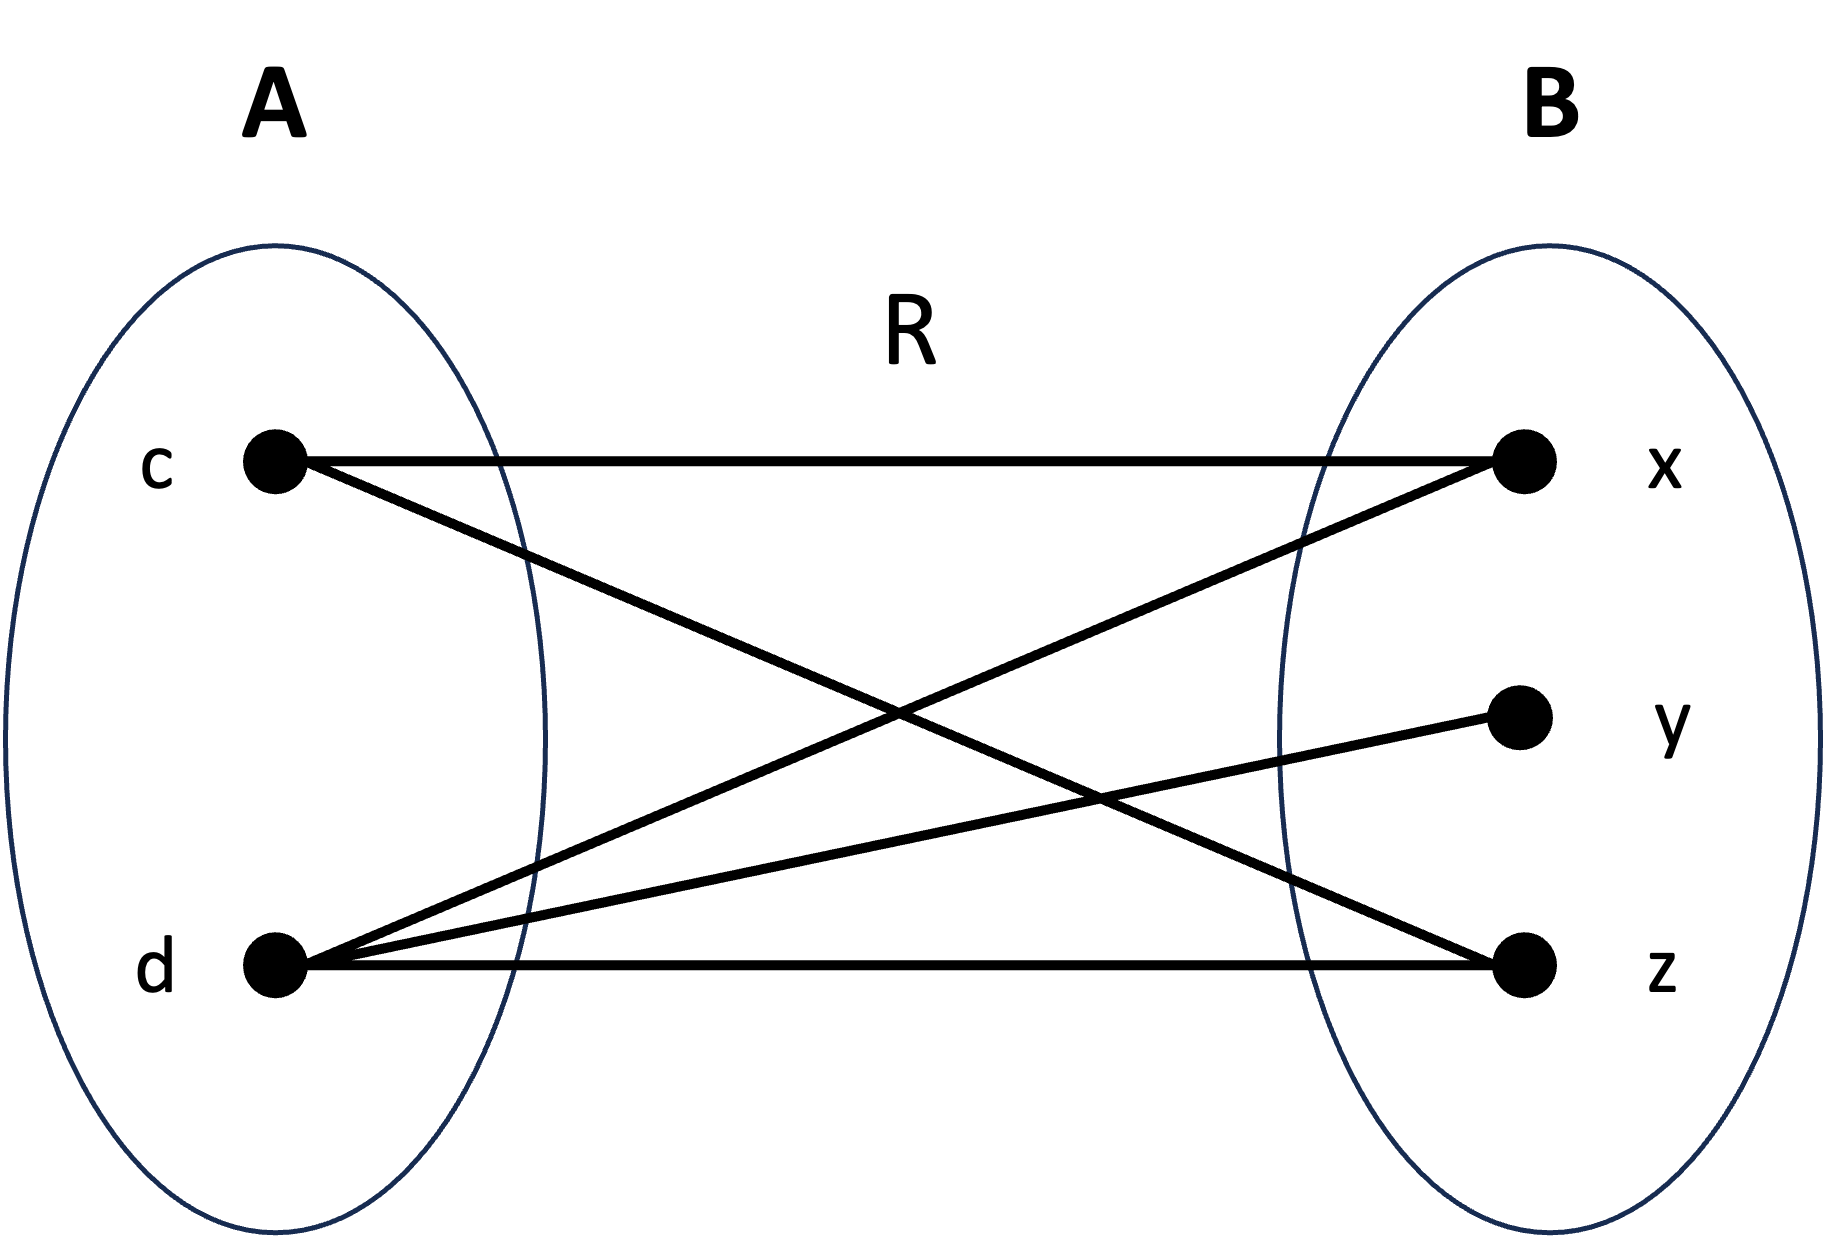
\includegraphics[scale=0.35]{../images/L1_Relations.png}
    \end{center}
\end{frame}

% Slide 16
\begin{frame}
    \frametitle{Types in Z Specification}
    \begin{itemize}
        \item Z specification language is \textbf{strongly typed}.
        \item Every expression is given a type.
        \item Any set can be used as a type.
        \item The following are equivalent declarations of variables $x$ and $y$ of types $A$ and $B$ respectively. 
        \begin{itemize}
            \item $(x, y) : A \cross B$
            \item $x: A, y: B$
            \item $x, y : A$ (only when $B = A$)
        \end{itemize}
    \end{itemize}
\end{frame}

% Slide 17
\begin{frame}[fragile]
\frametitle{Modelling using Z Specification}
\begin{itemize}
\item When we write a program, we can write code procedurally, functionally or in an object oriented manner.
\item Z Specification can help us model our code using two distinct sections.
\begin{enumerate}
    \item Declaration: To define variables.
    \item Predicate: Often used to define behaviours or invariants.
\end{enumerate}
\item \textbf{Example \#1:} We can define the relation \textbf{divides} between two natural numbers.

\texttt{| divides: $\nat_1 \rel \nat$ \\
| ----------------------------------------- \\
| $\forall x : \nat_1; y: \nat \spot x$ \underline{divides} $y \iff \exists k : \nat \spot x \cdot k = y$}

Usage: 3 \underline{divides} 6, $\lnot$ (3 \underline{divides} 7)

\item \textbf{Example \#2:} We can define the relation $\leq$ between two natural numbers.

\texttt{| $\_<=\_$: $\nat \rel \nat$ \\
| ----------------------------------------- \\
| $\forall x, y: \nat \spot x <= y \iff \exists k : \nat \spot x + k = y$}

The relation $<=$ is the infinite subset of ordered pairs in $\nat\cross\nat$.
\\$\{(0, 0), (0, 1), (1, 1), (0, 2) (1, 2), (2, 2), \ldots \}$
\end{itemize}
\end{frame}

% Slide 18
\begin{frame}{Domain and Range Restriction}
\begin{itemize}
    \item Let $A, B, R, S, T$ be sets.
    \item $A$ is the domain set, $B$ is the range set and $R$ is the relation set.
    \item Note that $S$ is a subset of the domain set and $T$ is the subset of the range set.
    \item Suppose $R: A \rel B, S \subseteq A$ and $T \subseteq B$.
    \begin{itemize}
        \item \textbf{Domain Restriction:} $S \dres R$ is the set $\{(a, b): R \mid a \in S\}$
        \item \textbf{Range Restriction:} $R \rres T$ is the set $\{(a, b): R \mid b \in T\}$
    \end{itemize}
    \item Notice that both $S \dres R \in A \rel B$ and $R \rres T \in A \rel B$, meaning that both domain restriction and range restrictions are relations from sets $A$ to $B$.
    \item If has\_sibling: People $\rel$ People then
    \begin{itemize}
        \item female $\dres$ has\_sibling is the relationship is\_sister\_of.
        \item has\_sibling $\rres$ female is the relationship has\_sister.
    \end{itemize}
\end{itemize}
\end{frame}

% Slide 19
\begin{frame}{Domain and Range Subtraction}
\begin{itemize}
    \item Let $A, B, R, S, T$ be sets.
    \item $A$ is the domain set, $B$ is the range set and $R$ is the relation set.
    \item Note that $S$ is a subset of the domain set and $T$ is the subset of the range set.
    \item Suppose $R: A \rel B, S \subseteq A$ and $T \subseteq B$.
    \begin{itemize}
        \item \textbf{Domain Subtraction:} $S \lefttrianglebar R$ is the set $\{(a, b): R \mid a \not \in S\}$
        \item \textbf{Range Subtraction:} $R \righttrianglebar T$ is the set $\{(a, b): R \mid b \not \in T\}$
    \end{itemize}
    \item The following predicates are true.
    \begin{itemize}
        \item $S \lefttrianglebar R = (A - S) \dres R$
        \item $R \righttrianglebar T = R \rres (B - T)$
        \item $S \lefttrianglebar R \in A \rel B$
        \item $R \righttrianglebar T \in A \rel B$
    \end{itemize}
    \item If has\_sibling: People $\rel$ People then
    \begin{itemize}
        \item female $\lefttrianglebar$ has\_sibling is the relationship is\_brother\_of.
        \item has\_sibling $\righttrianglebar$ female is the relationship has\_brother.
    \end{itemize}
\end{itemize}
\end{frame}

% Slide 20
\begin{frame}{Relational Image}
\begin{itemize}
    \item Suppose the relation $R : A \rel B$ and $S \rel A$
    \item $R \limg S \rimg = \{b : B \mid \exists a : S \spot a R b\}$
    \item $R \limg S \rimg \rel B$
    \item Example
    \begin{itemize}
        \item $divides \limg \{8, 9\} \rimg = \{x : \nat \mid \exists k : \nat \spot x = 8 \cdot k \vee 9 \cdot k \} = \{0, 8, 9, 16, 18, \ldots\}$
        \item $<= \limg {3, 7, 21} \rimg = \{x : \nat \mid x >= 3\}$ 
    \end{itemize}
    \item In summary, the relational image returns the set of all elements $b \in B$ such that there exists an $a \in S$ with $(a, b) \in R$.
    \item The difference between relational image and range restriction is that range restriction returns the subset of $R$ which are ordered pairs of $(a, b)$ where $a \in A$ and $b \in B$ and the first element $a$ of the ordered pair is in $S$. The relational image simply just returns the set of all second elements $b$.
\end{itemize}
\end{frame}

% Slide 21
\begin{frame}{Inverse and Relational Composition}
    \begin{itemize}
        \item \textbf{Inverse:} $R^{-1}$ is the set $\{(b, a) : B \cross A \mid a R b \}$ or $R^{-1} \in B \rel A$
        \begin{itemize}
            \item $has\_sibling^{-1} = has\_sibling$ 
            \item $divisor^{-1} = has\_divisor$ 
        \end{itemize}
        \item Example: $succ^{-1}$ = pred
        \\ \texttt{| succ: $\nat \rel \nat$
        \\|--------------------------------------
        \\| $\forall x, y : \nat \spot x$ \underline{succ} $y \rel x + 1 = y$ 
        }
    \end{itemize}
    \begin{columns}
        \begin{column}{0.65\textwidth}
            \begin{itemize}
                \item \textbf{Relational Composition ($\comp$)}
                \begin{itemize}
                    \item Suppose $R: A \rel B$ and $S: B \rel C$ are two relations.
                    \item $R \comp S = \{(a, c) : A \cross C \mid \exists b : B \mid a R b \wedge b S c\}$
                    \item $R \comp S \in A \rel C$
                \end{itemize}
                \item Examples
                \begin{itemize}
                    \item $is\_parent\_of \comp is\_parent\_of = is\_grandparent\_of$
                    \item $R^{0} = id[A]$, $R^{1} = R$ 
                    \item $R^{2} = R \comp R$
                    \item $R^{3} = R \comp R \comp R$
                \end{itemize}
            \end{itemize}   
        \end{column}
        \begin{column}{0.35\textwidth}
            \begin{center}
                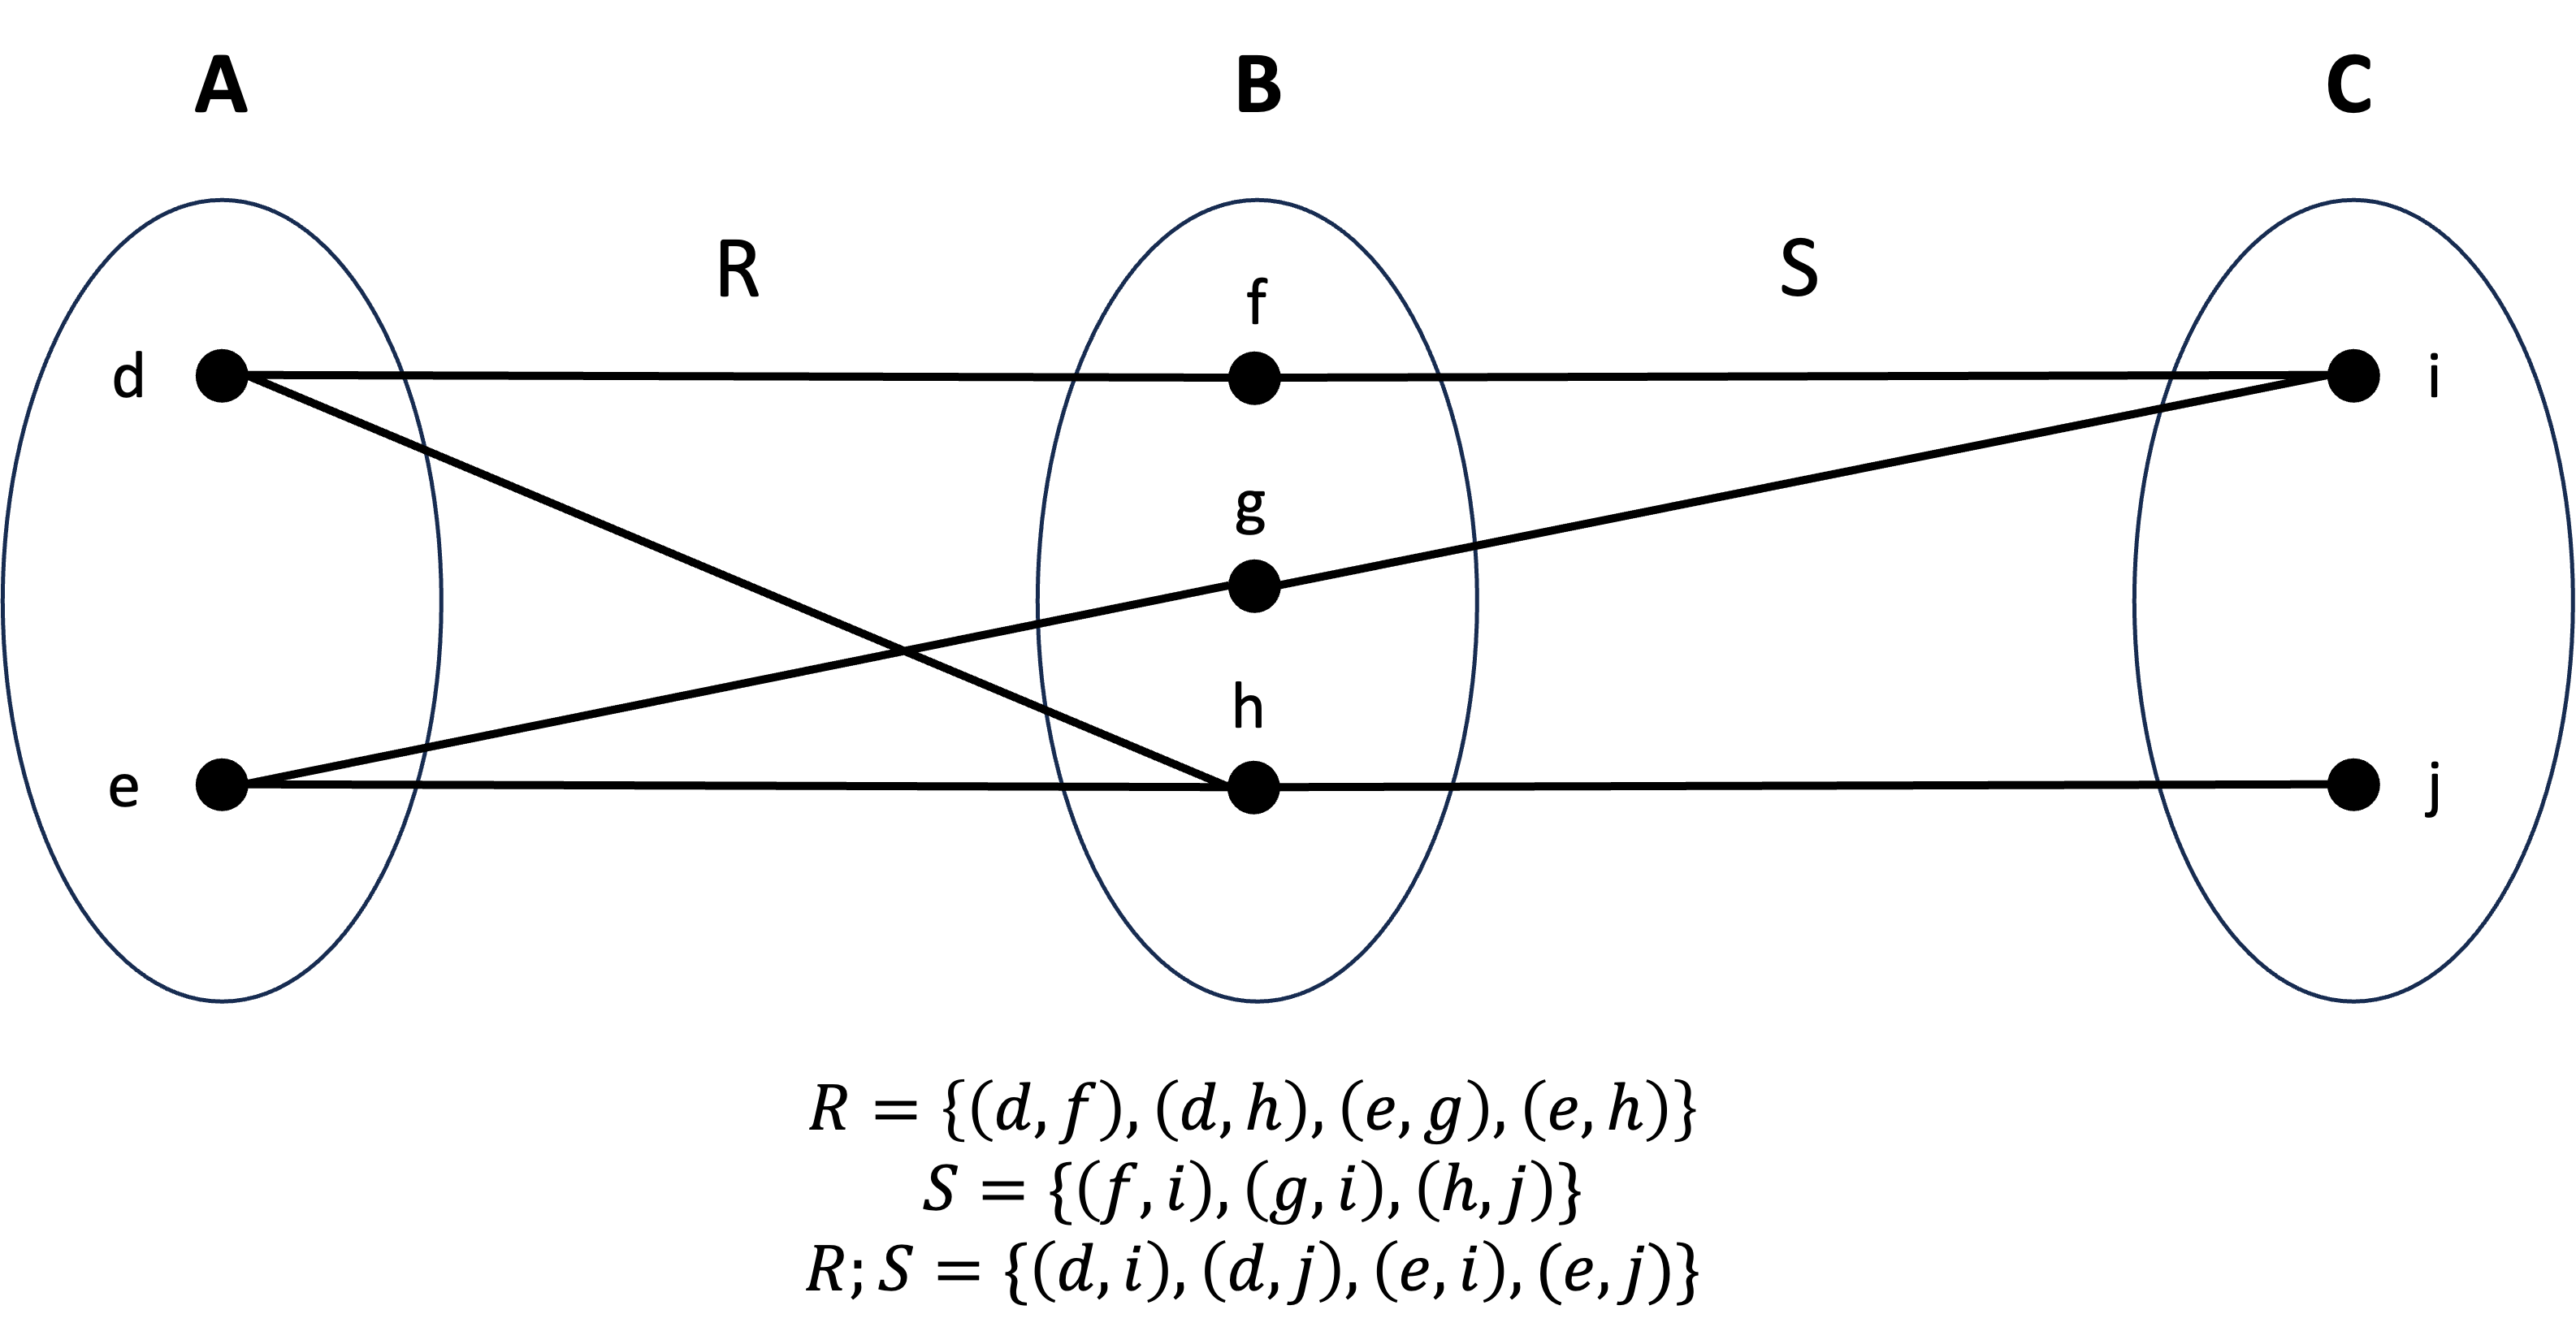
\includegraphics[scale=0.225]{../images/L1_RelationalComposition.png}
            \end{center}
        \end{column}
    \end{columns}
\end{frame}

% Slide 22
\begin{frame}{Recap on Functions}
    \begin{itemize}
        \item A (partial) function from a set $A$ to a set $B$, denoted by $f: A \pfun B$ is a subset $f$ of $A \cross B$ with the property that for each $a \in A$, there is \textbf{at most one} $b \in B$ with $(a, b) \in f$.
        \item \textbf{$\dom f$} is the set $\{a : A \mid \exists b : B \spot (a, b) \in f\}$
        \item \textbf{$\ran f$} is the set $\{b : B \mid \exists a : A \spot (a, b) \in f\}$
        \item Suppose $f: A \pfun B$ and $a \in \dom f$, then $f(a)$ denotes the unique image $b \in B$ that $a$ is mapped to by $f$.
        \item $(a, b) \in f$ is equivalent to $f(a) = b$
        \item \textbf{Total Function:} If the function $f: A \pfun B$ is a total function, then $f: A \rightarrow B$ if and only if $\dom f = A$
    \end{itemize}
    \begin{columns}
        \begin{column}{0.5\textwidth}
            \begin{center}
                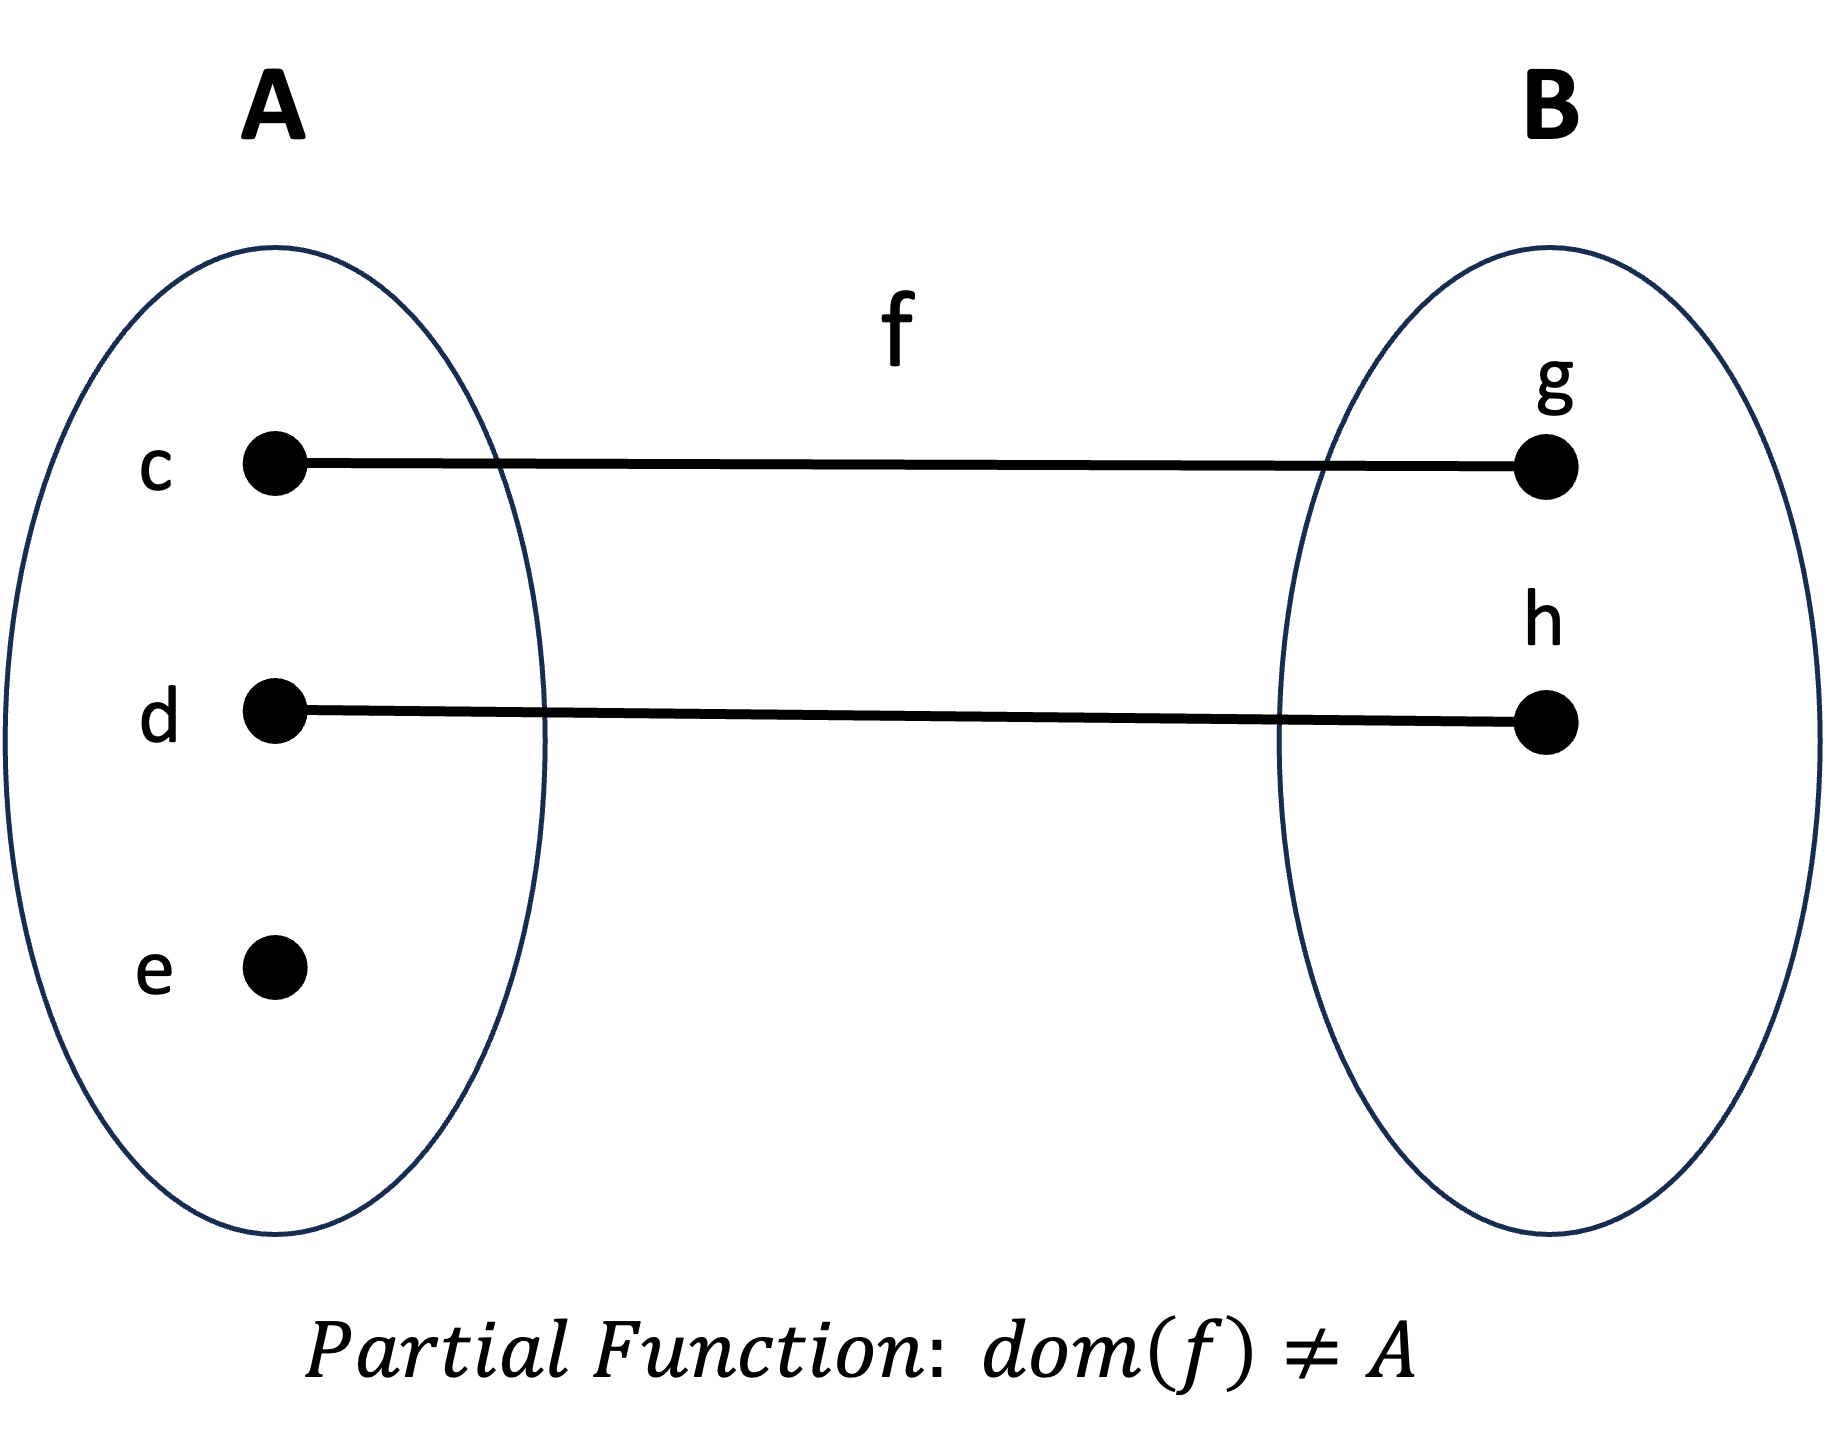
\includegraphics[scale=0.25]{../images/L1_PartialFunction.png}
            \end{center}
        \end{column}
        \begin{column}{0.5\textwidth}
            \begin{center}
                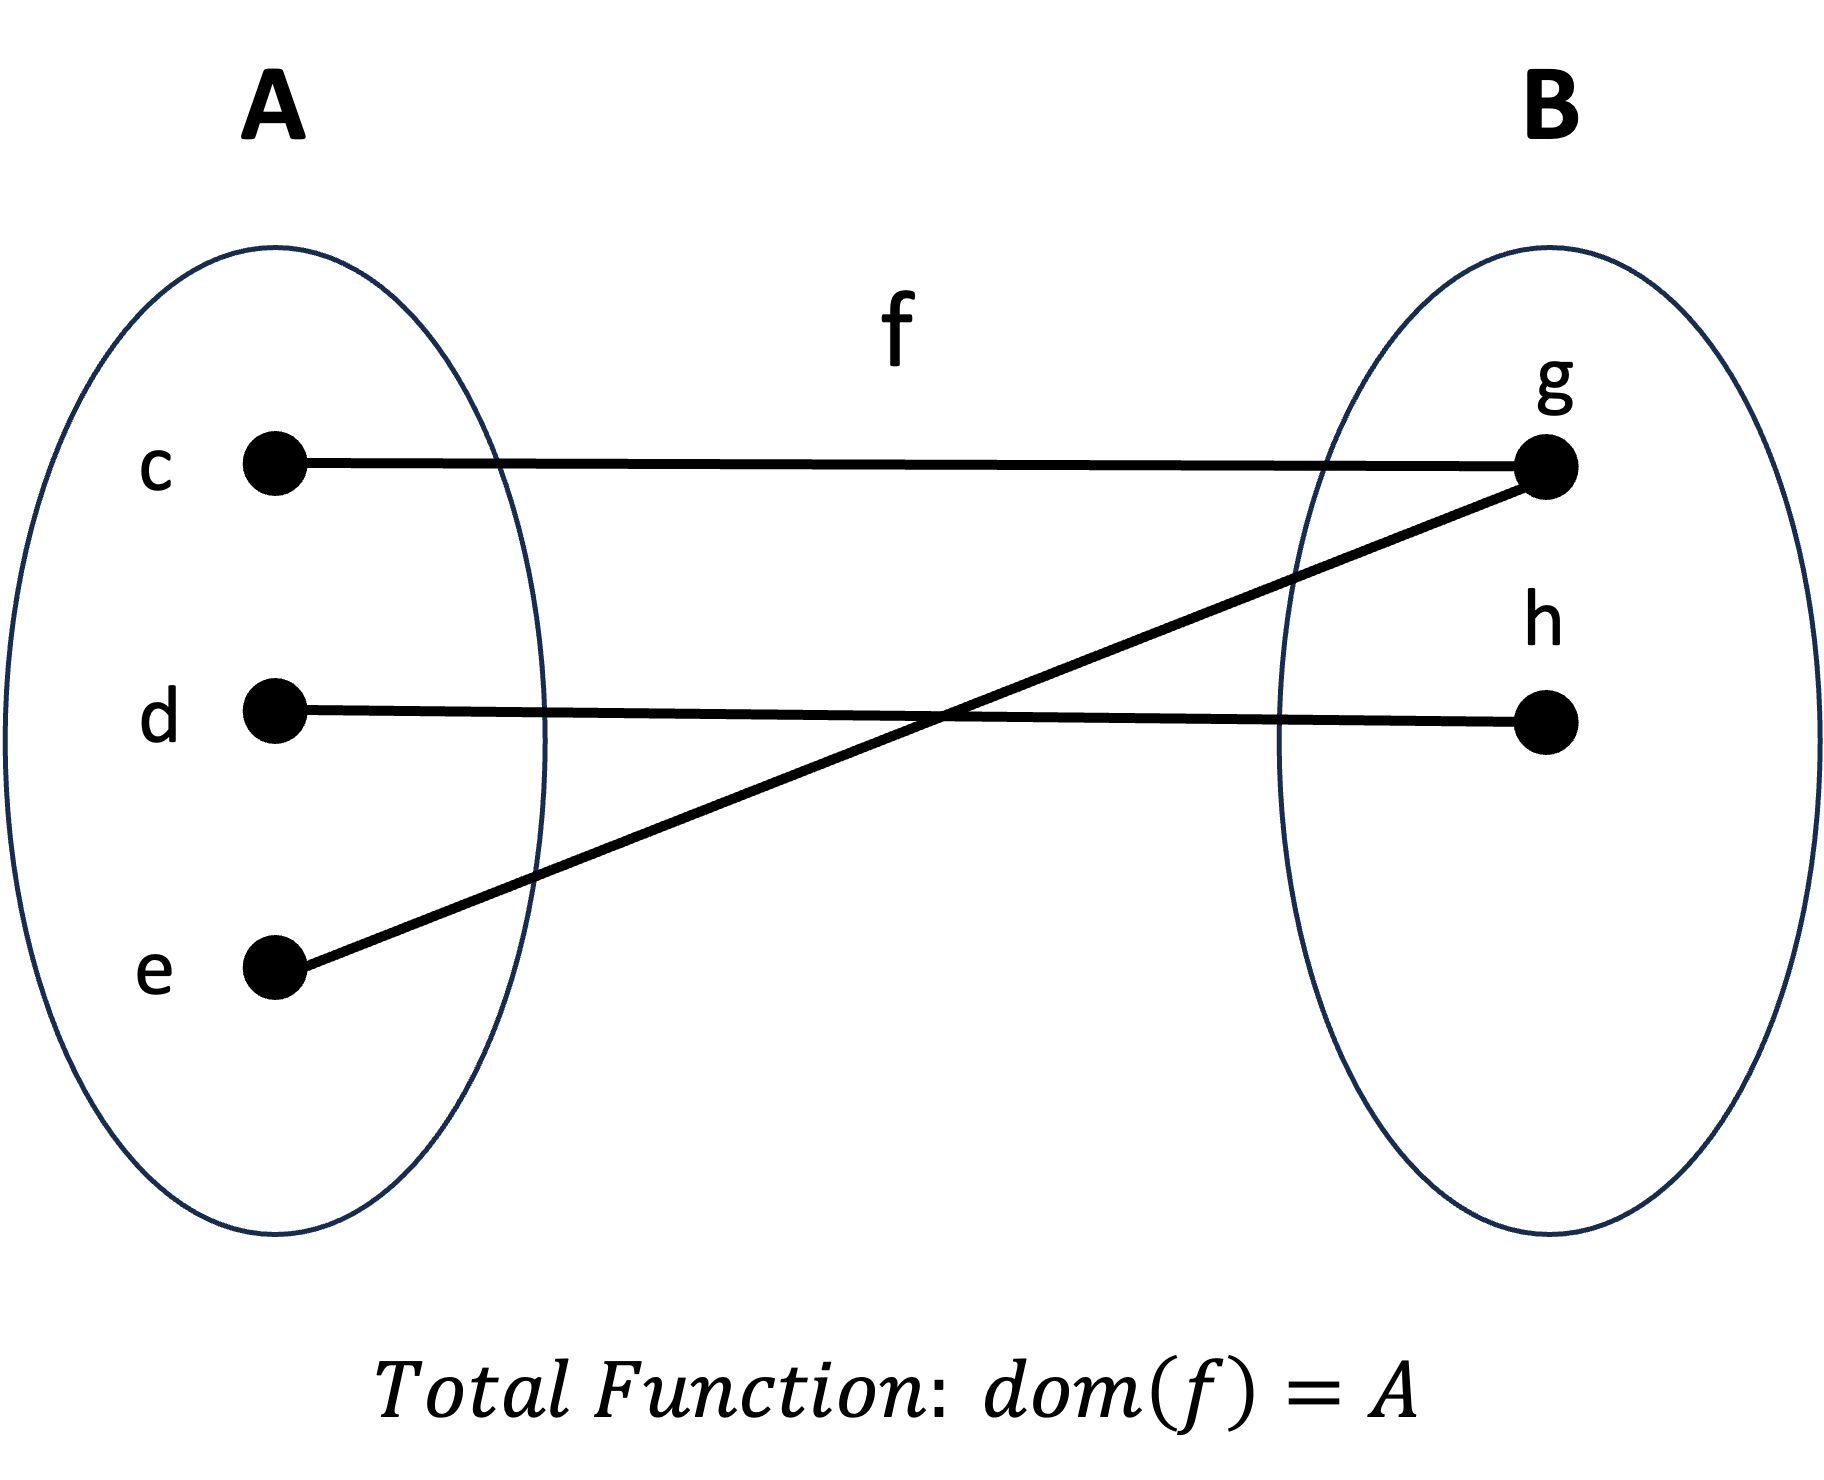
\includegraphics[scale=0.25]{../images/L1_TotalFunction.png}
            \end{center}
        \end{column}
    \end{columns}
\end{frame}

% Slide 23
\begin{frame}{Function Overriding}
    \begin{itemize}
        \item Suppose $f, g: A \pfun B$, then $f \oplus g$ is the function $(\dom g \lefttrianglebar f) \cup g$.
        \item The following predicates are true:
        \begin{enumerate}
            \item $\dom f \oplus g = \dom f \cup \dom g$
            \item $a : \dom g$ $\spot (f \oplus g)(a) = g(a)$
            \item $\forall a : \dom f - \dom g \spot (f \oplus g)(a) = f(a)$
            \item f $\oplus$ g $\in a \pfun b$
        \end{enumerate}
        \item Examples
        \begin{enumerate}
            \item $\{a \rightarrow x, b \rightarrow y, c \rightarrow x\} \oplus \{a \rightarrow y\} = \{a \rightarrow y, b \rightarrow y, c \rightarrow x\}$
            \item double $\oplus$ root = $\{(0, 0), (1, 1), (2, 4), (3, 6), (4, 2), \ldots\}$ (Note: $(4, 8)$ was replaced with $(4, 2)$ as the domain 4 is both in $f$ and $g$, so the range was replaced with $2$ that was in $g$)
        \end{enumerate}
    \end{itemize}
\end{frame}

% Slide 24
\begin{frame}
    \frametitle{Specifying Functions}
    \begin{enumerate}
        \item Using a look-up table
        \begin{itemize}
            \item If a function $f : A \pfun B$ is finite (and not too large), we can specify the function explicity by listing all pairs $(a, b)$ in the subset $A \cross B$.
            \item Example: PassportNo $\fun$ Address
            
            \begin{tabular}{c c}
                PassportNo & Address \\
                A001017 & 77 Sunset Strip \\
                $\cdots$ & $\cdots$ \\
                G707165 & 19 Mail Street
            \end{tabular}
        \end{itemize}

        \item Declaring Axioms: A function can be specified by giving a \textbf{predicate} determining which pairs $(a, b)$ are in the function.
        \begin{itemize}
            \item \textbf{Example: The root function that calculates the square root of a natural number} 
            
            \texttt{| root $\nat \pfun \nat$
            \\|--------------------------------
            \\| $\dom root = \{n : \nat \mid \exists m:\nat \spot m^{2} = n\}$
            \\| $\forall n : \dom root$ $\spot$ $(root(n))^{2} = n$}

        \end{itemize}
    \end{enumerate}
\end{frame}

% Slide 25
\begin{frame}[fragile]
    \frametitle{Specifying Functions}
    \begin{enumerate}
        \setcounter{enumi}{2}
        \item Using Recursion: For functions defined recursively in terms of itself.
        
        \texttt{| fact $\nat_1 \pfun \nat$
        \\|--------------------------------
        \\| fact(1) = 1
        \\| $\forall n : \nat_1 - \{1\} \spot fact(n) = n * fact(n - 1)$}

        \item Giving an Algorithm: A function $f : A \pfun B$ is specified by an algorithm such that given any element $a$ in the domain of $f$, the element $f(a)$ can be computed using the algorithm.
        \begin{columns}
            \begin{column}{0.4\textwidth}
\begin{lstlisting}
input n : N
var x, y: integer;
begin
    x := n; y:= 0;
    while x != 0 do
    begin
        x := x - 1; y:= y + 2
    end;
write(y)
end
\end{lstlisting}
            \end{column}
            \begin{column}{0.4\textwidth}  %%<--- here
                \texttt{| double: $\nat \fun \nat$\\
                | ------------------\\
                | $\forall n : \nat \spot double(n) = 2n$}
            \end{column}
        \end{columns}
    \end{enumerate}
\end{frame}

% Slide 26
\begin{frame}{Sequences}
    \begin{itemize}
        \item A sequence s of elements of a set $A$, denoted $s : \seq A$, is a function $s:\nat \pfun A$ where $\dom s = 1 \upto n$ for some natural number $n$.
        \item \textbf{Example}
        \begin{itemize}
            \item $<b, c, a, b>$ denotes the sequence (function) $\{1 \fun b, 2 \fun c, 3 \fun a, 4 \fun b\}$
            \item The empty sequence is denoted by $<>$
        \end{itemize}
        \item The set of all sequences of elements from $A$ is denoted as $\seq A$ and is defined to be $\seq A = \{s : \nat \pfun A \mid \exists n:\nat$ $\spot$ $\dom s = 1 \upto n\}$
        \item $\seq_1 A = \seq A - \{<>\}$ is defined as the set of non-empty sequences.
        \item Since sequences are ordered mapping, $<a, b, a> \neq <a, a, b> \neq <a, b>$
    \end{itemize}
\end{frame}

% Slide 27
\begin{frame}{Special Functions for Sequence}
    \begin{enumerate}
        \item Concatenation 
        \begin{itemize}
            \item $<a, b> \cat <b, a, c> = <a, b, b, a, c>$
        \end{itemize}
        \item Head
        \begin{itemize}
            \item \texttt{| head: $\seq_1 A \fun A$
            \\|---------------------------------
            \\|$\forall s : \seq_1 A \spot head(s) = s(1)$}
            \item $head<c, b, b> = c$
        \end{itemize}
        \item Tail
        \begin{itemize}
            \item \texttt{| tail: $\seq_1 A \fun \seq A$
            \\|---------------------------------
            \\|$\forall s : \seq_1 A \spot <head(s)>$ $\cat$ $tail(s) = s$}
            \item $tail<c, b, b> = <b, b>$
        \end{itemize}
        \item Filter
        \begin{itemize}
            \item $<a, b, c, d, e, d, c, b, a> \filter \{a, d\} = <a, d, d, a>$
            \item Filter only keeps the element in the specified set, preserves order in the original sequence and outputs a new sequence.
        \end{itemize}
        
    \end{enumerate}
\end{frame}

% Slide 28
\begin{frame}{Z Specification}
\begin{itemize}
\item As explained in an earlier slide, we can write Z Specification to formally specify requirements in \textbf{two distinct sections}
\begin{enumerate}
    \item Declaration: To define variables.
    \item Predicate: Often used to restrain the possible values of the declared variables to define behaviours or invariants.
\end{enumerate}
\item Formal Specification can be done in the form of both \textbf{axioms} and \textbf{schemas}.
\item When we were specifying functions earlier, we were formally specifying them in the form of \textbf{axioms} in the \textbf{axiom environment}.
\item Later we will introduce how to formally specify \textbf{schemas} which are used to specify relationships between variable values.
\item There are two main type of schemas in the \textbf{schema environment}
\begin{itemize}
    \item State Schema
    \item Operation Schema
\end{itemize}
\end{itemize}
\end{frame}

% Slide 29
\begin{frame}[fragile]
\frametitle{The \texttt{zed-csp} Package}
\begin{itemize}
    \item We can use the \texttt{zed-csp} package to formally specify requirements in Z Specification and render axioms and schemas them in TeX.
    \item There are \textbf{two types of environment} in the \texttt{zed-csp} package.
\end{itemize}
\begin{enumerate}
\item Axiom Environment

\begin{columns}
\begin{column}{0.4\textwidth}
\begin{small}
\begin{axdef}
limit: \nat
\where
limit \leq 65535
\end{axdef}
\end{small}
\end{column}
\begin{column}{0.6\textwidth}
\begin{lstlisting}
\begin{axdef}
    limit: \nat
    \where
    limit \leq 65535
\end{axdef}
\end{lstlisting} 
\end{column}
\end{columns}

\item Schema Environment
\begin{columns}
\begin{column}{0.4\textwidth}
\begin{small}
\begin{schema}{PhoneDB}
known: \power NAME \\ phone: NAME \pfun PHONE
\where
known = \dom phone
\end{schema}
\end{small}
\end{column}
\begin{column}{0.6\textwidth}
\begin{lstlisting}
\begin{schema}{PhoneDB}
known: \power NAME \\ phone: NAME \pfun PHONE
\where
known = \dom phone    
\end{schema}
\end{lstlisting}
\end{column}
\end{columns}
\end{enumerate}
\end{frame}

% Slide 30
\begin{frame}{State Schema}
    \begin{itemize}
        \item A \textbf{state schema} specifies a relationship between variable values
        \item It specifies a \underline{snapshot} of a system
        \item \textbf{Variables} are declared and typed in the \textbf{top part of the schema}.
        \item A \textbf{predicate (axiom)} restraining the possible values of the declared variables are given in the \textbf{bottom part of the schema.}
        \item An instance of a schema is an assignment of values to variables consistent with their type declaration and satisfying the predicate.
    \end{itemize}
\end{frame}

% Slide 31
\begin{frame}{Operation Schema}
    \begin{itemize}
        \item The state schema provides a static view of the system.
        \item To specify how the system can change, we need to specify the operation schema.
        \item An operation can be thought as taking an instance of the state schema and producing a new instance.
        \item To specify such an operation, we express as a predicate the relationship between the \textbf{instance of the state before the operation} and the \textbf{instance after the operation.}
        \begin{block}{Convention}
            \begin{itemize}
                \item The value of the state variables before the operation are denoted by \textbf{unprimed identifiers}.
                \begin{itemize}
                    \item Example: \texttt{items : seq MSG}
                \end{itemize}
                \item Values after the operation are denoted by \textbf{primed identifiers}.
                \begin{itemize}
                    \item Example: \texttt{items' : seq MSG}
                \end{itemize}
                \item Note: Let \texttt{MSG} be the set of all possible messages that can be transmitted.
            \end{itemize}
        \end{block}
    \end{itemize}
\end{frame}

% Slide 32
\begin{frame}{Case Study: A Message Buffer}
    \begin{itemize}
        \item We are going to model a message buffer to learn about \textbf{schema specification}.
        \item A message buffer stores messages within a queue data structure and operates on a first in / first out (FIFO) principle.
        \item Suppose we have a line which might be occupied by traffic, many messages join the buffer and but only the first message in the queue leaves the buffer when the line is free.
        \item The buffer may contain several messages at any time, but there is a fixed upper limit on the number of messages the buffer may contain.
        \item To model a message buffer, we minimally need the following:
        \begin{enumerate}
            \item States: Buffer (to store messages)
            \item Operations: Join (new message joins the buffer), Leave (message leaves the buffer)
        \end{enumerate}
    \end{itemize}
    \begin{center}
        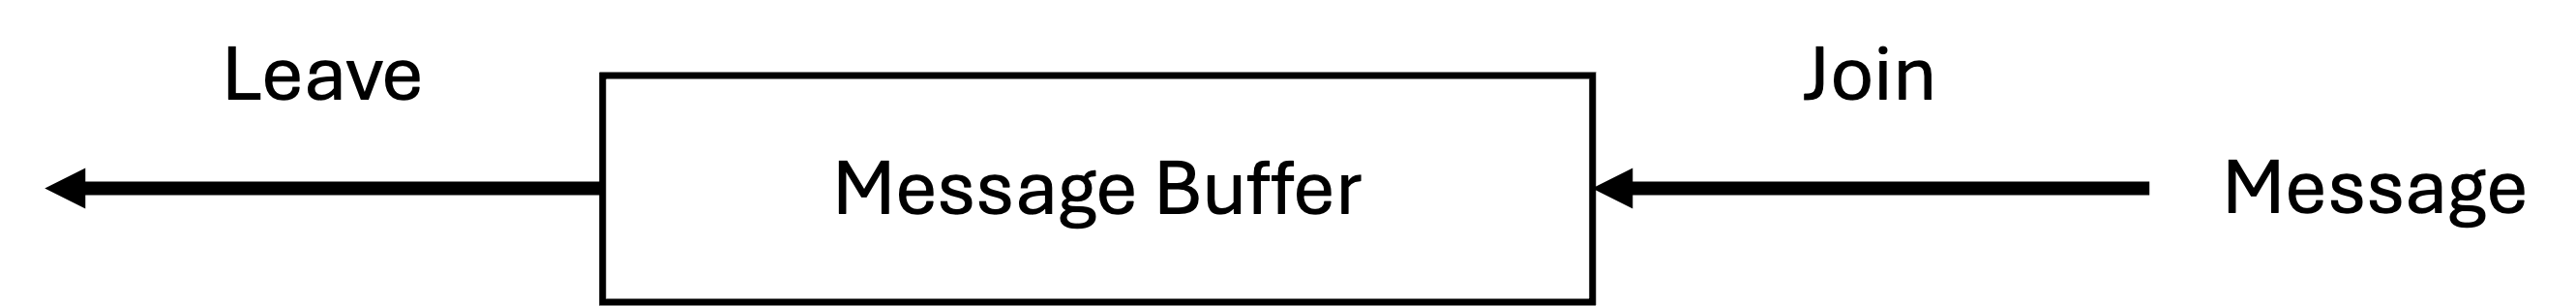
\includegraphics[scale=0.5]{../images/MessageBuffer.png}
    \end{center}
\end{frame}

% Slide 33
\begin{frame}{Formal Specification: Message Buffer}
\begin{columns}
\begin{column}{0.6\textwidth}
\textbf{State Schema: Buffer}
\begin{itemize}
    \item Let MSG be the set of all possible messages that can be transmitted.
    \item Let max : $\nat$ be the constant maximum number of messages that can be held in the buffer at any one time.
    \item Example: Let $MSG=\{m1, m2, m3\}$ and $max = 4$
    \begin{enumerate}
        \item $items = <m1, m2>$ is a valid instance.
        \item $items = <m3, m1, m1, m2, m2>$ is an invalid instance.
    \end{enumerate}
\end{itemize}
\textbf{Operation Schema: Join} 
\begin{itemize}
    \item The decoration ? denotes an input
    \item There is an implicit $\wedge$ between each line in the predicate section.
\end{itemize}
\end{column}
\begin{column}{0.4\textwidth}
\begin{small}
\begin{schema}{Buffer}
    items: \seq MSG
    \where
    \#items \leq max
\end{schema} 

\begin{schema}{Join}
    items, items': \seq MSG \\
    msg?: MSG
    \where
    \#items \leq max \\
    \#items' \leq max \\
    \#items < max \\
    items' = items \cat <msg?>
\end{schema}
\end{small}
\end{column}
\end{columns}
\end{frame}

% Slide 34
\begin{frame}{Explanation: Predicate of the Join Operation}
    \begin{columns}
        \begin{column}{0.4\textwidth}
            \begin{small}
                \begin{schema}{Join}
                    items, items': \seq MSG \\
                    msg?: MSG
                    \where
                    \#items \leq max \\
                    \#items' \leq max \\
                    \#items < max \\
                    items' = items \cat <msg?>
                \end{schema}
            \end{small}
        \end{column}
        \begin{column}{0.6\textwidth}
            \begin{itemize}
                \item The first two lines of the predicate indicate that we have a valid instance of the state schema \textbf{Buffer} both before and after the operation.
                \item The third line of the predicate is a pre-condition for the operation. It indicates that for the \textbf{Join} operation to be possible, the buffer must not be completely full.
                \item The last line of the predicate specifies the relationship between the buffer contents before and after the operation which is that the input message is already appended to the sequence of messages already in the buffer.
            \end{itemize}
        \end{column}
    \end{columns}
\end{frame}

% Slide 35
\begin{frame}{Formal Specification: Message Buffer (Continued)}
    \begin{columns}
        \begin{column}{0.63\textwidth}
            \textbf{Operation Schema: Leave}
            \begin{itemize}
                \item The decoration ! denotes an output
                \item There is an implicit $\wedge$ between each line in the predicate section.
                \item Explanation for Leave Operation Predicate
                \begin{enumerate}
                    \item The first two lines of the predicate indicate that we have a valid instance of the state schema \textbf{Buffer} both before and after the operation.
                    \item The third line of the predicate is a \textbf{pre-condition} for the operation. It indicates that for the \textbf{Leave} operation to be possible, the buffer must not be empty.
                    \item The last line of the predicate specifies the relationship between the buffer contents before and after the operation. The output message is taken from the head of the sequence of messages in the buffer, leaving just the tail of the sequence of buffers.
                \end{enumerate}
            \end{itemize}
        \end{column}
        \begin{column}{0.4\textwidth}
            \begin{schema}{Leave}
                items, items': \seq MSG \\
                msg!: MSG
                \where
                \#items \leq max \\
                \#items' \leq max \\
                \#items \neq \emptyset \\
                items = <msg!> \cat items'
            \end{schema}
        \end{column}
    \end{columns}
\end{frame}

% Slide 36
\begin{frame}{Special States: Delta ($\Delta$) and Initial State ($_{INIT}$)} 
\begin{enumerate}
\item Delta ($\Delta$): To specify a \textbf{before} and \textbf{after} instance of the state schema for any operation.
\begin{small}
\begin{schema}{\Delta Buffer}
    items, items': \seq MSG
    \where
    \#items \leq max\\
    \#items' \leq max
\end{schema} 
\end{small}
\item Initial State ($_{INIT}$): To specify a state when an instance of a state is first initialized.
\begin{columns}
    \begin{column}{0.25\textwidth}
        \begin{small}
            \begin{schema}{Buffer_{INIT}}
                Buffer
                \where
                items = <>
            \end{schema} 
            \end{small}
    \end{column}
    \begin{column}{0.75\textwidth}
        \begin{small}
            \begin{itemize}
                \item Initially the buffer would be empty.
                \item Then, the operations of \textbf{Join} and \textbf{Leave} can occur whenever they are enabled.
                \item Operations are assumed to be atomic.
                \item At all times, an observer will notice that the state schema is satisfied.
            \end{itemize}
        \end{small}
    \end{column}
\end{columns}
\end{enumerate}
\end{frame}

% Slide 37
\begin{frame}{Schema Inclusion}
\begin{itemize}
    \item Schema Inclusion is the act of including a schema in the declaration of another schema.
    \item It means the included schema has its declaration added to the new schema, and its predicate cojoined to the predicate of the new schema.
    \item The first "S" Schema is the \textbf{short form}, while the second "S" Schema is the \textbf{long form}.
\end{itemize}
\begin{columns}
    \begin{column}{0.33\textwidth}
        \begin{schema}{A}
            x: T_1\\
            y: T_2
            \where
            P(x, y)
        \end{schema}
    \end{column}
    \begin{column}{0.33\textwidth}
        \begin{schema}{S}
            A\\
            z: T_3
            \where
            Q(x, y, z)
        \end{schema}
    \end{column}
    \begin{column}{0.33\textwidth}
        \begin{schema}{S}
            x: T_1\\
            y: T_2\\
            z: T_3
            \where
            P(x, y) \wedge Q(x, y, z)
        \end{schema}
    \end{column}
\end{columns}
\end{frame}

% Slide 38
\begin{frame}{Example: Schema Inclusion}
    \begin{columns}
        \begin{column}{0.5\textwidth}
            \begin{schema}{Join}
                \Delta Buffer \\
                msg?: MSG
                \where
                \#items < max \\
                items' = items \cat <msg?>
            \end{schema}
        \end{column}
        \begin{column}{0.5\textwidth}
            \begin{schema}{Leave}
                \Delta Buffer \\
                msg!: MSG
                \where
                items \neq \emptyset \\
                items = <msg!> \cat items'
            \end{schema}
        \end{column}
    \end{columns}
    \begin{itemize}
        \item We can include the $\Delta Buffer$ schema to both the Join and Leave operations.
        \item Explanation for Leave Operation Predicate
        \begin{enumerate}
            \item The first line of the predicate is a \textbf{pre-condition} for the operation. It indicates that for the \textbf{Leave} operation to be possible, the buffer must not be empty.
            \item The last line of the predicate specifies the relationship between the buffer contents before and after the operation. The output message is taken from the head of the sequence of messages in the buffer, leaving just the tail of the sequence of buffers.
        \end{enumerate}
    \end{itemize}
\end{frame}

% Slide 39
\begin{frame}{Merging Schemas}
    \begin{itemize}
        \item \textbf{Type Compatability} is needed to merge schemas.
        \item In this case, the variable $y$ is common between states $A$ and $B$.
        \item We can simply merge the two types into a new state $C$ without further specifying any new predicates.
        \item The full form of state $C$ is also provided.
    \end{itemize}
    \begin{columns}
        \begin{column}{0.25\textwidth}
            \begin{schema}{A}
                x: T_1\\
                y: T_2
                \where
                P(x, y)
            \end{schema}
        \end{column}
        \begin{column}{0.25\textwidth}
            \begin{schema}{B}
                y: T_2\\
                z: T_3
                \where
                Q(y, z)
            \end{schema}
        \end{column}
        \begin{column}{0.2\textwidth}
            \begin{schema}{C}
                A\\
                B
            \end{schema}
        \end{column}
        \begin{column}{0.3\textwidth}
            \begin{schema}{C}
                x: T_1\\
                y: T_2\\
                z: T_3
                \where
                P(x, y) \wedge Q(y, z)
            \end{schema}
        \end{column}
    \end{columns}    
\end{frame}

% Slide 40
\begin{frame}{Extending Specifications: Slow Buffer and Slow Operations}
    \begin{itemize}
        \item Applying concepts such as \textbf{Schema Inclusion} and \textbf{Merging Schemas}, we can extend specifications similar to inheritance or creating specialized classes in Object-Oriented Programming. 
        \item To demonstrate this, we will attempt to model a \textbf{Slow Buffer} which has a constant $delay: \nat$ to simulate that each new message can only join the buffer after $delay$ seconds.
    \end{itemize}
    \begin{footnotesize}
        \begin{columns}
            \begin{column}{0.25\textwidth}
                \begin{schema}{SlowBuffer}
                    Buffer\\
                    idle: \nat
                \end{schema}

                \begin{schema}{Tick}
                    \Delta SlowBuffer\\
                    \where
                    idle' = idle + 1\\
                    items' = items
                \end{schema}
            \end{column}
            \begin{column}{0.25\textwidth}
                \begin{schema}{SlowBuffer_{INIT}}
                    SlowBuffer\\
                    Buffer_{INIT}
                    \where
                    idle = 0
                \end{schema}
            \end{column}
            \begin{column}{0.25\textwidth}
                \begin{schema}{SlowJoin}
                    \Delta SlowBuffer\\
                    Join
                    \where
                    idle \geq delay\\
                    idle' = 0
                \end{schema}
            \end{column}
            \begin{column}{0.25\textwidth}
                \begin{schema}{SlowLeave}
                    \Delta SlowBuffer\\
                    Leave \\
                    \where
                    idle \geq delay\\
                    idle' = 0
                \end{schema}
            \end{column}
        \end{columns} 
    \end{footnotesize}  
\end{frame}

% Slide 41
\begin{frame}{Extending Specifications: Slow Buffer and Slow Operations (Full Form)}
    \begin{footnotesize}
        \begin{columns}
            \begin{column}{0.25\textwidth}
                \begin{schema}{SlowBuffer}
                    items: \seq MSG\\
                    idle: \nat
                    \where
                    \#items \leq max
                \end{schema}
            \end{column}
            \begin{column}{0.25\textwidth}
                \begin{schema}{SlowBuffer_{INIT}}
                    items: \seq MSG\\
                    idle: \nat
                    \where
                    \#items \leq max\\
                    items = <>\\
                    idle = 0
                \end{schema}
            \end{column}
            \begin{column}{0.55\textwidth}
                \begin{schema}{SlowJoin}
                    items, items': \seq MSG\\
                    idle, idle': \nat
                    msg?: MSG
                    \where
                    \#items \leq max \wedge \#items' \leq max\\
                    \#items < max \wedge items' = items \cat <msg?>\\
                    idle \geq delay \wedge idle' = 0
                \end{schema}
            \end{column}
        \end{columns}
        \begin{columns}
            \begin{column}{0.5\textwidth}
                \begin{schema}{SlowLeave}
                    items, items': \seq MSG\\
                    idle, idle': \nat\\
                    msg!: MSG
                    \where
                    \#items \leq max \wedge \#items' \leq max\\
                    items \neq \emptyset \wedge items = items' \cat <msg?>\\
                    idle \geq delay \wedge idle' = 0
                \end{schema}
            \end{column}
            \begin{column}{0.5\textwidth}
                \begin{schema}{Tick}
                    items: \seq MSG\\
                    idle: \nat
                    \where
                    \#items \leq max \wedge \#items' \leq max\\
                    idle' = idle + 1 \wedge items' = item
                \end{schema}
            \end{column}
        \end{columns}
    \end{footnotesize}
\end{frame}

% Slide 42
\begin{frame}{Reasoning About The Specification}
    \begin{itemize}
        \item Suppose, we want to verify that message buffer specified has the \textbf{FIFO property}.
        \item We want to show that the messages leave the buffer in the same order they arrive.
        \item In this case, we introduce \textbf{auxillary sequences} \texttt{inhist} and \texttt{outhist} to record the history of the flow of messages into and out of the buffer.
        \item Create a new schema which includes the original Buffer and Operation schemas and extra information about the auxillary variables.
        \item When a message \textbf{joins} the buffer, it is also added to the \texttt{inhist} sequence.
        \item When a message \textbf{leaves} the buffer, it is added to the \texttt{outhist} sequence.
    \end{itemize}
\end{frame}

% Slide 43
\begin{frame}{Recorded Buffer and Operations}
    \begin{columns}
        \begin{column}{0.5\textwidth}
            \begin{schema}{RecordedBuffer}
                Buffer\\
                inhist: \seq MSG\\
                outhist: \seq MSG
            \end{schema}

            \begin{schema}{RecordedBuffer_{INIT}}
                RecordedBuffer\\
                Buffer_{INIT}
                \where
                inhist = <>\\
                outhist = <>
            \end{schema}
        \end{column}
        \begin{column}{0.5\textwidth}
            \begin{schema}{RecordedJoin}
                \Delta RecordedBuffer\\
                Join
                \where
                inhist' = inhist \cat <msg?>\\
                outhist' = outhist
            \end{schema}

            \begin{schema}{RecordedLeave}
                \Delta RecordedBuffer\\
                Join
                \where
                inhist' = inhist\\
                outhist' = outhist \cat <msg!>
            \end{schema}
        \end{column}
    \end{columns}
\end{frame}

% Slide 44
\begin{frame}{RecordedJoin: Expanded Schema}
    \begin{schema}{RecordedJoin}
        items, items': \seq MSG\\
        inhist, inhist': \seq MSG\\
        outhist, outhist': \seq MSG\\
        msg?: MSG
        \where
        \#items \leq max \wedge \#items' \leq max\\
        \#items < max \wedge items' = items \cat <msg?>\\
        inhist' = inhist \cat <msg?>
        outhist' = outhist
    \end{schema}
\end{frame}

% Slide 45
\begin{frame}{Proving the FIFO Property}
    \begin{itemize}
        \item How can we use the auxillary variables \texttt{inhist} and \texttt{outhist} to prove that the buffer satisifies the \textbf{FIFO property}?
        \item We can prove that the predicate $\forall RecordedBuffer \spot inhist = outhist \cat items$ is true.
        \item Prove using structural induction.
        \begin{enumerate}
            \item Initially \texttt{inhist = outhist = items = <>}, so the predicate is true for the initial state.
            \item Suppose the predicate is true, and RecordedJoin occurs. After the operation, $inhist' = inhist \cat <msg?> \wedge outhist' = outhist \wedge items' = items \cat <msg?>$
            \item Hence, $inhist \cat <msg?> = (outhist \cat items) \cat <msg?>$ $= outhist \cat (items \cat <msg?>) = outhist' \cat items'$ 
            \item Therefore, the predicate remains true.
        \end{enumerate}
        \item We can construct a similar argument that the operation \textbf{RecordedLeave} also preserves the predicate.
    \end{itemize}
\end{frame}

% Slide 46
\begin{frame}{Conjunction of Schemas}
    \begin{itemize}
        \item When using the conjunction ($\wedge$) operator on two schemas, it is equivalent to merging the two schemas.
        \item Suppose $A$ and $B$ are schemas
        \begin{itemize}
            \item The declaration of $A \wedge B$ is the \textbf{union} of the declarations of $A$ and $B$
            \item The predicate of $A \wedge B$ is the \textbf{conjunction} of the predicates of $A$ and $B$
        \end{itemize}
        \item Examples
        \begin{enumerate}
            \item $SlowRecordedBuffer \defs SlowBuffer \wedge RecordedBuffer$
            \item $SlowRecordedBuffer_{INIT} \defs SlowBuffer_{INIT} \wedge RecordedBuffer_{INIT}$
            \item $SlowRecordedJoin \defs SlowJoin \wedge RecordedJoin$
        \end{enumerate}
        \item SlowRecordedBuffer Schema
        \begin{schema}{SlowRecordedBuffer}
            SlowBuffer\\
            RecordedBuffer
        \end{schema}
    \end{itemize}
\end{frame}

% Slide 47
\begin{frame}{Disjunction of Schemas}
    \begin{itemize}
        \item Using the conjunction ($\wedge$) operator on two schemas yields a different result.
        \item Suppose $A$ and $B$ are schemas
        \begin{itemize}
            \item The declaration of $A \vee B$ is the \textbf{union} of the declarations of $A$ and $B$
            \item The predicate of $A \vee B$ is the \textbf{disjunction} of the predicates of $A$ and $B$
        \end{itemize}
    \end{itemize}
    \begin{columns}
        \begin{column}{0.2\textwidth}
            \begin{schema}{A}
                x: T_1\\
                y: T_2
                \where
                P(x, y)
            \end{schema}
        \end{column}
        \begin{column}{0.2\textwidth}
            \begin{schema}{B}
                y: T_2\\
                z: T_3
                \where
                Q(y, z)
            \end{schema}
        \end{column}
        \begin{column}{0.3\textwidth}
            \begin{schema}{A \wedge B}
                x: T_1\\
                y: T_2\\
                z: T_3
                \where
                P(x, y) \wedge Q(y, z)
            \end{schema}
        \end{column}
        \begin{column}{0.3\textwidth}
            \begin{schema}{A \vee B}
                x: T_1\\
                y: T_2\\
                z: T_3
                \where
                P(x, y) \vee Q(y, z)
            \end{schema}
        \end{column}
    \end{columns}
\end{frame}

% Slide 48
\begin{frame}{Disjunction of Schemas: Example}
    \begin{itemize}
        \item Let $Flag ::= ok \mid error$ (The Flag type can be either 'ok' or 'error')
        \item $\Xi$ State is another special state that is used for operations that access information in the state \textbf{without changing the state at all}.
        \item Example: $CompleteJoin \defs JoinOk \vee JoinError$
    \end{itemize}
    \begin{footnotesize}
        \begin{columns}
            \begin{column}{0.5\textwidth}
                \begin{schema}{JoinOk}
                    Join\\
                    flag!: Flag
                    \where
                    flag! = ok
                \end{schema}
            \end{column}
            \begin{column}{0.5\textwidth}
                \begin{schema}{JoinError}
                    \Xi Buffer\\
                    flag!: Flag
                    \where
                    \#items = max \wedge flag != error
                \end{schema}
            \end{column}
        \end{columns}
        \begin{schema}{CompleteJoin}
            \Delta Buffer\\
            msg?: MSG; flag!: Flag
            \where
            \#items < max \wedge items' = item \cat <msg?> \wedge flag! = ok\\
            \vee\\
            \#items = max \wedge items' = items \wedge flag! = error
        \end{schema}
    \end{footnotesize}
\end{frame}

% Slide 49
\begin{frame}{Composition of Schemas}
    \begin{itemize}
        \item Using the composition operator ($\comp$) on two schemas is typically used to combine the effects of two operations.
        \item Example: $JoinLeave = Join \comp Leave$
            \begin{itemize}
                \item The pre-state of $Join$ is the pre-state of $Join \comp Leave$.
                \item The post-state of $Join$ is identified with the pre-state of $Leave$ hidden within $Join \comp Leave$.
                \item The consequent post-state of $Leave$ is the post-state of $Join \comp Leave$.
            \end{itemize}
        \item Convention: Hidden state is denoted with double prime ('').
    \end{itemize}
    \begin{schema}{JoinLeave}
        \Delta Buffer\\
        msg?, msg!: MSG
        \where
        \#items < max\\
        \exists items'': \seq MSG \spot items'' = items \cat <msg?> \wedge items'' = <msg!> \cat items'
    \end{schema}
\end{frame}

% Slide 50
\begin{frame}{Composition of Schemas in general}
    \begin{columns}
        \begin{column}{0.2\textwidth}
            \begin{schema}{A}
                x: T_1\\
                y: T_2
                \where
                P(x, y)
            \end{schema}
        \end{column}
        \begin{column}{0.4\textwidth}
            \begin{schema}{AOP_{1}}
                \delta A\\
                t_{3}?: T_3; t_{4}!: T_4
                \where
                Q_{1}(x, x', y, y', t_{3}?, t_{4}!)
            \end{schema}
        \end{column}
        \begin{column}{0.4\textwidth}
            \begin{schema}{AOP_{2}}
                \delta A\\
                t_{5}?: T_5; t_{6}!: T_6
                \where
                Q_{2}(x, x', y, y', t_{5}?, t_{6}!)
            \end{schema}
        \end{column}
    \end{columns}
    \begin{schema}{AOP_{1} \comp AOP_{2}}
        \delta A\\
        t_{3}?: T_3; t_{4}!: T_4; t_{5}?: T_5; t_{6}!: T_6
        \where
        \exists x'': T_1; y'': T_2 \spot Q_{1}(x, x', y, y', t_{3}?, t_{4}!) \wedge Q_{2}(x, x', y, y', t_{5}?, t_{6}!)
    \end{schema}
\end{frame}

% Slide 51
\begin{frame}{Z Specification Case Study: Shunting Game}
    \begin{columns}
        \begin{column}{0.7\textwidth}
            \begin{itemize}
                \item The diagram illustrates the board and the starting state for a shunting game.
                \item The black piece is the shunter.
                \item A move consists of the black piece (the shunter) moving one position either vertically or horizontally provided either:
                \begin{itemize}
                    \item The position moved to is empty, or
                    \item The position moved to is occupied by a white piece but the position beyond the white piece is empty, in which case the white piece is pushed into the empty position.
                \end{itemize}
                \item The shunter cannot push two white pieces at the same time.
                \item At each stage, a score is kept of the number of moves made so far.
                \item The game ends when the white pieces occupy the four positions marked with a cross.
            \end{itemize}
        \end{column}
        \begin{column}{0.3\textwidth}
            \begin{center}
                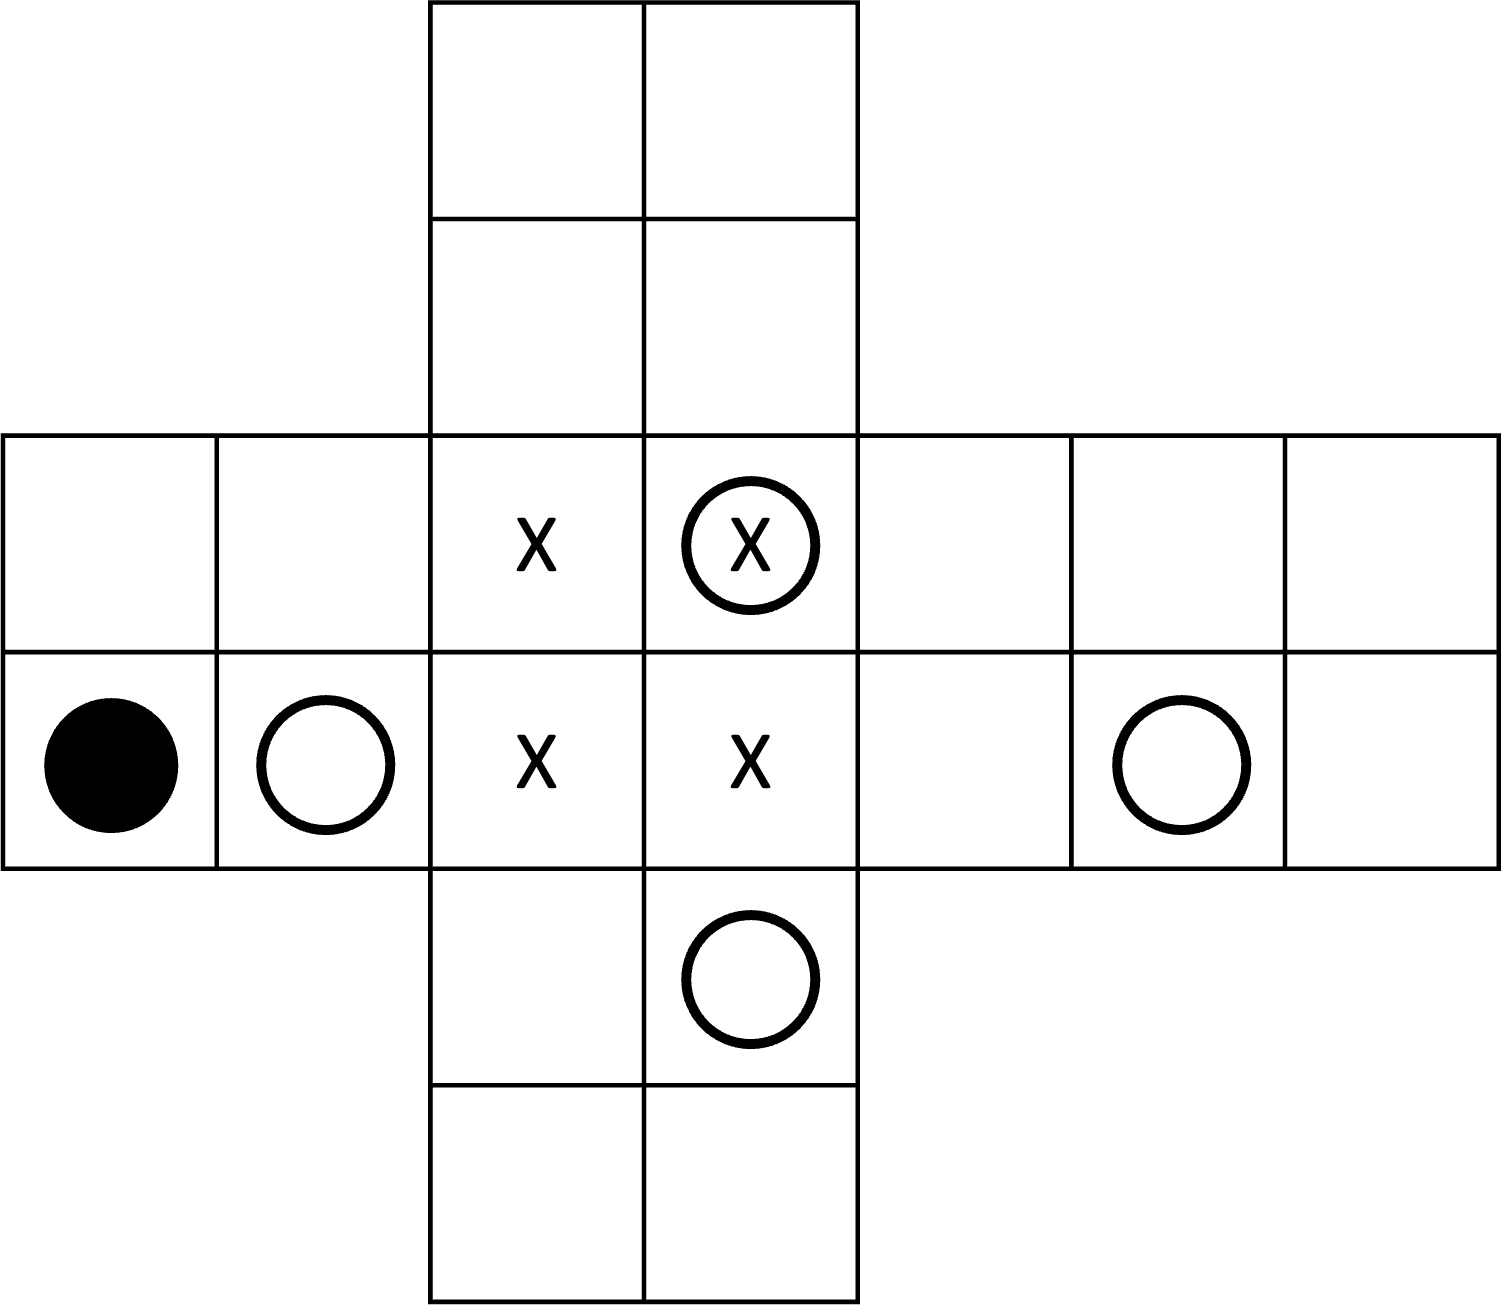
\includegraphics[scale=0.4]{../images/L1_ShuntingGame.png}
            \end{center}
        \end{column}
    \end{columns}
\end{frame}

% Slide 52
\begin{frame}{Z Specification Case Study: Shunting Game (Writing the Specification)}
    \begin{itemize}
        \item $Board == (1..7 \cross 3..4) \cup (3..4 \cross 1..6)$
        \item $over == \set{(3, 3), (4, 3), (3, 4), (4, 4)}$
    \end{itemize}
    \begin{scriptsize}
        \begin{axdef}
            next: Board \rel Board
            \where
            \forall(i, j),(k, l) : Board \spot (i, j) \text{ \underline{next} } (k, l) \iff (i = k \wedge (j = l + 1 \vee j = l - 1)) \vee (j = 1 \wedge (i = k + 1 \vee i = k - 1))    
        \end{axdef}
        \begin{axdef}
            beyond: Board \cross Board \pfun \nat \cross \nat
            \where
            \dom beyond = {b, w: Board \mid b \text{ \underline{next} } w}\\
            \forall b, w : \dom beyond \spot beyond(b, w) = 2w - b
        \end{axdef}
    \end{scriptsize}
    \begin{center}
        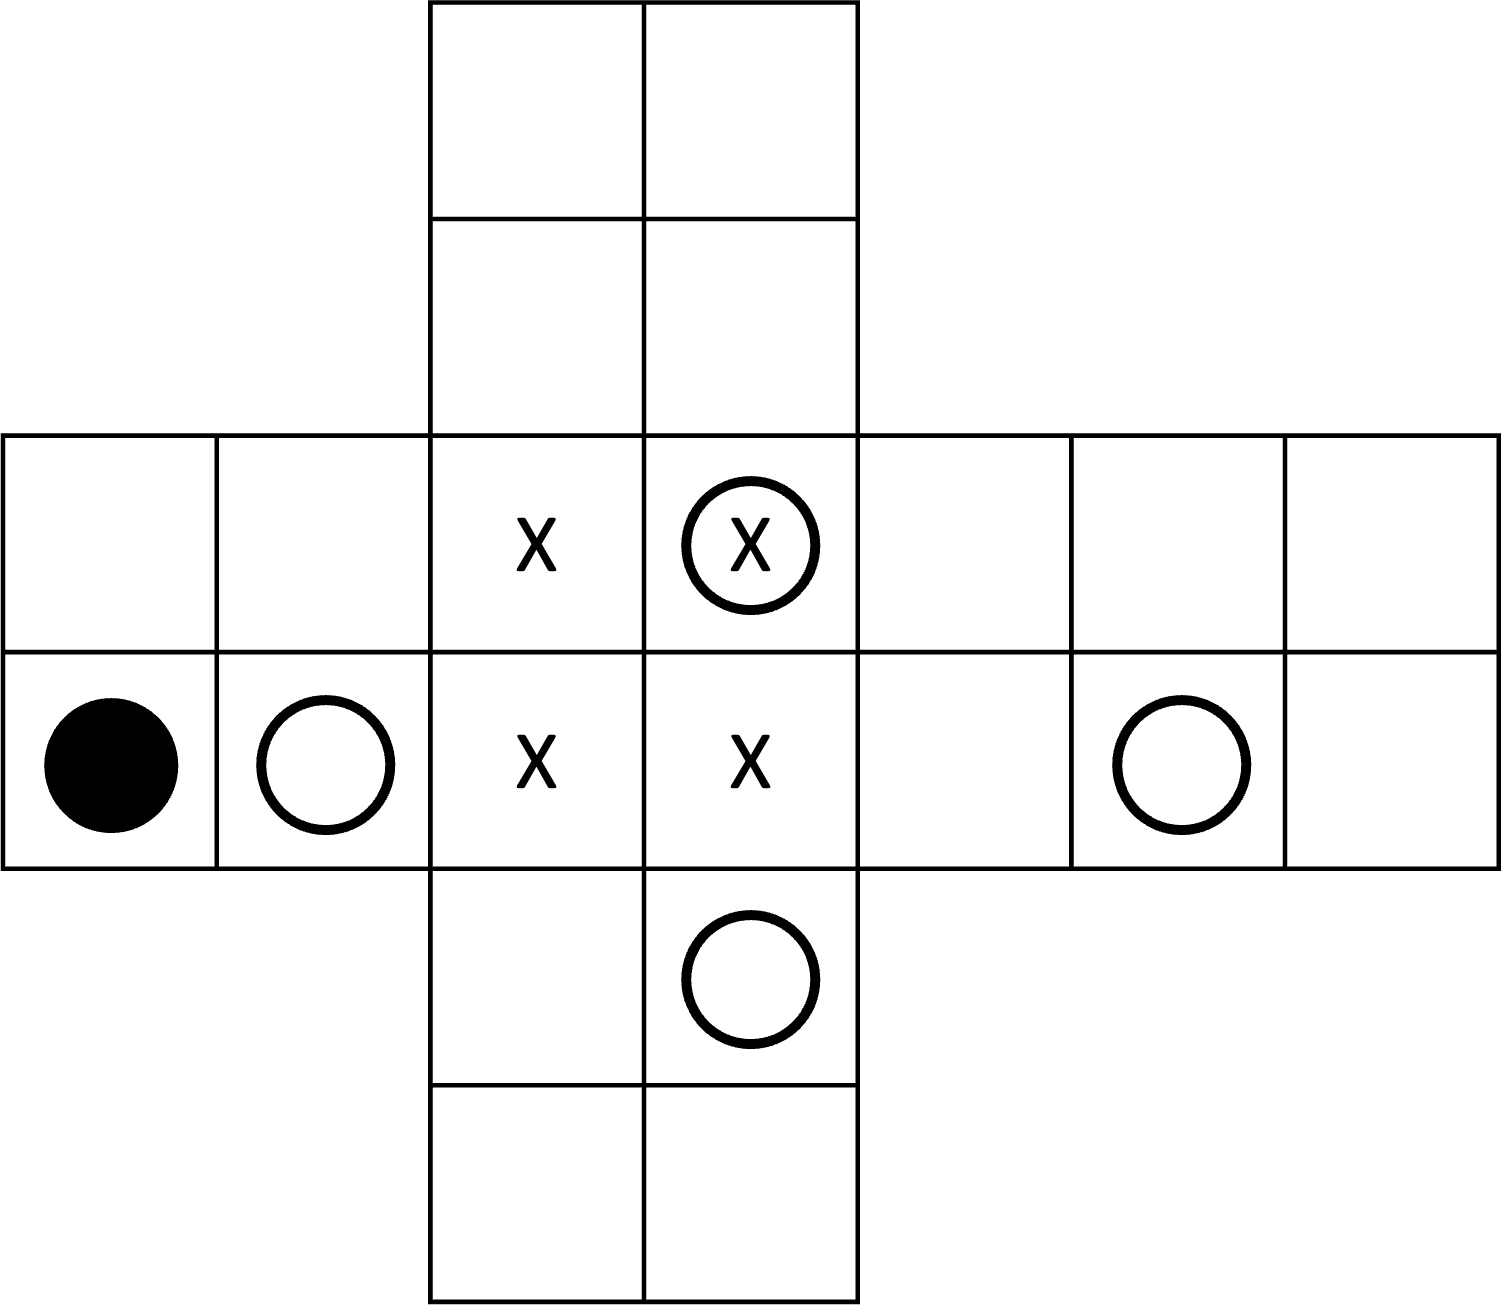
\includegraphics[scale=0.3]{../images/L1_ShuntingGame.png}
    \end{center}
\end{frame}

% Slide 53
\begin{frame}{Z Specification Case Study: Shunting Game (Writing the Specification)}
    \begin{columns}[t]
        \begin{column}{0.33\textwidth}
            \begin{scriptsize}
                \begin{schema}{Shunting}
                    bposn : Board\\
                    wposn : \power Board\\
                    score : \nat
                    \where
                    bposn \not \in wposn \wedge \#wposn = 4
                \end{schema}
            \end{scriptsize}
        \end{column}
        \begin{column}{0.33\textwidth}
            \begin{scriptsize}
            \begin{schema}{ShuntingInit}
                bposn = (1, 4)\\
                wposn = \set{(2, 4), (4, 3), (4, 5), (6, 4)}\\
                score = 0
            \end{schema}
            \end{scriptsize}
        \end{column}
        \begin{column}{0.33\textwidth}
            \begin{center}
                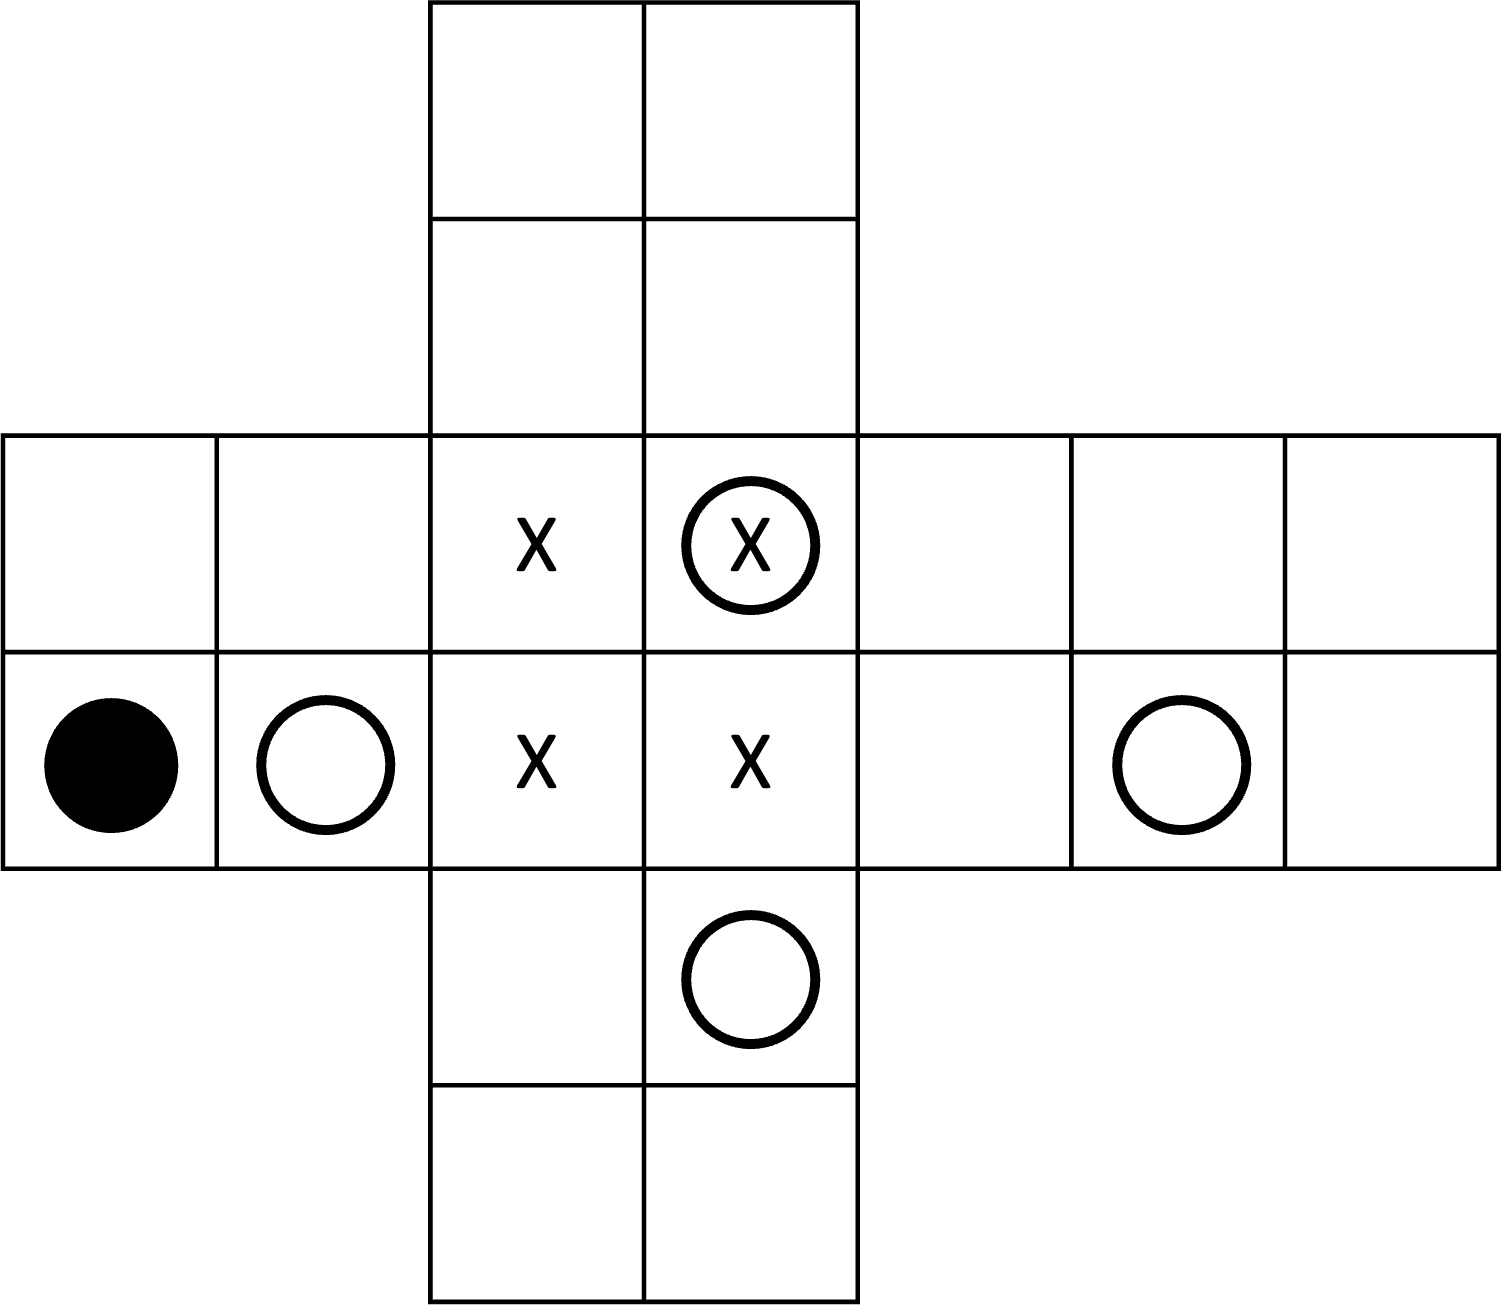
\includegraphics[scale=0.3]{../images/L1_ShuntingGame.png}
            \end{center}
        \end{column}
    \end{columns}
    \begin{columns}[t]
        \begin{column}{0.25\textwidth}
            \begin{scriptsize}
                \begin{schema}{Over}
                    \Xi Shunting \\
                    score! : \nat \\
                    \where
                    wposn = over \\
                    score! = score
                \end{schema}
            \end{scriptsize}
        \end{column}
        \begin{column}{0.75\textwidth}
            \begin{scriptsize}
            \begin{schema}{Move}
                \Delta Shunting
                \where
                wposn \neq over \\
                bposn' \underline{ next } bposn \\
                bposn' \not \in wposn \implies wposn' = wposn \\
                bposn' \in wposn \implies wposn' = (wposn - {bposn'}) \cup {beyond(bposn, bposn')} \\
                score' = score + 1
            \end{schema}
            \end{scriptsize}
        \end{column}
    \end{columns}
\end{frame}

% Slide 54
\begin{frame}{CSP Prelude: Automatic Reasoning \& Verification}
    \begin{itemize}
        \item Z Specification is good at \textbf{capturing high level requirements}.
        \item However, if we want to answer the following questions, we need a formal language that can perform automatic reasoning and verification.
        \begin{enumerate}
            \item What is a valid trace of moves in the Shunting Game?
            \item Is the goal state (a.k.a "over") reachable?
            \item If the goal state is reachable, are there any bad moves preventing the goal?
            \item What is the minimum number of moves to reach the goal?
        \end{enumerate}
        \item The answers to these questions would be answered in \textbf{process modelling using CSP} in the next section.
    \end{itemize}
    \begin{columns}
        \begin{column}{0.7\textwidth}
            \begin{center}
                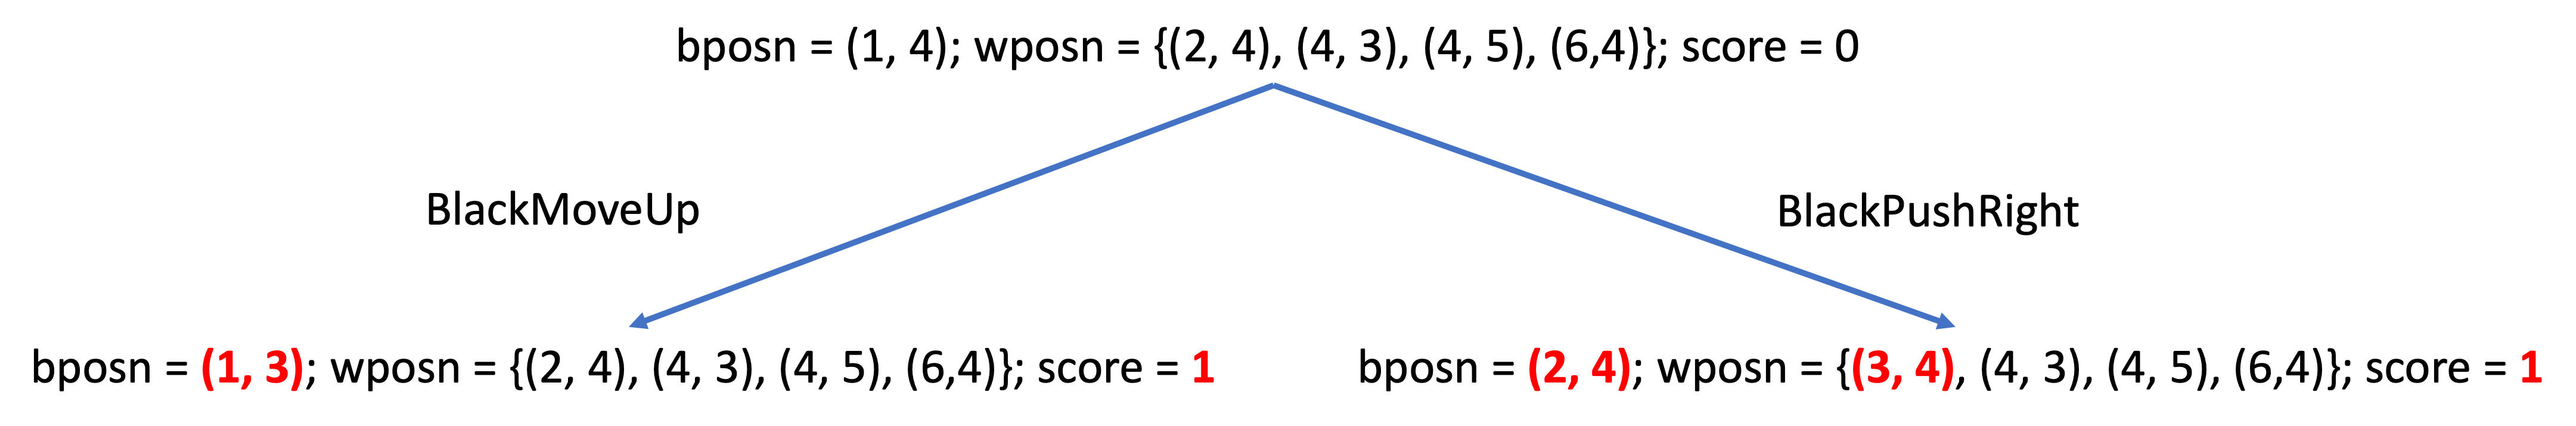
\includegraphics[scale=0.35]{../images/L1_ShuntingGameTree.png}
            \end{center}
        \end{column}
        \begin{column}{0.3\textwidth}
            \begin{center}
                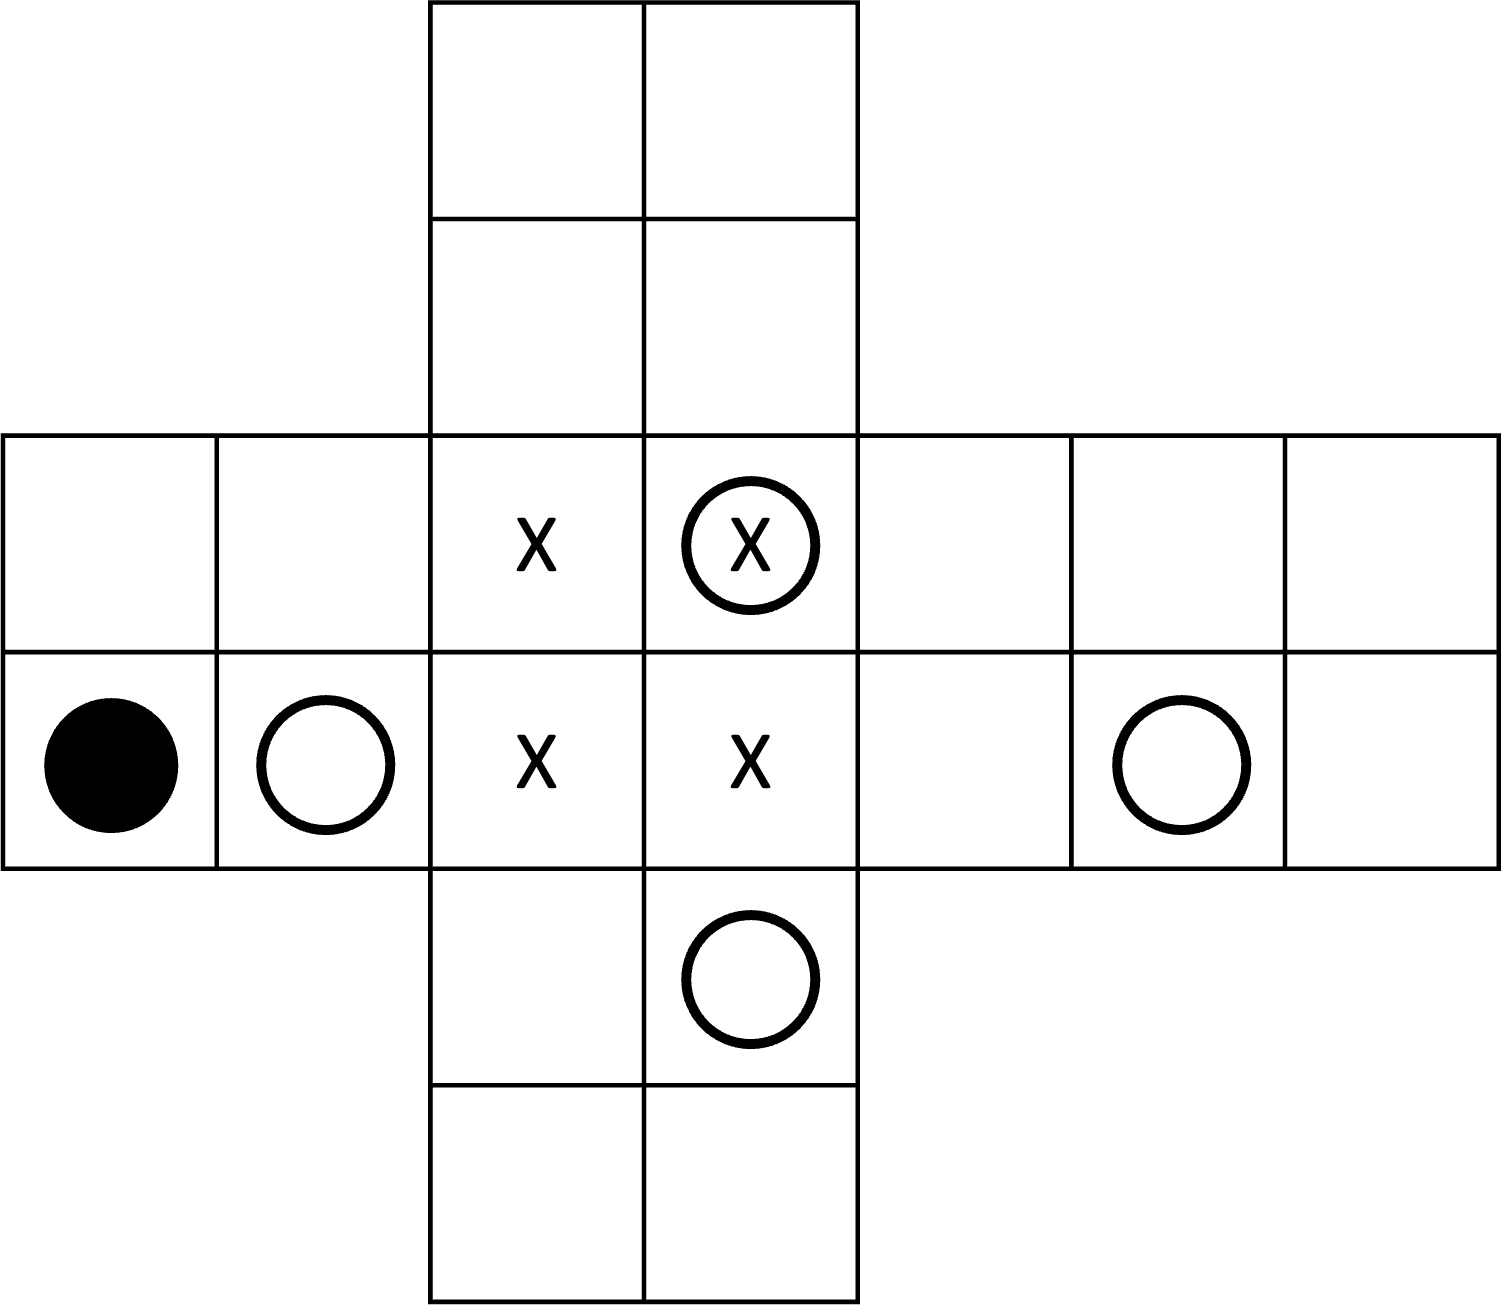
\includegraphics[scale=0.3]{../images/L1_ShuntingGame.png}
            \end{center}
        \end{column}
    \end{columns}
\end{frame}

% Slide 55
\section{Communicating Sequential Processes (CSP)}

% Slide 56
\begin{frame}{Introduction to CSP}
    \begin{itemize}
        \item \textbf{Communicating Sequential Processes (CSP)} is a formal language to describe patterns interaction between concurrent processes in computer systems.
        \item CSP was created by \textbf{Tony Hoare} to reason about the behaviour of concurrent systems.
        \item CSP provides \textbf{event based} notation primarily aimed at describing the sequencing of behaviour within a process and the synchronisation of behaviour (or communication) between processes.
        \item In CSP, there are two main fundamental concepts
        \begin{enumerate}
            \item Process
            \item Event
        \end{enumerate}
        \item Events represent a co-operative synchronisation between process and environment.
        \item Both process and environment may control the behaviour of each other by enabling or refusing certain events or sequences of events.
    \end{itemize}
\end{frame}

% Slide 57
\begin{frame}{Recap: Process State Model}
    \begin{itemize}
        \item To gain a better understanding of \textbf{Communicating Sequential Processes}, revisit the first half of \textbf{CS2106: Operating Systems} where Processes, Concurrency, Synchronisation and Semaphores were covered.
        \item The Process State Model is shown here to help you visualize potential process behaviour that can be modelled using CSP.
    \end{itemize}
    \begin{center}
        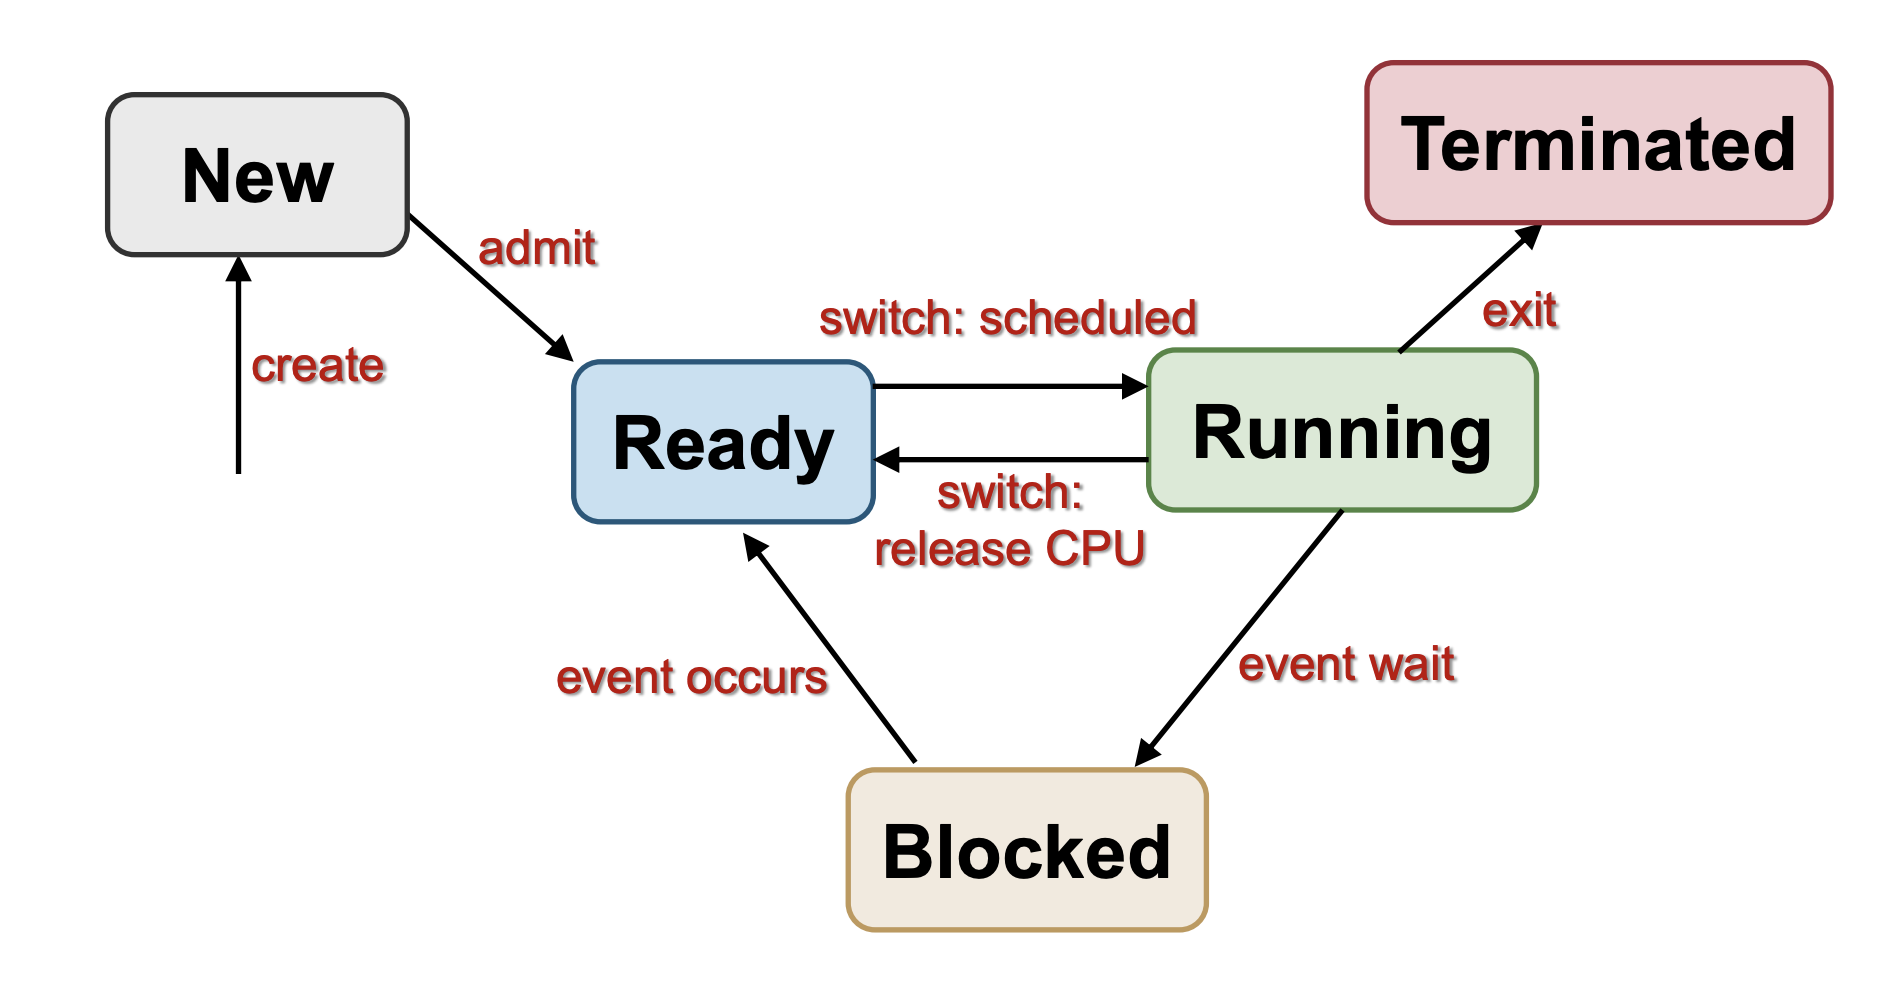
\includegraphics[scale=0.125]{../images/process.png}
    \end{center}
\end{frame}

% Slide 58
\begin{frame}{Specifying a Process}
    \begin{itemize}
        \item A process is determined or specified by what it can do.
        \item In other words, a process is defined by its behaviour, which are the events that we can observe.
        \item The perceived behaviour of a process will depend on the observer.
        \item In this course, we are mainly concerned with specifying the interaction between a system and its environment which is also the \textbf{external or visible behaviour}.
    \end{itemize}
\end{frame}

% Slide 59
\begin{frame}{Concepts in CSP: Events}
    \begin{itemize}
        \item A process engages in \textbf{events}.
        \item Each event is an atomic action.
        \begin{block}{Alphabet}
            The \textbf{set of events} a process can possibly engage in is the \textbf{alphabet} of the process.
        \end{block}
        \item Example: Chocolate Vending Machine
        \item Events for a chocolate vending machine
        \begin{enumerate}
            \item coin - insert a coin
            \item choc - extract a chocolate
        \end{enumerate}
        \item The alphabet of a chocolate vending machine is $\{coin, choc\}$
    \end{itemize}
\end{frame}

% Slide 60
\begin{frame}{Concepts in CSP: Trace}
    \begin{block}{Trace}
        A finite sequence of events
    \end{block}
    \begin{itemize}
        \item A deterministic process is specified by the set of processes denoting its possible behaviour.
        \item Any execution of the process will be one of these sequences.
        \item Example: The traces of the chocolate vending machine are:
        \begin{itemize}
            \item $\nil$
            \item $\trace{coin}$
            \item $\trace{coin, choc}$
            \item $\trace{coin, choc, coin}$
            \item $\ldots$
        \end{itemize}
        \item Any execution of the process will be one of the above sequences or traces. 
        \item If $s \cat t$ is a trace of a process, then $s$ is also a trace of a process. This means that set of traces is prefixed closed.
        \begin{itemize}
            \item Example: Let $s = \trace{coin, choc}, t = \trace{coin}$, then $s \cat t = \trace{coin, choc, coin}$.
        \end{itemize}
    \end{itemize}

\end{frame}

% Slide 61
\begin{frame}{Notations and Conventions}
    \begin{itemize}
        \item \textbf{Events} are denoted in \textbf{lower case}
        \begin{itemize}
            \item Example: $x, y, z$ are variables that denote events.
        \end{itemize}
        \item \textbf{Processes} are denoted in \textbf{upper case}
        \begin{itemize}
            \item Example: $X, Y, Z$ are variables that denote processes.
        \end{itemize}
        \item The \textbf{alphabet} of a process $P$ is denoted by $\alpha P$
        \item The set of traces of $P$ is denoted by \texttt{traces(P)}
        \item \textbf{Trace Notation}
        \begin{itemize}
            \item If $A$ is a set of events, then $\seq A$ denotes the set of all finite sequences of events from $A$.
            \item In this scenario, \texttt{$\alpha$ P = A} and \texttt{trace(P) = $\seq A$}
            \item Let $s, t : \seq A$, $s \cat t$ be the concatenation of $s$ with $t$.
            \item We define the relation $<=$ to be the \textbf{sequence prefix} of two sequences.
            \begin{axdef}
                <= : \seq A \rel \seq A
                \where
                s <= t \Leftrightarrow \exists u : \seq A \spot s \cat u = t
            \end{axdef}
            \item $s^n = s \cat s \cat s \cat \ldots \cat s$ denotes the event s concatenated with itself $n$ times.
        \end{itemize}
    \end{itemize}
\end{frame}

% Slide 62
\begin{frame}{Examples of Process Specification using CSP}
    \begin{enumerate}
        \item Let $STOP_{A}$ be the process with alphabet $A$ that can do nothing.
        \begin{itemize}
            \item $traces(STOP_{A}) = \{\nil\}$
        \end{itemize}
        \item Let CLOCK be the process with $\alpha CLOCK = {tick}$ which can 'tick' at any time.
        \begin{itemize}
            \item $traces(Clock) = tick^{*}$ where $* \geq 0$
        \end{itemize}
        \item Let VM be the process with $\alpha VM = \{coin, choc\}$ which repeatedly supplies a chocolate after a coin has been inserted.
        \begin{itemize}
            \item $traces(VM) = \{s: \seq \{coin, choc\} \mid \exists n : \nat \spot s <=$ $\trace{coin, choc}^{n} \}$
            \item Note: $<=$ is the sequence prefix relation from the previous slide.
        \end{itemize}
        \item Let WALK be a one-dimensional random walk process with $\alpha WALK = \{left, right\}$.
        \begin{itemize}
            \item $traces(WALK) = (left \vee right)^{*}$ where $* \geq 0$
        \end{itemize}
        \item Let LIFE be the process with $\alpha LIFE = \{beat\}$ which can stop (die) at any time.
        \begin{itemize}
            \item $traces(LIFE) = beat^{*}$ where $* \geq 0$
        \end{itemize}
    \end{enumerate}
\end{frame}

% Slide 63
\begin{frame}{CSP Syntax}
    \begin{enumerate}
        \item Prefix: $a \then P$
        \item Sequential Composition: $P;Q$
        \item Parallel Composition (Synchronous): $P \parallel[X] Q$
        \item Interleaving (Asynchronous): $P \interleave Q$
        \item Choice: $a \then P \extchoice b \then Q$
        \item Interrupt Process: $P$ $\nabla$ $e \then Q$
    \end{enumerate}

    \footnotetext{Note that in the \texttt{zed-csp} package, the interrupt symbol is $\interrupt$.}
\end{frame}

% Slide 64
\begin{frame}{Prefix}
    \begin{itemize}
        \item A process which may participate in \textbf{event a} then act according to \textbf{process description P} is written as: \texttt{a -> P}.
        \item \textbf{a} is the event prefix to \textbf{P}.
        \item The \textbf{event a} is initially enabled by the process and occurs as soon as it is requested by its environment. All other events are refused initially.
        \item The \textbf{event a} is sometimes referred to as the guard of the process.
        \item Examples
        \begin{enumerate}
            \item $VMU = coin \then STOP$
            \item $SHORTLIFE = (beat \then (beat \then STOP)) = beat \then beat \then STOP$
            \item $VMS = coin \then choc \then STOP$
        \end{enumerate}
    \end{itemize}
\end{frame}

% Slide 65
\begin{frame}{Sequential Composition ($P;Q$)}
    \begin{itemize}
        \item Let $\tick$ be the Termination event.
        \item The process which may only terminate is written as $SKIP$.
        \item Let $SKIP = \tick \then STOP$.
        \item The sequential composition of processes P and Q, written as $P;Q$, acts as P until P terminates by communicating $\tick$ and then proceeds to act as Q.
    \end{itemize}
\end{frame}

% Slide 66
\begin{frame}{Parallel Composition}
    \begin{itemize}
        \item The parallel composition of \textbf{processes P and Q} synchronised on the \textbf{event set X} is written as $P \parallel[X] Q$.
        \item No event from $X$ may occur in $P \parallel[X] Q$ unless \textbf{jointly enabled} by both P and Q.
        \item When events from $X$ occur, they occur in both P and Q simultaneously, and are referred to as \textbf{synchronisations}. 
        \item Events \textbf{not from X} may occur in either P or Q seperately \textbf{but not jointly}.
        \item Example: $(a \then P) \parallel[a] (c \then a \then Q)$
        \begin{itemize}
            \item All \textbf{a} events must be Synchronous between the two processes.
        \end{itemize}
        \item Often, it is simply written as $P \parallel Q$ where the common event set $X = \alpha P \cap \alpha Q$ is omitted.
        \begin{itemize}
            \item When $P \parallel Q$ is given, we still know that all common events in $X = \alpha P \cap \alpha Q$ must be synchronous between P and Q.
        \end{itemize}
    \end{itemize}
\end{frame}

% Slide 67
\begin{frame}{Interleaving}
    \begin{itemize}
        \item $P \interleave Q$ denotes an asynchronous parallel composition between two processes \textbf{P} and \textbf{Q}.
        \item Both components \textbf{P} and \textbf{Q} \textbf{execute concurrently} without any synchronisation.
        \item Example: $((a \then P) \interleave (c \then a \then Q))$
        \begin{itemize}
            \item One possible trace is $\trace{c, a, a}$, after which the process acts as $P \interleave Q$
            \begin{enumerate}
                \item $c$ from $c \then a \then Q$ is engaged, leaving us with $((a \then P) \interleave (a \then Q))$
                \item $a$ from $a \then P$ is engaged, leaving us with $(P \interleave (a \then Q))$
                \item $a$ from $a \then Q$ is engaged, leaving us with $P \interleave Q$
            \end{enumerate}
            \item Another possible trace is $\trace{a, c, a}$, after which the process acts as $P \interleave Q$
            \begin{enumerate}
                \item $a$ from $a \then P$ is engaged, leaving us with $(P \interleave (c \then a \then Q))$
                \item $c$ from $c \then a \then Q$ is engaged, leaving us with $(P \interleave (a \then Q))$
                \item $a$ from $a \then Q$ is engaged, leaving us with $P \interleave Q$
            \end{enumerate}
        \end{itemize}
    \end{itemize}
\end{frame}

% Slide 68
\begin{frame}{Choice}
    \begin{itemize}
        \item In a general choice, $(a \then P) \extchoice (b \then Q)$, the process begins with both events \textbf{a} and \textbf{b} enabled.
        \item The subsequent behaviour depends on the event which occured.
        \begin{itemize}
            \item If the event which occured is \textbf{a}, the process will act as \textbf{P} afterwards.
            \item If the event which occured is \textbf{b}, the process will act as \textbf{Q} afterwards.
        \end{itemize}
        \item There are other types of choices, namely external or internal choice in the CSP syntax.
        \item For most cases, general choice is sufficient, hence in this module, we focus on general choice only.
        \item Example: $(a \then P) \extchoice (c \then a \then Q)$
        \begin{itemize}
            \item If the first event is \textbf{a}, after which the process acts as $P$.
            \item If the first event is \textbf{c}, after which the process acts as $a \then Q$.
        \end{itemize}
    \end{itemize}
\end{frame}

% Slide 69
\begin{frame}[fragile]
    \frametitle{Interrupt}
    \begin{itemize}
        \item The interrupt process $P$ $\nabla$ $e \then Q$ behaves as \textbf{process P} until the first occurrence of \textbf{event e} which then the control passes to \textbf{process Q}. 
        \item When coding the specification, the keyword \textbf{interrupt} is used instead of the symbol $\nabla$. 
        \item For the System process, the first event can be a routine or an exception.
        \item After that, it still behaves as a System process.      
    \end{itemize}
    \footnotetext{Note that in the \texttt{zed-csp} package, the interrupt symbol is $\interrupt$.}
\begin{lstlisting}
Err() = exception -> Err();
Routine() = routine -> Routine();
ExceptionHandling() = Routine() interrupt exception -> ExceptionHandling();
System = Err() || ExceptionHandling();
\end{lstlisting}

\end{frame}

% Slide 70
\begin{frame}[fragile]
\frametitle{Concurrency Example \#1}
We are given the following system specification in CSP
\begin{lstlisting}
VMC = coin -> ((choc -> VMC)[](bisc -> VMC));
CHOCLOV = choc -> CHOCLOV [] coin -> choc -> CHOCLOV;
#alphabet VMC{coin, choc, bisc};
#alphabet VMC{coin, choc, bisc};
System = VMC || CHOCLOV;
\end{lstlisting}

\begin{itemize}
\item Semi-colon marks the end of each statement.
\item When coding process specifications in CSP, we use the keyword \textbf{\#alphabet}, instead of the symbol $\alpha$.
\item The only possible trace for this example is $\trace{coin, choc}^{n}$ for $n : \nat_1$ after which the system acts as $VMC \parallel CHOCLOV$.
\begin{itemize}
    \item As defined in lines 3 and 4 of the specification, the common events are the alphabets of VMC and CHOCLOV which are \textbf{coin}, \textbf{choc} and \textbf{bisc}.
    \item However, the process \textbf{CHOCLOV} does not have the event \textbf{bisc}.
    \item In VMC, the \textbf{coin} event has to be engaged first before we can engage $choc \then VMC$
    \item Hence, both VMC and CHOCLOV engages in the \textbf{coin} event first then the \textbf{choc} event before acting as $VMC \parallel CHOCLOV$ again.
\end{itemize}
\end{itemize}
\end{frame}

% Slide 71
\begin{frame}[fragile]
\frametitle{Concurrency Example \#2}
We are given the same specification as the previous slide in CSP except that we now do not define the alphabet for the \textbf{VMC} and \textbf{CHOCLOV} processes.
\begin{lstlisting}
VMC = coin -> ((choc -> VMC)[](bisc -> VMC));
CHOCLOV = choc -> CHOCLOV [] coin -> choc -> CHOCLOV;
System = VMC || CHOCLOV;
\end{lstlisting}
\begin{itemize}
\item If we did not explicity define the alphabet for each process, it can be \textbf{auto inferred}.
\begin{itemize}
    \item $\alpha VMC = \{coin, choc, bisc\}$
    \item $\alpha CHOCLOV = \{coin, choc\}$
\end{itemize}
\item In this specification the system may deadlock with the following trace $\trace{coin, bisc}$.
\begin{itemize}
    \item After $\trace{coin, bisc}$, no event is possible.
    \item This is because now the \textbf{bisc} event is not common to both \textbf{VMC} and \textbf{CHOCLOV} processes.
    \item Hence, the \textbf{bisc} event can occur seperately.
    \item After $\trace{coin, bisc}$ has occurred, the system would be stuck at $VMC \parallel choc \then CHOCLOV$.
    \item Since \textbf{coin} and \textbf{choc} are common events, neither events can be engaged synchronously as \textbf{coin} is a prefix for \textbf{choc}.
\end{itemize}
\end{itemize}
\end{frame}

% Slide 72
\begin{frame}[fragile]
\frametitle{Concurrency Example \#3}
We are given the following system specification in CSP
\begin{lstlisting}
VMH = on -> coin -> choc -> off -> VMH;
CUST = on -> ((coin -> bisc -> CUST) [] (curse -> coin -> choc -> CUST));
System = VMH || CUST;
\end{lstlisting}
\begin{itemize}
    \item The common events between \textbf{VMH} and \textbf{CUST} are \textbf{on}, \textbf{coin} and \textbf{choc} and they must occur synchronously in the two processes.
    \item $\trace{on, curse, coin, choc, off}$ is a possible trace.
    \begin{itemize}
        \item After the trace, the process will still behave as a System process.
    \end{itemize}
    \item Deadlocks can occur with the following trace $\trace{on, coin, bisc}$
    \begin{itemize}
        \item The system will be stuck at $choc \then off \then VMH \parallel CUST$ and no event can be engaged.
    \end{itemize}
\end{itemize}
\end{frame}

% Slide 73
\begin{frame}[fragile]
\frametitle{Concurrency Example \#4}
We are given the following system specification in CSP
\begin{lstlisting}
SLOWALK = left -> rest -> SLOWALK [] right -> rest -> SLOWALK;
SLOCLIMB = up -> rest -> SLOCLIMB [] down -> SLOCLIMB;
System = SLOWALK || SLOCLIMB;
\end{lstlisting}

Are the following traces possible?
\begin{enumerate}
    \item $\trace{up, rest}$
    \begin{itemize}
        \item No. The common event between \textbf{SLOWALK} and \textbf{SLOCLIMB} is \textbf{rest}.
        \item $\trace{up, left, rest}$ and $\trace{up, right, rest}$ are possible traces.
    \end{itemize}
    \item $\trace{\ldots, up, rest}$ where up may not the first event.
    \begin{itemize}
        \item Yes. For example $\trace{left, up, rest}$ and $\trace{right, up, rest}$.
    \end{itemize}
\end{enumerate}

\end{frame}

% Slide 74
\begin{frame}{Laws for Concurrency}
    \begin{itemize}
        \item Law 1: $P \parallel Q = Q \parallel P$
        \item Law 2: $P \parallel (Q \parallel R) = (P \parallel Q) \parallel R$
        \item Law 3: $P \parallel STOP_{\alpha P} = STOP_{\alpha P}$
    \end{itemize}
    Let...
    \begin{enumerate}
        \item $a \in (\alpha P - \alpha Q)$
        \item $b \in (\alpha Q - \alpha P)$
        \item $\{c, d\} \subseteq (\alpha P \cap \alpha Q)$
    \end{enumerate}
    \begin{itemize}
        \item Law 4A: $(c \then P) \parallel (c \then Q) = c \then (P \parallel Q)$
        \item Law 4B: $(c \then P) \parallel (d \then Q) = STOP$ if $c \neq d$
        \item Law 5A: $(a \then P) \parallel (c \then Q) = a \then (P \parallel (c \then Q))$
        \item Law 5A: $(c \then P) \parallel (b \then Q) = b \then ((c \then P) \parallel Q)$
        \item Law 6: $(a \then P) \parallel (b \then Q) = a \then (P \parallel (b \then Q)) \extchoice b \then((a \then P) \parallel Q)$
    \end{itemize}
\end{frame}

% Slide 75
\begin{frame}{Channel}
    \begin{itemize}
        \item Processes may communicate through channels.
        \item A channel is like a message buffer for one process to send a value to another process.
        \item A channel event is written as one of the following forms:
        
        \begin{tabular}{|l|l|}
            \hline
                \textbf{Form} & \textbf{Description} \\ 
            \hline
                $c!n$ & Channel Output. This event occurs when a process writes $n$ (a value) \\ & to the tail of channel c's buffer\\
            \hline
                $c?n$ & Channel Input. This event occurs when a process reads a value from \\ & the head of channel c's buffer to a local variable n\\
            \hline
                $c.n$ & Channel output and its matching channel input are engaged together\\ & by two processes.\\
            \hline
        \end{tabular}
    \end{itemize}
\end{frame}

% Slide 76
\begin{frame}[fragile]
    \frametitle{Channel Example}
    Suppose we are given the following specification in CSP.
\begin{lstlisting}[language=C]
channel c 1; // Channel with buffer size = 1
Sender(i) = c!i -> Sender(i);
Receiver() = c?x -> a.x -> Receiver();
System() = Sender(5) ||| Receiver();
\end{lstlisting}

\begin{itemize}
    \item Note: A process can have optional parameters, eg: Sender(i)
    \item The first event must be c!5 since c's buffer is empty.
    \item The second event must be c?5 since c's buffer size is 1.
    \item The third event can either be c!5 or a.5
\end{itemize}

\end{frame}

% Slide 77
\begin{frame}[fragile]
    \frametitle{Channel Example: Synchronous Buffer}
    Suppose we are given the following specification in CSP.
\begin{lstlisting}[language=C]
channel c 0; // Synchronous Buffer
Sender(i) = c!i -> Sender(i);
Receiver() = c?x -> a.x -> Receiver();
System() = Sender(5) ||| Receiver();
\end{lstlisting}

\begin{itemize}
    \item Note: A synchronous buffer is defined by setting the buffer size to 0.
    \item The first event must be c.5, since the sender must write to the c's buffer and the reciever must read from c's buffer simultaneously.
    \item The second event must be a.5
\end{itemize}

\end{frame}

% Slide 78
\begin{frame}[fragile]
\frametitle{CSP Model Checkers: Automatic Reasoning}
\begin{itemize}
    \item A CSP Model Checker can check if a property is always satisfied.
    \item In the next part, we will explore how we can verify certain properties of our process model using PAT (CSP\#).
    \item Suppose we are given the specification of the \textbf{Dining Philosophers Problem}.
\end{itemize}
\begin{lstlisting}[language=C]
#define N 2;
Phil(i) = get.i.(i+1)%N -> get.i.i -> eat.i -> put.i.(i+1)%N -> put.i.i -> Phil(i);
Fork(x) = get.x.x -> put.x.x -> Fork(x) [] get.(x-1)%N.x -> put.(x-1)%N.x -> Fork(x);
College() = ||x:{0..N-1}@(Phil(x)||Fork(x));
#assert College() deadlockfree; // Check if a property is satisifed.
\end{lstlisting}
\begin{itemize}
    \item $\parallel x : \{1 \upto n\} \at P(x)$ is equivalent to $P(1) \parallel \ldots \parallel P(n)$
    \item \texttt{\#assert College() deadlockfree} is the property we want to verify.
    \item If the property isn't always True, the Model Checker gives a counter example: $\trace{get.1.0, get.0.1}$
\end{itemize}
\end{frame}

% Slide 79
\section{Process Analysis Toolkit (PAT)}

% Slide 80
\begin{frame}{Introduction to Process Analysis Toolkit (PAT)}
\begin{itemize}
    \item The \hyperlink{https://www.comp.nus.edu.sg/~pat/OnlineHelp/index.htm}{Process Analysis Toolkit} is a self-contained framework to support composing, simulating and reasoning of concurrent, real-time systems and other possible domains.    
    \item In PAT 3.5, there are 11 developed modules provided to model a variety of different systems ranging from \textbf{Communicating Sequential Processes (CSP) Module}, \textbf{Real-Time System Module} to the \textbf{Web Service Module}. 
    \item In this module, we will be focusing on the \textbf{Communicating Sequential Programs (CSP\#) module}
\end{itemize}
\end{frame}

% Slide 81
\begin{frame}{Introduction to PAT's CSP\#}
    \begin{itemize}
        \item PAT's CSP\# module supports a rich modeling language named CSP\#(pronounced 'CSP sharp', short for Communicating Sequential Programs) \item CSP\# combines high-level modeling operators like (conditional or non-deterministic) choices, interrupt, (alphabetized) parallel composition, interleaving, hiding, asynchronous message passing channel, etc., with programmer-favored low-level constructs like variables, arrays, if-then-else, while, etc $\ldots$
        \item CSP\# offers great flexibility on how to model systems. For instance, communication among processes can be either based on shared memory (using global variables) or message passing (using asynchronous message passing or CSP-style multi-party barrier synchronization).
        \item The high-level operators are based on the classic process algebra Communicating Sequential Processes (CSP). 
        \item The design principle for CSP\# is to maximally keep the original CSP as a sub-language of CSP\#, whilst offering a connection to the data states and executable data operations.
    \end{itemize}
\end{frame}

% Slide 82
\begin{frame}{Operational Semantics}
    \begin{itemize}
        \item Earlier, we want a way to automatically reason if a model satisfies a certain property. 
        \item Hence, we will need to study \textbf{Operational Semantics} to understand how a process transitions from one state to another during the execution of CSP Specification.
        \item \textbf{Operational Semantics} tell us at given a system state, what are the possible actions the system can perform and what are the outcomes (next state)?
        \begin{itemize}
            \item Example: $P \xrightarrow{a} Q$
            \item The above is read as: If process P engages event a, it will become process Q.
            \item In most cases the states are the process and actions are the events.
            \item We will see in later examples what are states and actions.
        \end{itemize}
        \item Operational Semantics can be presented using a set of inference rules in the following form similar to the philosophy of logic.
        
        \begin{axdef}
            Premises
            \where
            Conclusion
        \end{axdef}
    \end{itemize}
\end{frame}

% Slide 83
\begin{frame}{Operational Semantics: Primitives}
    \begin{itemize}
        \item STOP (A process that does nothing)
        \item SKIP
        \begin{axdef}
            \where
            SKIP \xrightarrow{\tick} STOP
        \end{axdef}
        SKIP can only engage the \textbf{termination event}, afterwards it becomes STOP.
        \item Prefixing
        \begin{axdef}
            \where
            (a \then P) \xrightarrow{a} P
        \end{axdef}
        $a \then P$ can only engage event \textbf{a}, afterwards it becomes process \textbf{P}.
    \end{itemize}
\end{frame}

% Slide 84
\begin{frame}{Operational Semantics}
\begin{columns}
    \begin{column}{0.25\textwidth}
    \textbf{General Choice}
    \begin{itemize}
        \item If P is choosen
    \end{itemize}
    \begin{axdef}
        P \xrightarrow{a} P'
        \where
        (P \extchoice Q) \xrightarrow{a} P'
    \end{axdef}
    \begin{itemize}
        \item If Q is chosen
    \end{itemize}
    \begin{axdef}
        Q \xrightarrow{a} Q'
        \where
        (P \extchoice Q) \xrightarrow{a} Q'
    \end{axdef}
    \end{column}
    \begin{column}{0.4\textwidth}
        \textbf{Sequential Composition}
        \begin{itemize}
            \item In process P;Q, P takes control first and Q starts only when P has finished.
            \item Let $\tick$ be the termination event.
        \end{itemize}
        \begin{axdef}
            P \xrightarrow{a} P'
            \where
            (P ; Q) \xrightarrow{a} (P' ; Q)
        \end{axdef}
        
        \begin{axdef}
            P \xrightarrow{\tick} P'
            \where
            (P \extchoice Q) \xrightarrow{\tick} Q
        \end{axdef}
    \end{column}
    \begin{column}{0.35\textwidth}
        \textbf{Interrupt}
        \begin{itemize}
            \item In process P $\nabla$ Q, whenever an event is engaged by Q, P is interrupted and the control is transferred to Q.
        \end{itemize}
        \begin{axdef}
            P \xrightarrow{a} P'
            \where
            (P \nabla Q) \xrightarrow{a} (P' \nabla Q)
        \end{axdef}

        \begin{axdef}
            Q \xrightarrow{a} Q'
            \where
            (P \nabla Q) \xrightarrow{a} Q
        \end{axdef}
    \end{column}
\end{columns}

\end{frame}

% Slide 85
\begin{frame}{Operational Semantics: Example \#1}
    \begin{itemize}
        \item Let $VMS = coin \then (choc \then VMS \extchoice bisc \then VMS)$ 
    \end{itemize}

    \begin{block}{Operation Semantics}
        Step 1. $VMS \xrightarrow{coin} (choc \then VMS \extchoice bisc \then VMS)$\\
        Step 2. $(choc \then VMS \extchoice bisc \then VMS) \xrightarrow{choc} VMS$\\
        Step 2. $(choc \then VMS \extchoice bisc \then VMS) \xrightarrow{bisc} VMS$
    \end{block}
    
\end{frame}

% Slide 86
\begin{frame}{Labelled Transition System (LTS)}
    \begin{itemize}
        \item A \textbf{Labelled Transition System} contains a set of states, an initial state (where the system starts from) and a labelled transition relation.
    \end{itemize}
    \begin{center}
        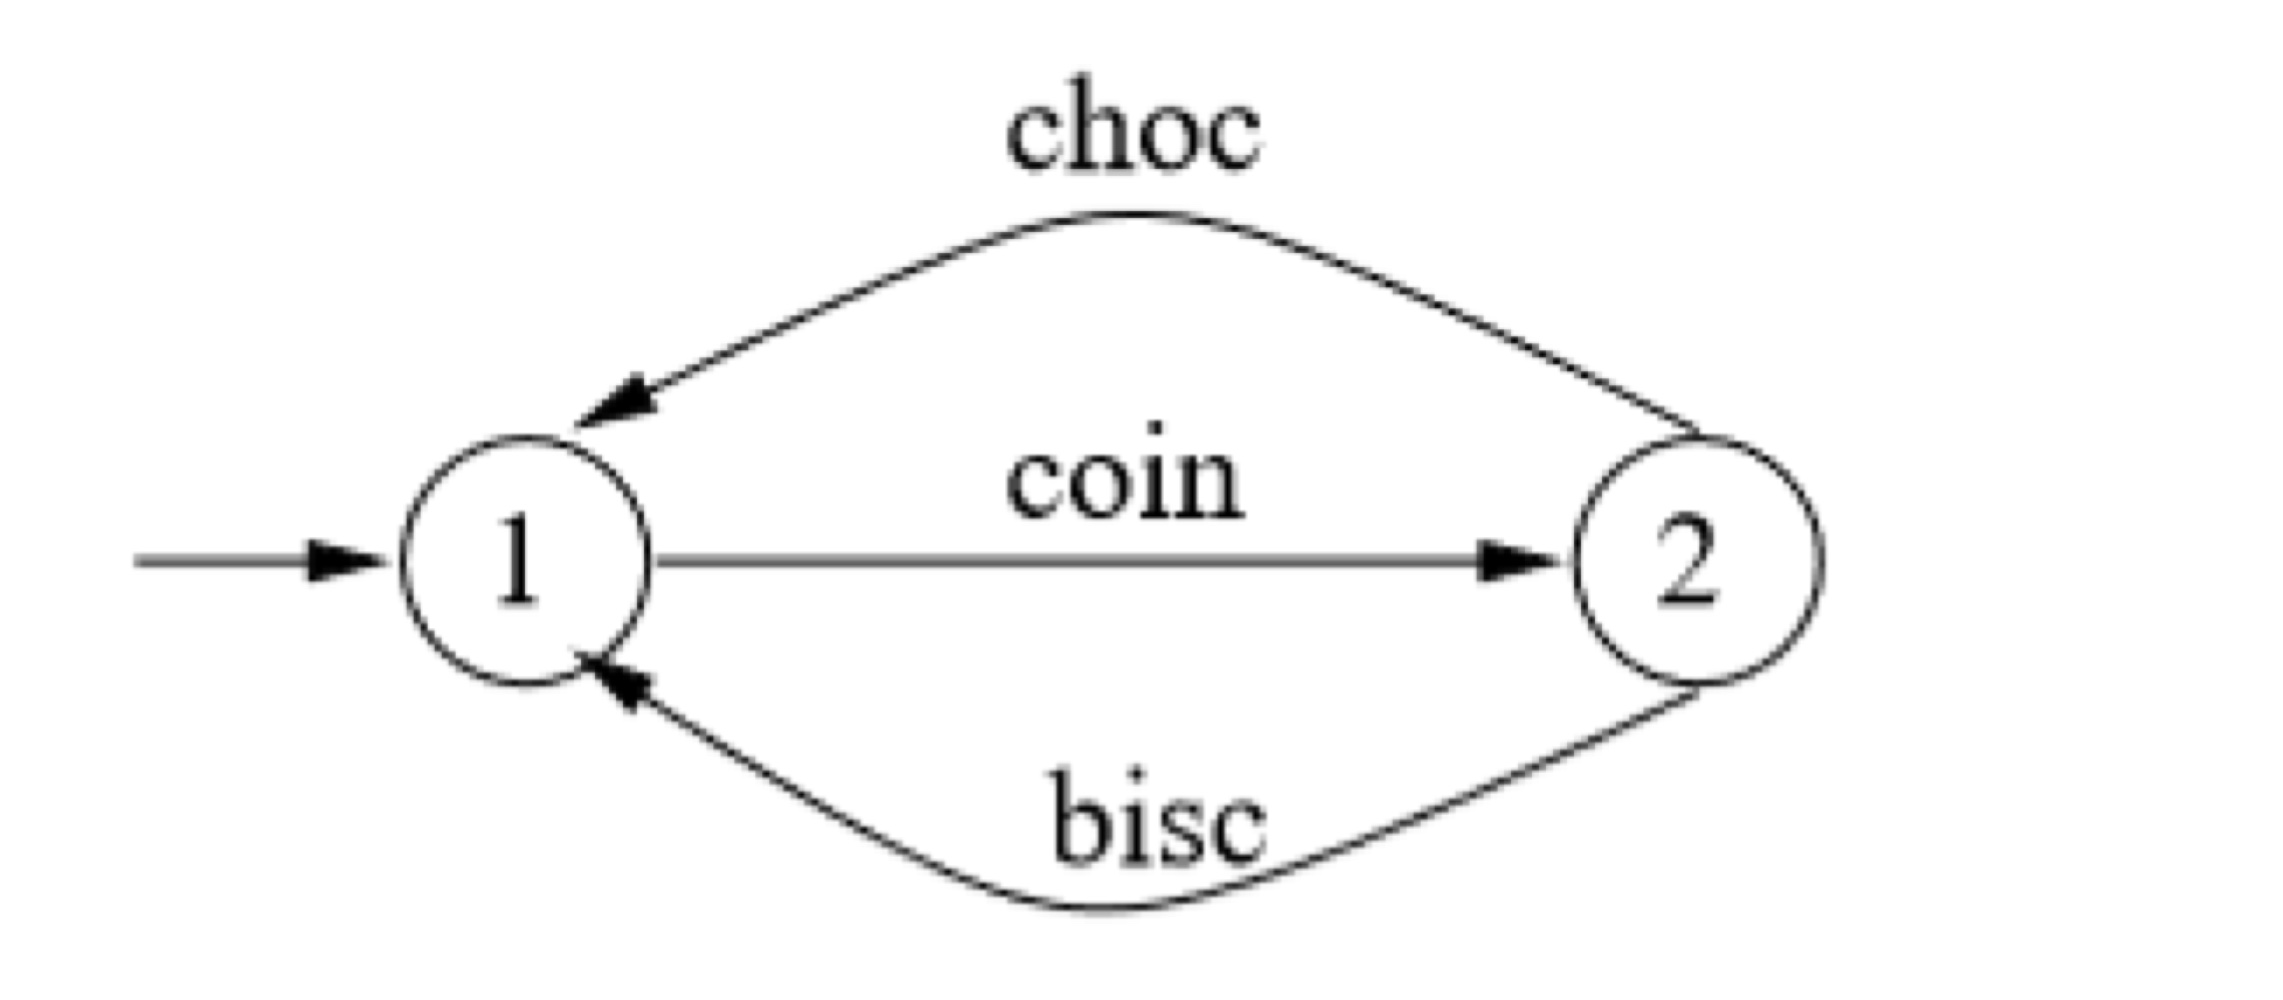
\includegraphics[scale=0.08]{../images/LTS.jpeg}
    \end{center}
    \begin{itemize}
        \item Let $VMS = coin \then (choc \then VMS \extchoice bisc \then VMS)$ 
        \item State 1 represents the process VMS.
        \item State 2 represents the process $(choc \then VMS \extchoice bisc \then VMS)$
    \end{itemize}
    \footnotetext[1]{The Labelled Transition System is a directed graph}
\end{frame}

% Slide 87
\begin{frame}{Operational Semantics}
    \begin{columns}
        \begin{column}{0.5\textwidth}
            \textbf{Interleaving}
            \begin{itemize}
                \item In process $P \interleave Q$, P and Q behaves independently.
                \item The exception is the termination, hence assume a is not $\tick$.
            \end{itemize}
            \begin{axdef}
                P \xrightarrow{a} P'
                \where
                (P \interleave Q) \xrightarrow{a} (P' \interleave Q)
            \end{axdef}
            \begin{axdef}
                Q \xrightarrow{a} Q'
                \where
                (P \interleave Q) \xrightarrow{a} (P \interleave Q')
            \end{axdef}
        \end{column}
        \begin{column}{0.5\textwidth}
            \textbf{Synchronization}
            \begin{itemize}
                \item In process $P \parallel[X] Q$, no event from X may occur unless jointly by both P and Q.
                \item When events from X do occur, they occur in P and Q simultaneously.
            \end{itemize}
            \begin{footnotesize}
                \begin{axdef}
                    P \xrightarrow{a} P' , a \not \in X
                    \where
                    (P \parallel[X] Q) \xrightarrow{a} (P' \parallel[X] Q)
                \end{axdef}
                \begin{axdef}
                    Q \xrightarrow{a} Q' , a \not \in X
                    \where
                    (P \parallel[X] Q) \xrightarrow{a} (P \parallel[X] Q')
                \end{axdef}
                \begin{axdef}
                    P \xrightarrow{a} P', Q \xrightarrow{a} Q' , a \in X
                    \where
                    (P \parallel[X] Q) \xrightarrow{a}  (P' \parallel[X] Q')
            \end{axdef}
            \end{footnotesize}
        \end{column}
    \end{columns}
\end{frame}

% Slide 88
\begin{frame}{Operational Semantics: Example \#2}
Given the process $a \then P \parallel[a] (c \then a \then Q)$
\begin{enumerate}
    \item $(a \then P \parallel[a] (c \then a \then Q)) \xrightarrow{c} (a \then P \parallel[a] (a \then Q))$
    
    Only event \textbf{c} can be engaged at first as \textbf{a} is a common event in both $a \then P$ and $c \then a \then Q$.

    \item $(a \then P \parallel[a] (a \then Q)) \xrightarrow{a} (P \parallel[a] Q)$
    
    Engage the common event \textbf{a} on both $a \then P$ and $a \then Q$.
\end{enumerate}
    
\end{frame}

% Slide 89
\begin{frame}{Operational Semantics: Example \#3}
    \begin{itemize}
        \item $VMC = coin \then (choc \then VMC \extchoice bisc \then VMC)$
        \item $CHOCLOV = choc \then CHOCLOV \extchoice coin \then choc \then CHOCLOV$
    \end{itemize}
    \begin{enumerate}
        \item How would the process $VMC \parallel[A] CHOCLOV$ behave when $A = \set{coin, choc, bisc}$
        \begin{itemize}
            \item Step 1: $VMC \parallel[A] CHOCLOV \xrightarrow{coin} (choc \then VMC \extchoice bisc \then VMC) \parallel[A] (choc \then CHOCLOV)$
            \item Step 2: $(choc \then VMC \extchoice bisc \then VMC) \parallel[A] (choc \then CHOCLOV) \xrightarrow{choc} VMC \parallel[A] CHOCLOV$
        \end{itemize}
    \end{enumerate}
    \begin{center}
        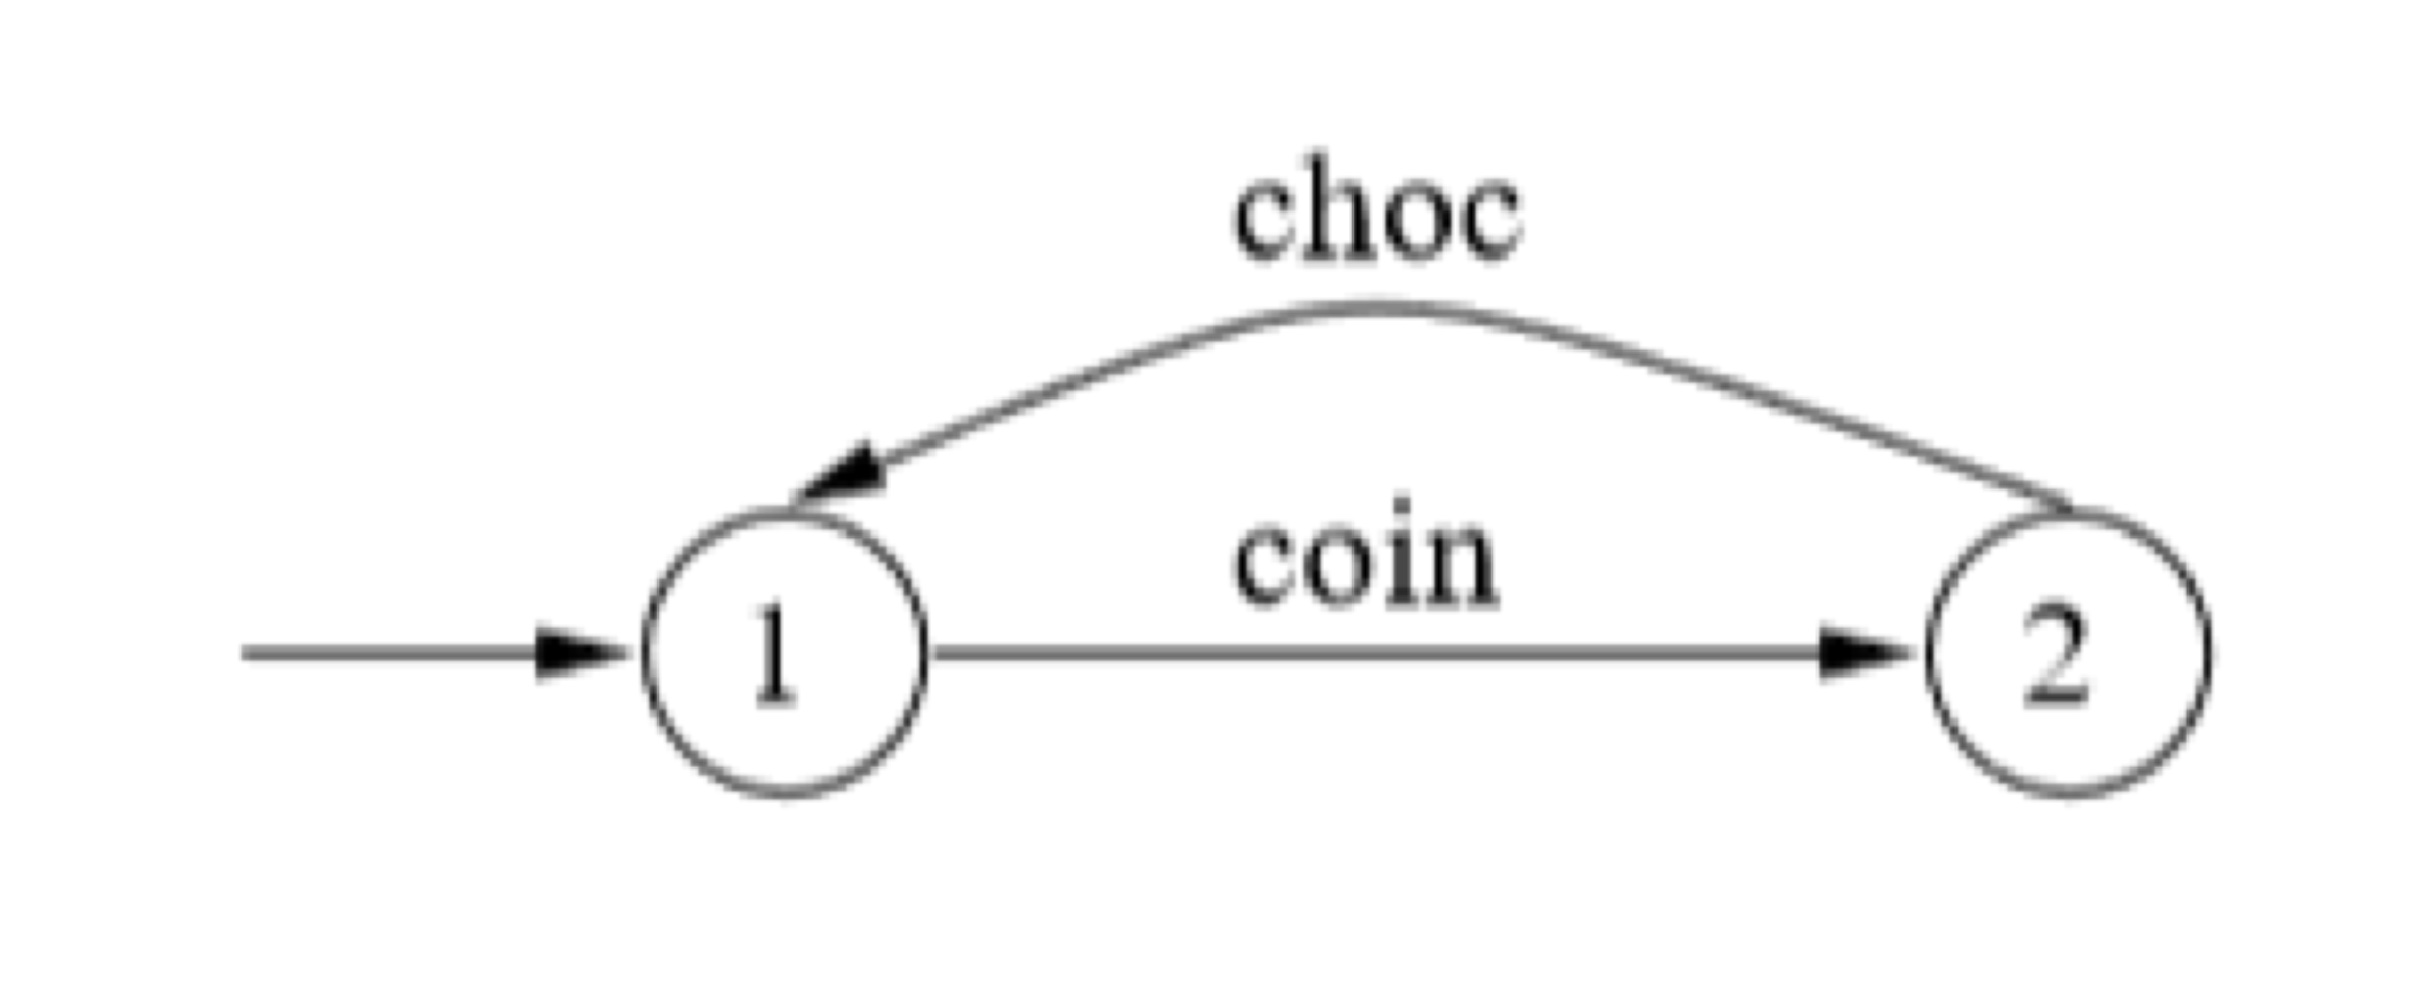
\includegraphics[scale=0.08]{../images/L3E3.jpeg}
    \end{center}
\end{frame}

% Slide 90
\begin{frame}{Operational Semantics Example: \#4}
    \begin{itemize}
        \item $VMC = coin \then (choc \then VMC \extchoice bisc \then VMC)$
        \item $CHOCLOV = choc \then CHOCLOV \extchoice coin \then choc \then CHOCLOV$
    \end{itemize}
    \begin{enumerate}
    \setcounter{enumi}{1}
    \item How would the process $VMC \parallel[\set{coin, choc}] CHOCLOV$ or equivalently $VMC \parallel CHOCLOV$ behave?
    \begin{itemize}
        \item Step 1: $VMC \parallel CHOCLOV \xrightarrow{coin} (choc \then VMC \extchoice bisc \then VMC) \parallel (choc \then CHOCLOV)$
        \item Step 2: $(choc \then VMC \extchoice bisc \then VMC) \parallel[A] (choc \then CHOCLOV) \xrightarrow{choc} VMC \parallel[A] CHOCLOV$
        \item Step 2: $(choc \then VMC \extchoice bisc \then VMC) \parallel[A] (choc \then CHOCLOV) \xrightarrow{choc} VMC \parallel[A] (choc \then CHOCLOV)$
    \end{itemize}
    \end{enumerate}
    \begin{center}
        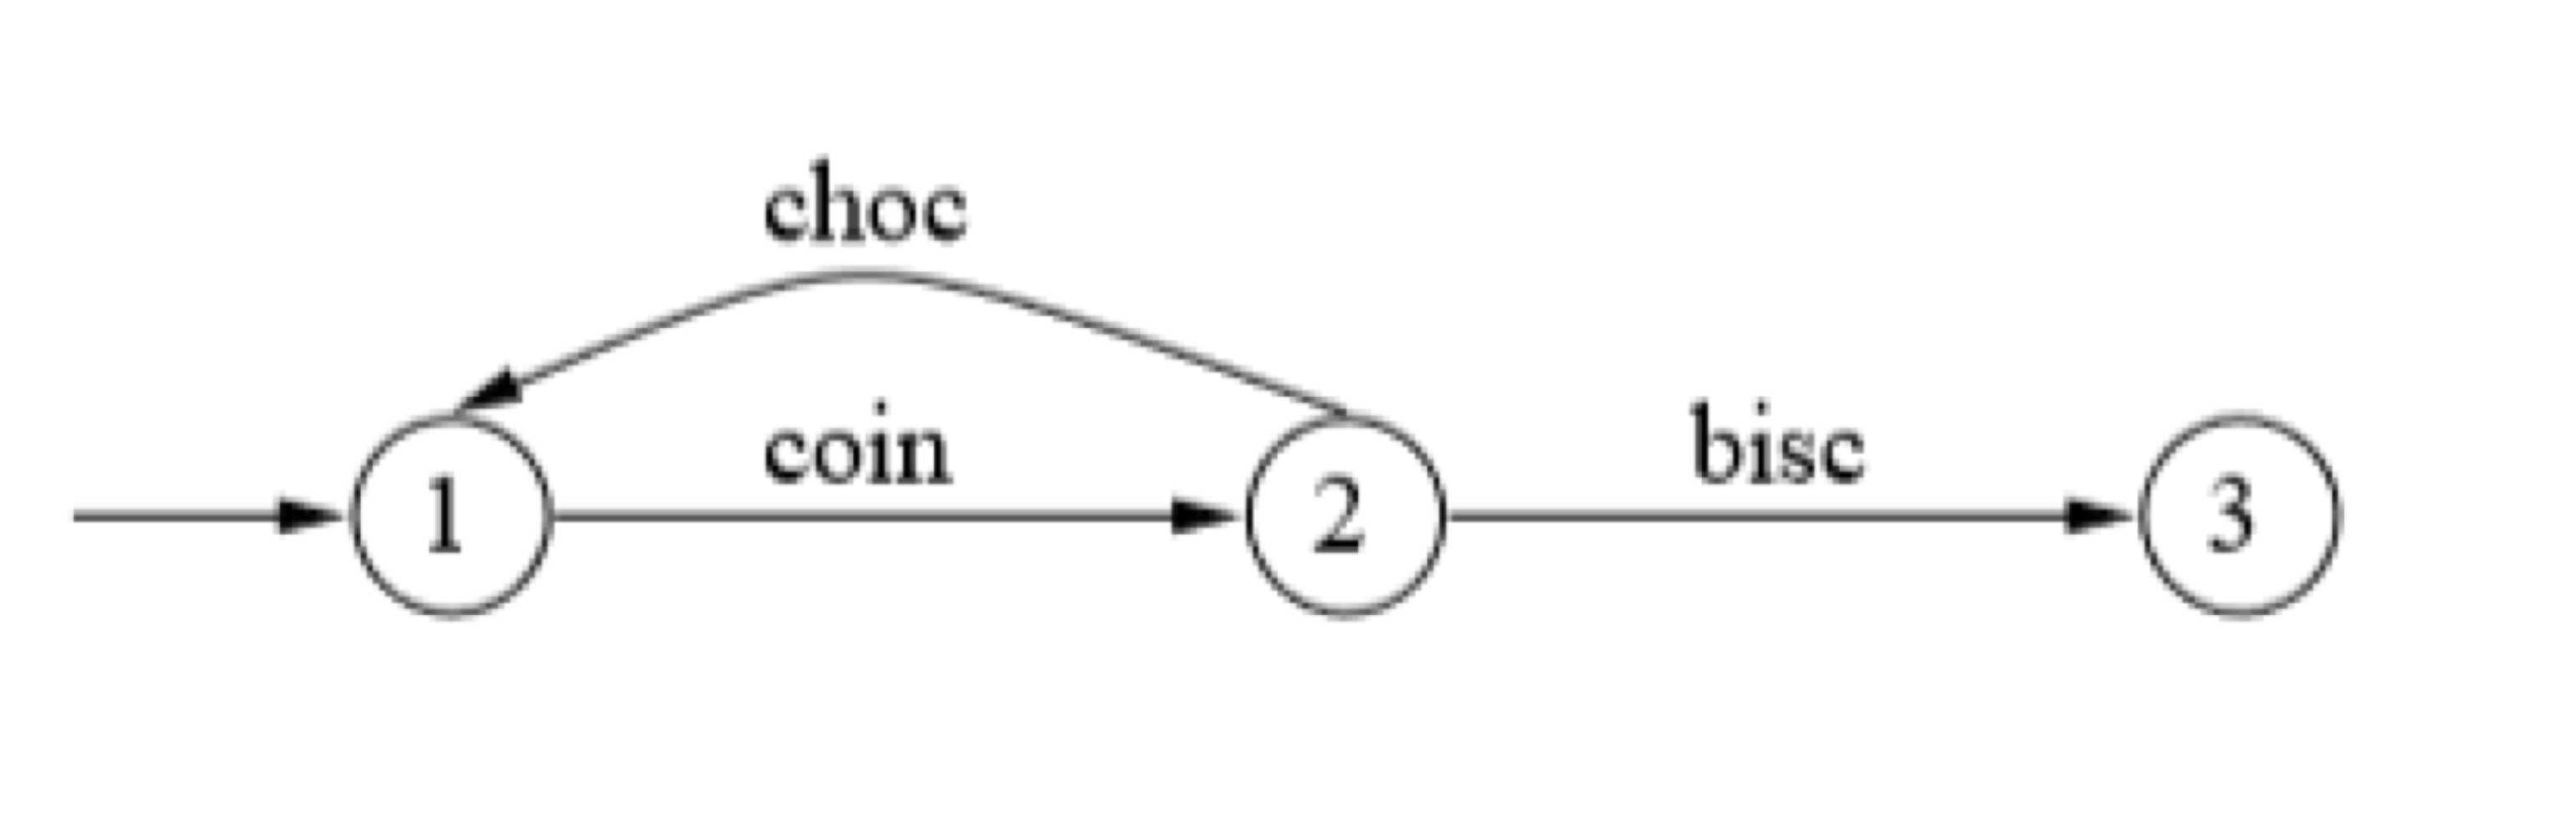
\includegraphics[scale=0.08]{../images/L3E4.jpeg}
    \end{center}
\end{frame}

% Slide 91
\begin{frame}[fragile]
    \frametitle{Case Study: Dining Philosophers}
    \begin{enumerate}
        \item Specify the dining philosophers 
\begin{lstlisting}
Alice = Alice.get.fork1 -> Alice.get.fork2 -> Alice.eat -> Alice.put.fork1 -> Alice.put.fork2 -> Alice
Bob = Bob.get.fork1 -> Bob.get.fork2 -> Bob.eat -> Bob.put.fork1 -> Bob.put.fork2 -> Bob
Fork1 = (Alice.get.fork1 -> Alice.put.fork1 -> Fork1) [] (Bob.get.fork1 -> Bob.put.fork1 -> Fork1)
Fork2 = (Alice.get.fork2 -> Alice.put.fork2 -> Fork2) [] (Bob.get.fork2 -> Bob.put.fork2 -> Fork2)
College = Alice || Bob || Fork1 || Fork2
\end{lstlisting}
        \item Get the alphabets of each process
        \begin{itemize}
            \item $\alpha Alice = \set{Alice.get.fork1, Alice.get.fork2, Alice.eat, Alice.put.fork1, Alice.put.fork2}$
            \item $\alpha Bob = \set{Bob.get.fork1, Bob.get.fork2, Bob.eat, Bob.put.fork1, Bob.put.fork2}$
            \item $\alpha Fork1 = \set{Alice.get.fork1, Alice.put.fork1, Bob.get.fork1, Bob.put.fork1}$
            \item $\alpha Fork2 = \set{Alice.get.fork2, Alice.put.fork2, Bob.get.fork2, Bob.put.fork2}$
        \end{itemize}
    \end{enumerate}
\end{frame}

% Slide 92
\begin{frame}{Case Study: Dining Philosophers}
\begin{enumerate}
    \setcounter{enumi}{2}
    \item Apply the operational semantics rule (one at a time) to build the Labelled Transition System.
    \begin{itemize}
        \item Alice can perform Alice.get.fork1
        \item Bob can perform Bob.get.Fork2
        \item Fork1 can perform Alice.get.fork1 or Bob.get.fork1
        \item Fork2 can perform Alice.get.fork2 or Bob.get.Fork2
        \item By rule syn3, College can perform either Alice.get.fork1 or Bob.get.fork2, and then a state of the form.
        \begin{center}
            $\cdots \parallel \cdots \parallel \cdots \parallel \cdots$
        \end{center}
    \end{itemize}
\end{enumerate}
\begin{center}
    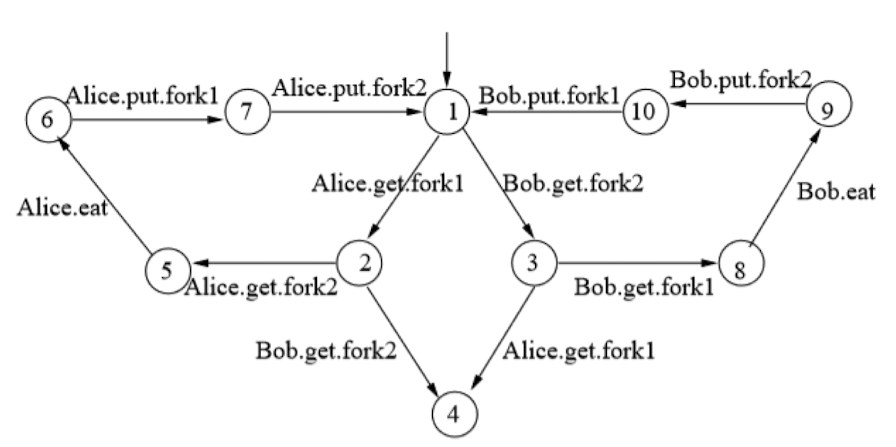
\includegraphics[scale=0.18]{../images/DiningPhilosophers.png}   
\end{center}
\end{frame}

% Slide 93
\begin{frame}{Case Study: Dining Philosophers}
    \begin{enumerate}
        \setcounter{enumi}{3}
        \item Analyze the Labelled Transition system
        \begin{itemize}
            \item Is the system deadlock-free?
            \item Will Alice or Bob starve to death?
        \end{itemize}
        \begin{center}
            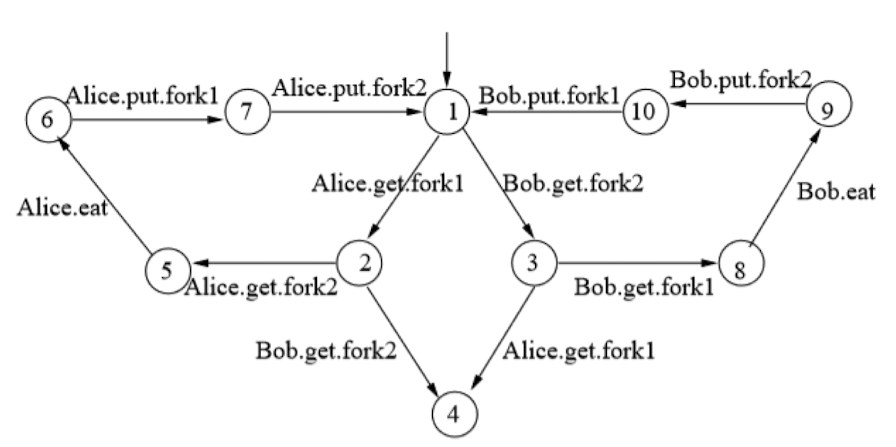
\includegraphics[scale=0.2]{../images/DiningPhilosophers.png}   
        \end{center}
    \end{enumerate}
\end{frame}

% Slide 94
\begin{frame}[fragile]
\frametitle{Safety}
\begin{itemize}
\item Safety means \textbf{something bad never happens}.
\item Examples
\begin{enumerate}
\item deadlock-freeness
\begin{lstlisting}
#assert College() deadlockfree;
\end{lstlisting}
The system never deadlocks
\item invariant
\begin{lstlisting}
#assert Bank() |= [] Value >= Debit;
\end{lstlisting}
The savings of a bank account must always be non-negative.
\end{enumerate}
\end{itemize}
\footnotetext[1]{'[]' signifies 'always' in Linear Temporal Logic.}
\footnotetext[2]{'$\mid =$' represents 'satisfisfaction' in Linear Temporal Logic.}
\end{frame}

% Slide 95
\begin{frame}{Verifying Safety}
    \begin{itemize}
        \item To verify safety, perform \textbf{reachability analysis} on the \textbf{Labelled Transition System}.
        \item A counterexample to the safety property is a finite execution which leads to a bad state.
        \item Perform either \textbf{Depth First Search (DFS)} or \textbf{Breadth First Search (BFS)} to search all reachable states for a 'bad' one.
        \item Example:
        \begin{center}
            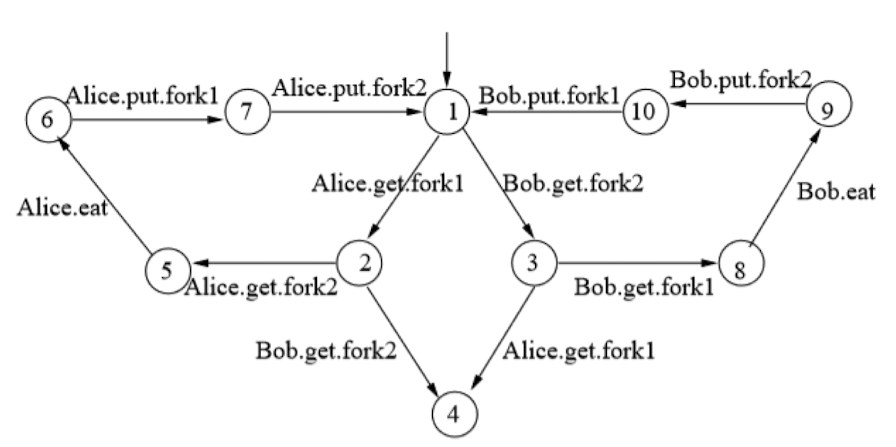
\includegraphics[scale=0.18]{../images/DiningPhilosophers.png}
        \end{center}
        \begin{enumerate}
            \item Depth First Search: $1 \then 2 \then 5 \then 7 \then 1 \then$ backtrack $\then 4 \then$ FOUND! 
            \item Breadth First Search: $1 \then 2 \then 3 \then 5 \then 4 \then$ FOUND!
        \end{enumerate}
    \end{itemize}
    \footnotetext[1]{State 4 is the bad state as there is no outgoing edges.}
\end{frame}

% Slide 96
\begin{frame}{Applications of Safety Verification}
Many properties can be formulated as a safety property and solved using \textbf{reachability analysis}.
\begin{enumerate}
    \item Mutual Exclusion: []!(more than one process accessing the critical section)
    \begin{itemize}
        \item There will never be more than one process accessing the critical section.
    \end{itemize}
    \item Security: [](only the authorized user can access the information)
    \begin{itemize}
        \item It is always the case that only the authorized user can access the information.
    \end{itemize}
    \item Program Analysis
    \begin{itemize}
        \item Arrays are always bounded.
        \item Pointers are always non-null
        \item etc...
    \end{itemize}
\end{enumerate}
\end{frame}

% Slide 97
\begin{frame}{Liveness}
    \begin{itemize}
        \item Liveness means \textbf{something good eventually happens}.
        \item Examples
        \begin{enumerate}
            \item A program is eventually terminating.
            \item A file writer is eventually closed.
            \item Both Alice and Bob eventually get to eat.
        \end{enumerate}
    \end{itemize}
\end{frame}

% Slide 98
\begin{frame}[fragile]
    \frametitle{Verifying Liveness}
    \begin{itemize}
        \item To verify liveness, perform \textbf{loop searching} on the \textbf{Labelled Transition System}.
        \item A counterexample to a liveness property is an infinite system execution during which the 'good' thing never happens.
        \begin{itemize}
            \item Example: An infinite loop fails the property that the program is eventually terminating.
        \end{itemize}
        \item We can search through the Labelled Transition System for a bad loop using \textbf{Nested Depth First Search} or \textbf{Strongly Connected Component based Search}
        \item Example
        \begin{columns}
            \begin{column}{0.45\textwidth}
                \begin{center}
                    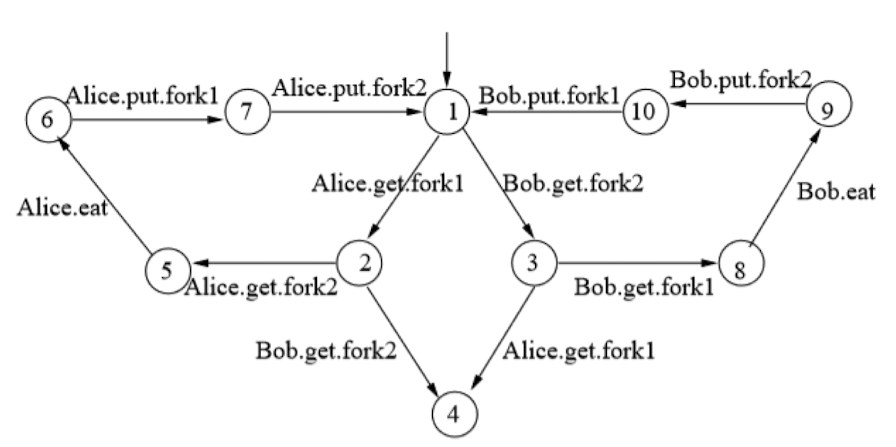
\includegraphics[scale=0.18]{../images/DiningPhilosophers.png}
                \end{center}
            \end{column}
            \begin{column}{0.55\textwidth}
                Assertion: Alice will always eventually eat. (\textbf{False})
\begin{lstlisting}
#assert College() |= Alice.eat
\end{lstlisting}
                \textbf{Counterexamples}
                \begin{itemize}
                    \item $\trace{Alice.get.fork1, Bob.get.fork2}$
                    \item $<Bob.get.fork2 \then Bob.get.fork1 \then Bob.eat \then$ \\ $Bob.put.fork2, \then Bob.put.fork1>^{*}$
                \end{itemize}
            \end{column}
        \end{columns}
   \end{itemize} 
\end{frame}

% Slide 99
\begin{frame}{CSP\#: Extending CSP}
    \begin{itemize}
        \item The original CSP has no shared variables, arrays, etc\dots
        \item PAT (CSP\#) extends it with data operations.
        \item Hence, the operational semantics must be updated to support data operations.
    \end{itemize}
    \begin{columns}
        \begin{column}{0.5\textwidth}
            \begin{axdef}
                (V, P) \xrightarrow{x} (V', P')
                \where 
                (V, P \extchoice Q) \xrightarrow{x} -> (V', P')
            \end{axdef}
        \end{column}
        \begin{column}{0.5\textwidth}
            \begin{axdef}
                (V, Q) \xrightarrow{x} (V', Q')
                \where 
                (V, P \extchoice Q) \xrightarrow{x} -> (V', Q')
            \end{axdef}
        \end{column}
    \end{columns}
    \begin{block}{Example}
        var x = 0;\\
        $P = (a\{x = 1\} \then P) \extchoice (b \then Skip);$\\
        P (with valuation var x = 0) $\xrightarrow{a}$ P (with valuation var x = 1)\\
        P (with valuation var x = 0) $\xrightarrow{b}$ Skip (with valuation var x = 1)
    \end{block}
\end{frame}

% Slide 100
\begin{frame}[fragile]
\frametitle{CSP\#: Global Definition}
\begin{itemize}
\item Constants
\begin{lstlisting}[language=C]
#define max 5;
\end{lstlisting}
\item Enumerations
\begin{lstlisting}[language=C]
enum {red, blue, green};
// Syntactic Sugar for the following
#define red 0;
#define blue 1;
#define green 2;
\end{lstlisting}
\end{itemize}
\begin{block}{Note}
\begin{itemize}
    \item The constant value can only be of \textbf{integer} or \textbf{boolean} value.
    \item \textbf{\#define} is a keyword used for multiple purposes. Here it defines a global constant.
    \item (;) \textbf{semi-colon} marks the end of the 'sentence'.
\end{itemize}
\end{block}
\end{frame}

% Slide 101
\begin{frame}[fragile]
\frametitle{CSP\#: Global Definition}
\begin{itemize}
\item Variables
\begin{lstlisting}[language=C]
var knight = 0;
\end{lstlisting}
\item Arrays
\begin{lstlisting}[language=C]
// A fixed sized array may be defined as follows:
var board = [3, 5, 6, 0, 2, 7, 8, 4, 1];
// If we do not specify the elements in an array, 
// all elements in array are initialized to 0
var leader[3]; // Array of size 3. 
var matrix[3][2] // Multi-dimensional array (internally an array of 6)
\end{lstlisting}
\end{itemize}
\begin{block}{Note}
\begin{itemize}
    \item Multi-dimensional arrays are internally converted to one-dimension.
    \item The \textbf{var} keyword is used to defined variables.
    \item The scope of these variables are global if they are not within an event or process.
\end{itemize}
\end{block}
\end{frame}

% Slide 102
\begin{frame}[fragile]
\frametitle{CSP\#: Global Definition}
\begin{itemize}
\item Often, it is desirable to provide the range of the variables / arrays explicity by giving the lower bound or upper bound or both.
\begin{lstlisting}[language=C]
var knight:{0..} = 0;
var board:{0..10} = [3, 5, 6, 0, 2, 7, 8, 4, 1]; 
\end{lstlisting}
\item Array Initialization: To ease modelling, PAT supports fast array initialization using the following syntax
\begin{lstlisting}[language=C]
#define N 2;
// Initialized array with syntax shortcuts
var array = [1(2), 3..6, 7(N * 2), 12..10];
// The above is the same as the following
var array = [1, 1, 3, 4, 5, 6, 7, 7, 7, 7, 12, 11, 10];
\end{lstlisting}
\end{itemize}
\end{frame}

% Slide 103
\begin{frame}[fragile]
\frametitle{CSP\#: Global Definition}
\begin{itemize}
\item \textbf{Macro}
\begin{itemize}
\item The keyword \textbf{\#define} may be used to define macros.
\begin{lstlisting}[language=C]
#define goal x == 0;
\end{lstlisting}
\begin{block}{Explanation}
\begin{itemize}
    \item goal is the name of the macro
    \item x == 0 is what the goal means.
\end{itemize}
\end{block}
\item We can use macro to define system properties.
\begin{lstlisting}[language=C]
#assert System() reaches goal;
\end{lstlisting}
\item We can also use macro to define processes
\begin{lstlisting}[language=C]
if (goal) { P } else { Q };
\end{lstlisting}
\end{itemize}
\end{itemize}
\begin{block}{Explanation}
If the value of x is 0 then do P else do Q.
\end{block}
\end{frame}

% Slide 104
\begin{frame}{CSP\#: Global Definition}
    \begin{itemize}
        \item PAT only supports integer, boolean and integer arrays for the purpose of \textbf{efficient verification}.
        \item However, advanced data structures (eg: Stack, Queue, Hashtable, etc\dots) are necessary for some models.
        \item To support arbitrary data structures, PAT provides an interface to create user defined data types by inheriting an \textbf{abstract class} \texttt{ExpressionValue} using the \textbf{C\# library}.
        \item For more details:
        \begin{itemize}
            \item \href{https://www.comp.nus.edu.sg/~pat/OnlineHelp/index.htm}{PAT User Manual: Section 2.5.2 User Defined Data Types}
        \end{itemize}
    \end{itemize}
\end{frame}

% Slide 105
\begin{frame}[fragile]
\frametitle{CSP\#: Process Definition}
\begin{itemize}
\item Event Prefixing
\begin{enumerate}
\item Basic Form
\begin{lstlisting}[language=C]
e -> p;
VM() = coin -> coffee -> VM();
\end{lstlisting}
\item Compound Form
\begin{itemize}
    \item For example in \texttt{x.exp1.exp2}, \texttt{x} is the event name and \texttt{exp1} and \texttt{exp2} are expressions.
    \item Each expression corresponds to a variable (eg: process parameters, channel input variables or global variables).
\end{itemize}
\begin{lstlisting}[language=C]
#define N 2;
// Dining Philosophers Example
Phil(i) = get.i.(i + 1) % N -> Rest();
\end{lstlisting}
\end{enumerate}
\end{itemize}
\end{frame}

% Slide 106
\begin{frame}[fragile]
    \frametitle{CSP\#: Process Definition}
    \begin{itemize}
        \item Statement Block inside Events (aka Data Operations)
        \begin{itemize}
            \item An event can be attached with assignments which update global or local variables.
            \item Process arguments and channel inputs can only used without being updated.
            \item Semi-colons (;) mark the end of a statement in C\# or end of a sentence in CSP\#.
        \end{itemize}
    \end{itemize}
\begin{lstlisting}[language=C]
var array = [0, 2, 4, 7, 1, 3];
var maxi = -1;
P() = findmax {
    var index = 0;
    while (index < 6) {
        if (maxi < array[index]) { maxi = array[index]; }
        index = index + 1;
    };
} -> Skip;
\end{lstlisting}
\begin{block}{Note}
    \begin{itemize}
        \item P() = $\dots$ is equivalent to defining process P without any process parameters.
    \end{itemize}
\end{block}
\end{frame}

% Slide 107
\begin{frame}[fragile]
    \frametitle{CSP\#: Process Definition}
    \begin{itemize}
        \item \textbf{Conditional Choice:} A choice may depend on a Boolean expression which in turn depends on the valuation of the variables.
\begin{lstlisting}[language=C]
var x = 1;
Init = []i{1,2}@set.i{x = i} -> Skip;
P = if (x == 1) { a -> Stop } else { b -> Stop };
System = Init;P; // Sequential composition of two processes
\end{lstlisting}
        \item \textbf{Guarded Process:} A guarded process only executes when its guard condition is satisfied.
\begin{lstlisting}[language=C]
var x = 1;
Init = []i{1,2}@set.i{x = i} -> Skip;
P = [x == 1] a -> Stop [] [x != 1] b -> Stop;
System = Init;P; // Sequential composition of two processes
\end{lstlisting}
    \end{itemize}
    \begin{block}{Note}
        \begin{scriptsize}
            \begin{itemize}
                \item \texttt{[]i:\set{1, 2}} means choice for variable i which can be either 1 or 2.
                \item In both examples, Process P behaves differently depending of the value of variable x.
                \item Both conditional choice and guarded process can produce the same effect.
            \end{itemize}
        \end{scriptsize}
    \end{block}
\end{frame}

% Slide 108
\begin{frame}[fragile]
    \frametitle{CSP\#: Process Definition}
    \begin{itemize}
        \item  \textbf{Guarded Process:} A guarded process only executes when its guard condition is satisfied.
        \item In the example, the trace $\trace{b, b, a}$ is possible but $\trace{b, b, b, a}$ is not possible.
    \end{itemize}
\begin{lstlisting}[language=C]
var x = 0;
P = [x < 4] b{x = x + 1;} -> P;
aSys = [x == 2] a -> Stop ||| P;
\end{lstlisting}
\end{frame}

% Slide 109
\begin{frame}[fragile]
    \frametitle{CSP\#: Process Definition}
    \begin{itemize}
        \item \textbf{Atomic Process:}
        \begin{itemize}
            \item The keyword \textbf{atomic} is used to indicate that a process is of \textbf{higher priority}.
            \item This means if the atomic process has an enabled event, the event will execute before any events from non-atomic processes.
\begin{lstlisting}[language=C]
channel ch 0;
P = atomic { a -> ch!0 -> b -> Skip };
Q = atomic { d -> ch?0 -> e -> f -> Skip };
W = g -> Skip;
System = P ||| Q ||| W;
\end{lstlisting}
            \item In the example above, processes P and Q are both atomic processes, while process W is not.
            \item The expected behaviour is that processes P and Q will interleave each other (only synchronised on ch.0), whereas W will execute only after event b and f have occured.
        \end{itemize}
    \end{itemize}
    \begin{block}{Note}
        Since the channel size is 0, processes P and Q have to synchronise at the channel events.
    \end{block}
\end{frame}

% Slide 110
\begin{frame}[fragile]
    \frametitle{CSP\#: Assertions}
    \begin{itemize}
        \item \textbf{Deadlock-freeness:} The following assertion asks if process P() is deadlock-free or not.
        \begin{itemize}
            \item A deadlock state is a state with no further move, except for successfully terminated state.
        \end{itemize}
\begin{lstlisting}[language=C]
P = a -> Skip;
#assert P deadlockfree; // True
\end{lstlisting}
        \item \textbf{Reachability:} The following assertion asks whether process P() can reach a state at which \textit{some given condition is satisified.}
        \begin{itemize}
            \item In this example, the assertion is True because it can reach a state where \texttt{x < 0}.
        \end{itemize}
\begin{lstlisting}[language=C]
var x = 0;
P() = add{x = x + 1;} -> P() [] minus{x = x - 1;} -> P();
#define goal x < 0;
#assert P() reaches goal; // Note: goal condition must be a macro
\end{lstlisting}
    \end{itemize}
\end{frame}

% Slide 111
\begin{frame}[fragile]
    \frametitle{CSP\#: Assertions}
    The following coin exchanging example shows how to minimize the number of coins during reachability search.
\begin{lstlisting}[language=C]
var x = 0;
var weight = 0;
P() = if (x <= 14) {
    coin1{x = x + 1; weight = weight + 1;} -> P();
    [] coin2{x = x + 2; weight = weight + 1;} -> P();
    [] coin5{x = x + 5; weight = weight + 1;} -> P();
};
#define goal x == 14;
#assert P() reaches goal with min(weight);
\end{lstlisting}
\end{frame}

% Slide 112
\begin{frame}{CSP\#: Assertions and Linear Temporal Logic}
    \begin{itemize}
        \item \textbf{Linear Temporal Logic (LTL)} is a formalism used for specifying and reasoning about the behavior of systems over time. 
        \item It extends propositional logic by introducing temporal operators that describe how properties of a system evolve over time, making it suitable for reasoning about sequences of states in a system. 
        \item In LTL, time is viewed as a linear sequence of discrete points, and temporal operators allow the expression of future and current behaviors in a system.
    \end{itemize}
\end{frame}

% Slide 113
\begin{frame}{CSP\#: Assertions and Linear Temporal Logic}
Let $\phi$ and $\psi$ be LTL formulaes.
\begin{center}
    \begin{tabular}{|l|l|l|l|}
        \hline
        \textbf{Operator} & \textbf{Usage} & \textbf{Name} & \textbf{Explanation} \\
        \hline
        \textbf{X} & \textbf{X} $\phi$ & Next & $\phi$ has to hold at the next state\\
        \hline
        \textbf{G} & \textbf{G} $\phi$ & Globally & $\phi$ has to hold on the entire subsequent path\\
        \hline
        \textbf{F} & \textbf{F} $\phi$ & Finally & $\phi$ eventually has to hold somewhere on the subsequent path\\ 
        \hline
        \textbf{U} & $\psi$ \textbf{U} $\phi$ & Until & $\phi$ holds at the current or a future position, and $\psi$ has to hold \\ & & & until that position. At that position $\psi$ does not have to hold \\ & & &anymore.\\
        \hline
        \textbf{R} & $\psi$ \textbf{R} $\phi$ & Release & $\phi$ is true until the first position in which $\psi$ is true, or forever \\ & & &if such a position does not exist.\\
        \hline
    \end{tabular}
\end{center}
\end{frame}

% Slide 114
\begin{frame}[fragile]
    \frametitle{CSP\#: Assertions and Linear Temporal Logic}
    \begin{itemize}
        \item The LTL assertion is true if and only if every execution (\textbf{trace}) of the system satisfies the formula $F$, where F is an LTL formula whose syntax is defined as the following rules.
        \begin{itemize}
            \item F = e $\mid$ prop $\mid$ [] F $\mid$ $<>$ F $\mid$ X F $\mid$ F1 U F2 $\mid$ F1 R F2
            \item Notations
            \begin{enumerate}
                \item e is an event
                \item prop is a predefined propositional
                \item $[]$ reads as "always" (or 'G' in CSP\#)
                \item $<>$ reads as "eventually" (or 'F' in CSP\#)
                \item X reads as "next"
                \item U reads as "until"
                \item R reads as "release" 
            \end{enumerate} 
        \end{itemize}
\begin{lstlisting}[language=C]
#assert P() |= F;
\end{lstlisting}
    \end{itemize}
\end{frame}

% Slide 115
\begin{frame}[fragile]
    \frametitle{CSP\#: Assertions and Linear Temporal Logic}
    \begin{columns}[t]
        \begin{column}{0.425\textwidth}
\begin{lstlisting}[language=C]
var x = 0;
P = [x < 2] a{x = x + 1} -> P
    [][x < 4] b {x = x + 2} -> P
    [][x >= 4] c -> P;
#define ge2 x >= 2;
#define lt2 x < 2;
\end{lstlisting}
\begin{center}
    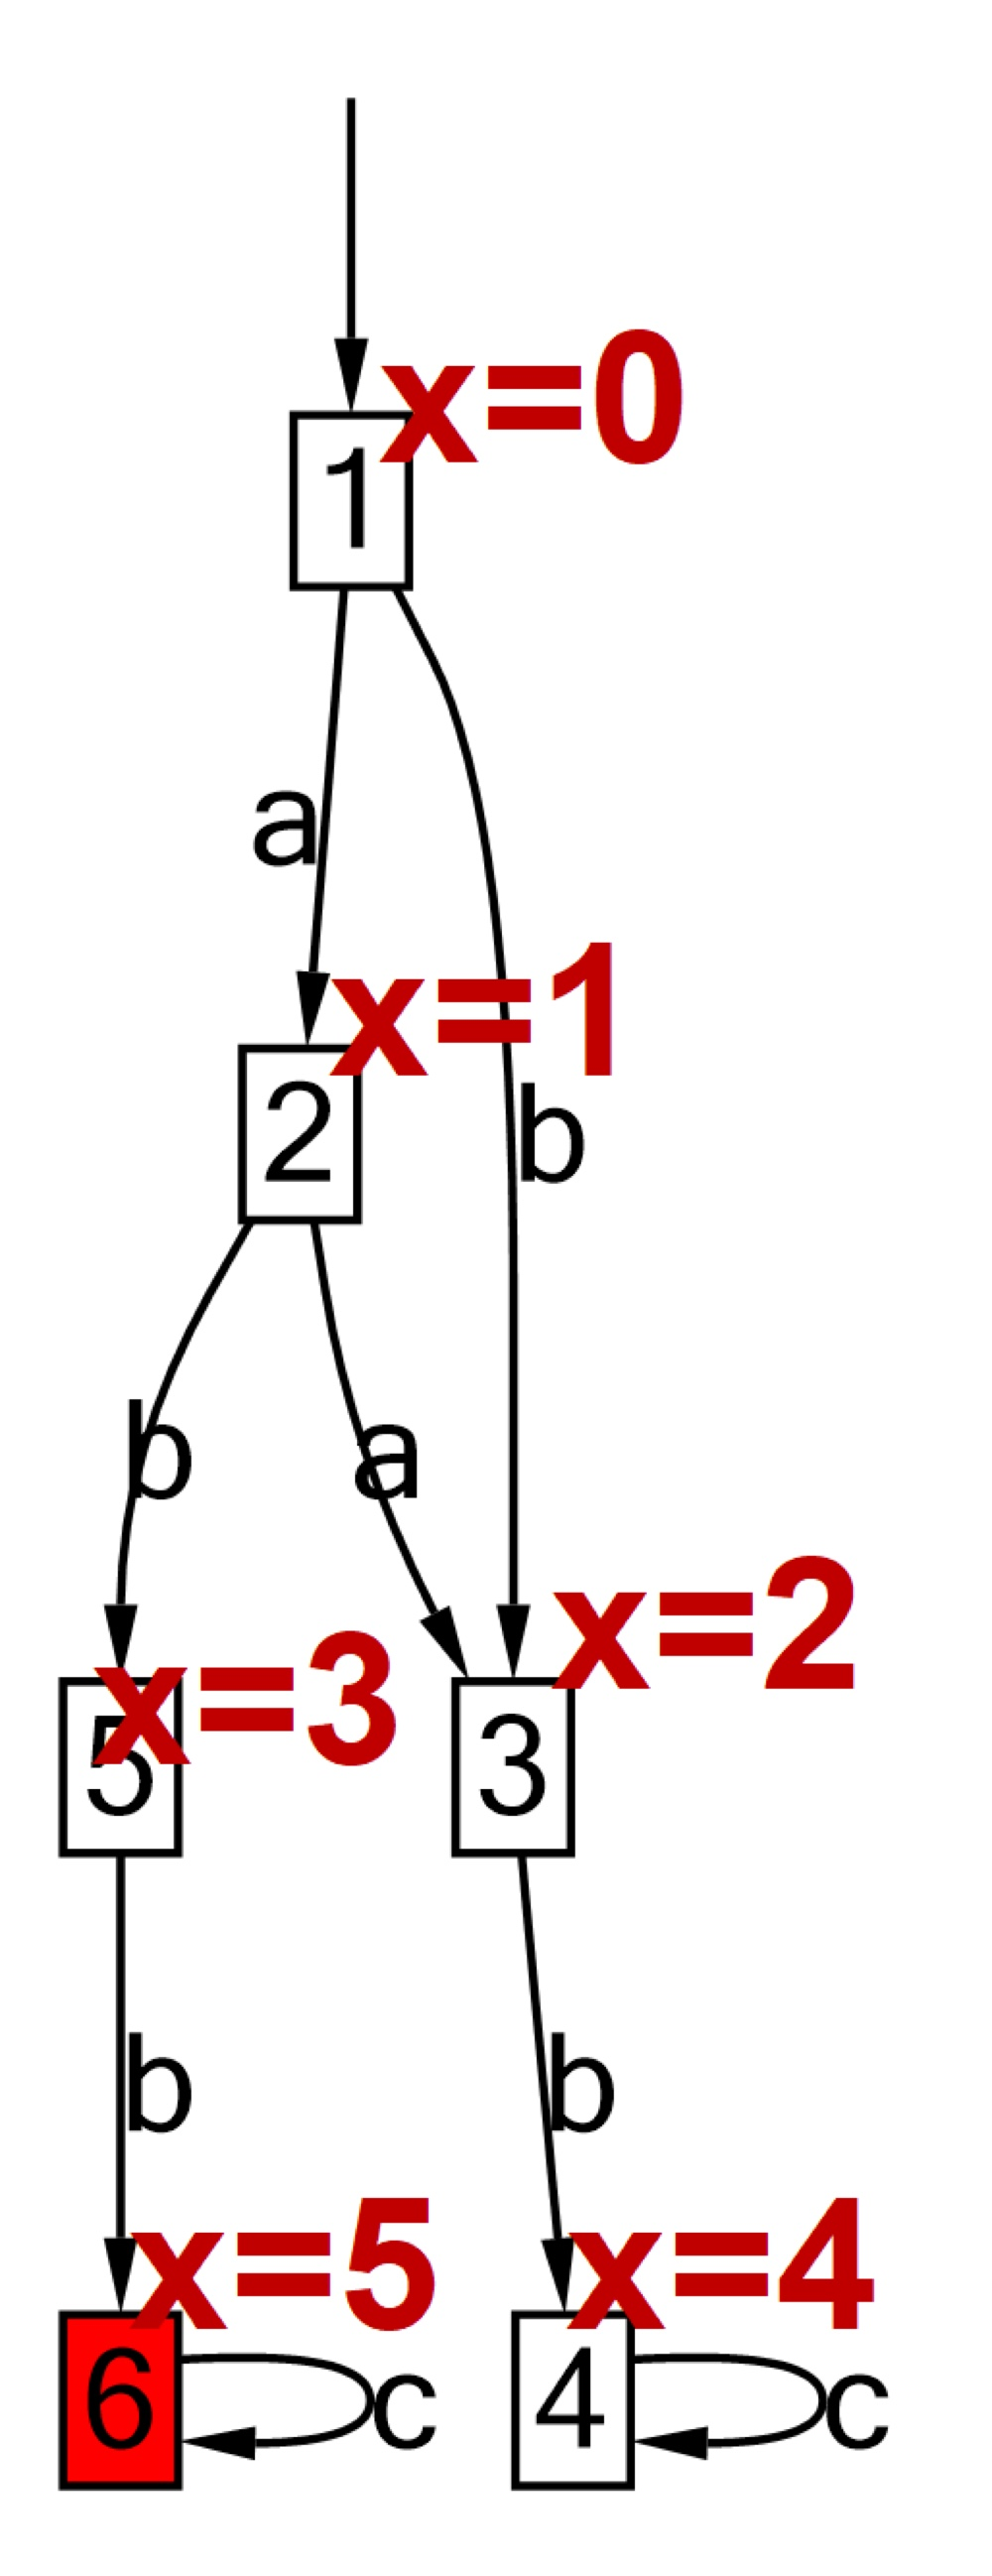
\includegraphics[scale=0.0425]{../images/PAT_Assertions.jpg}
\end{center}
        \end{column}
        \begin{column}{0.55\textwidth}
\begin{lstlisting}[language=C]
#assert P deadlockfree; // Valid

#assert P |= lt2; // First state, x < 2? 
                  // Yes

#assert P |= !c; // Init event is not c? 
                 // Yes

#assert P |= X (a || b); 
// Next event a or b? Yes!

#assert P |= [] ge2; // Always x >= 2? No
// Counter Example: Initial State (x = 0)

#assert P |= <> ge2; // Eventually x >= 2? 
// Yes. Traces: <a, b>, <a, a>, <b>
\end{lstlisting}
        \end{column}
    \end{columns}
\end{frame}

% Slide 116
\begin{frame}[fragile]
    \frametitle{CSP\#: Assertions and Linear Temporal Logic}
    \begin{columns}[t]
        \begin{column}{0.425\textwidth}
\begin{lstlisting}[language=C]
var x = 0;
P = [x < 2] a{x = x + 1} -> P
    [][x < 4] b {x = x + 2} -> P
    [][x >= 4] c -> P;
#define ge2 x >= 2;
#define lt2 x < 2;
\end{lstlisting}
\begin{center}
    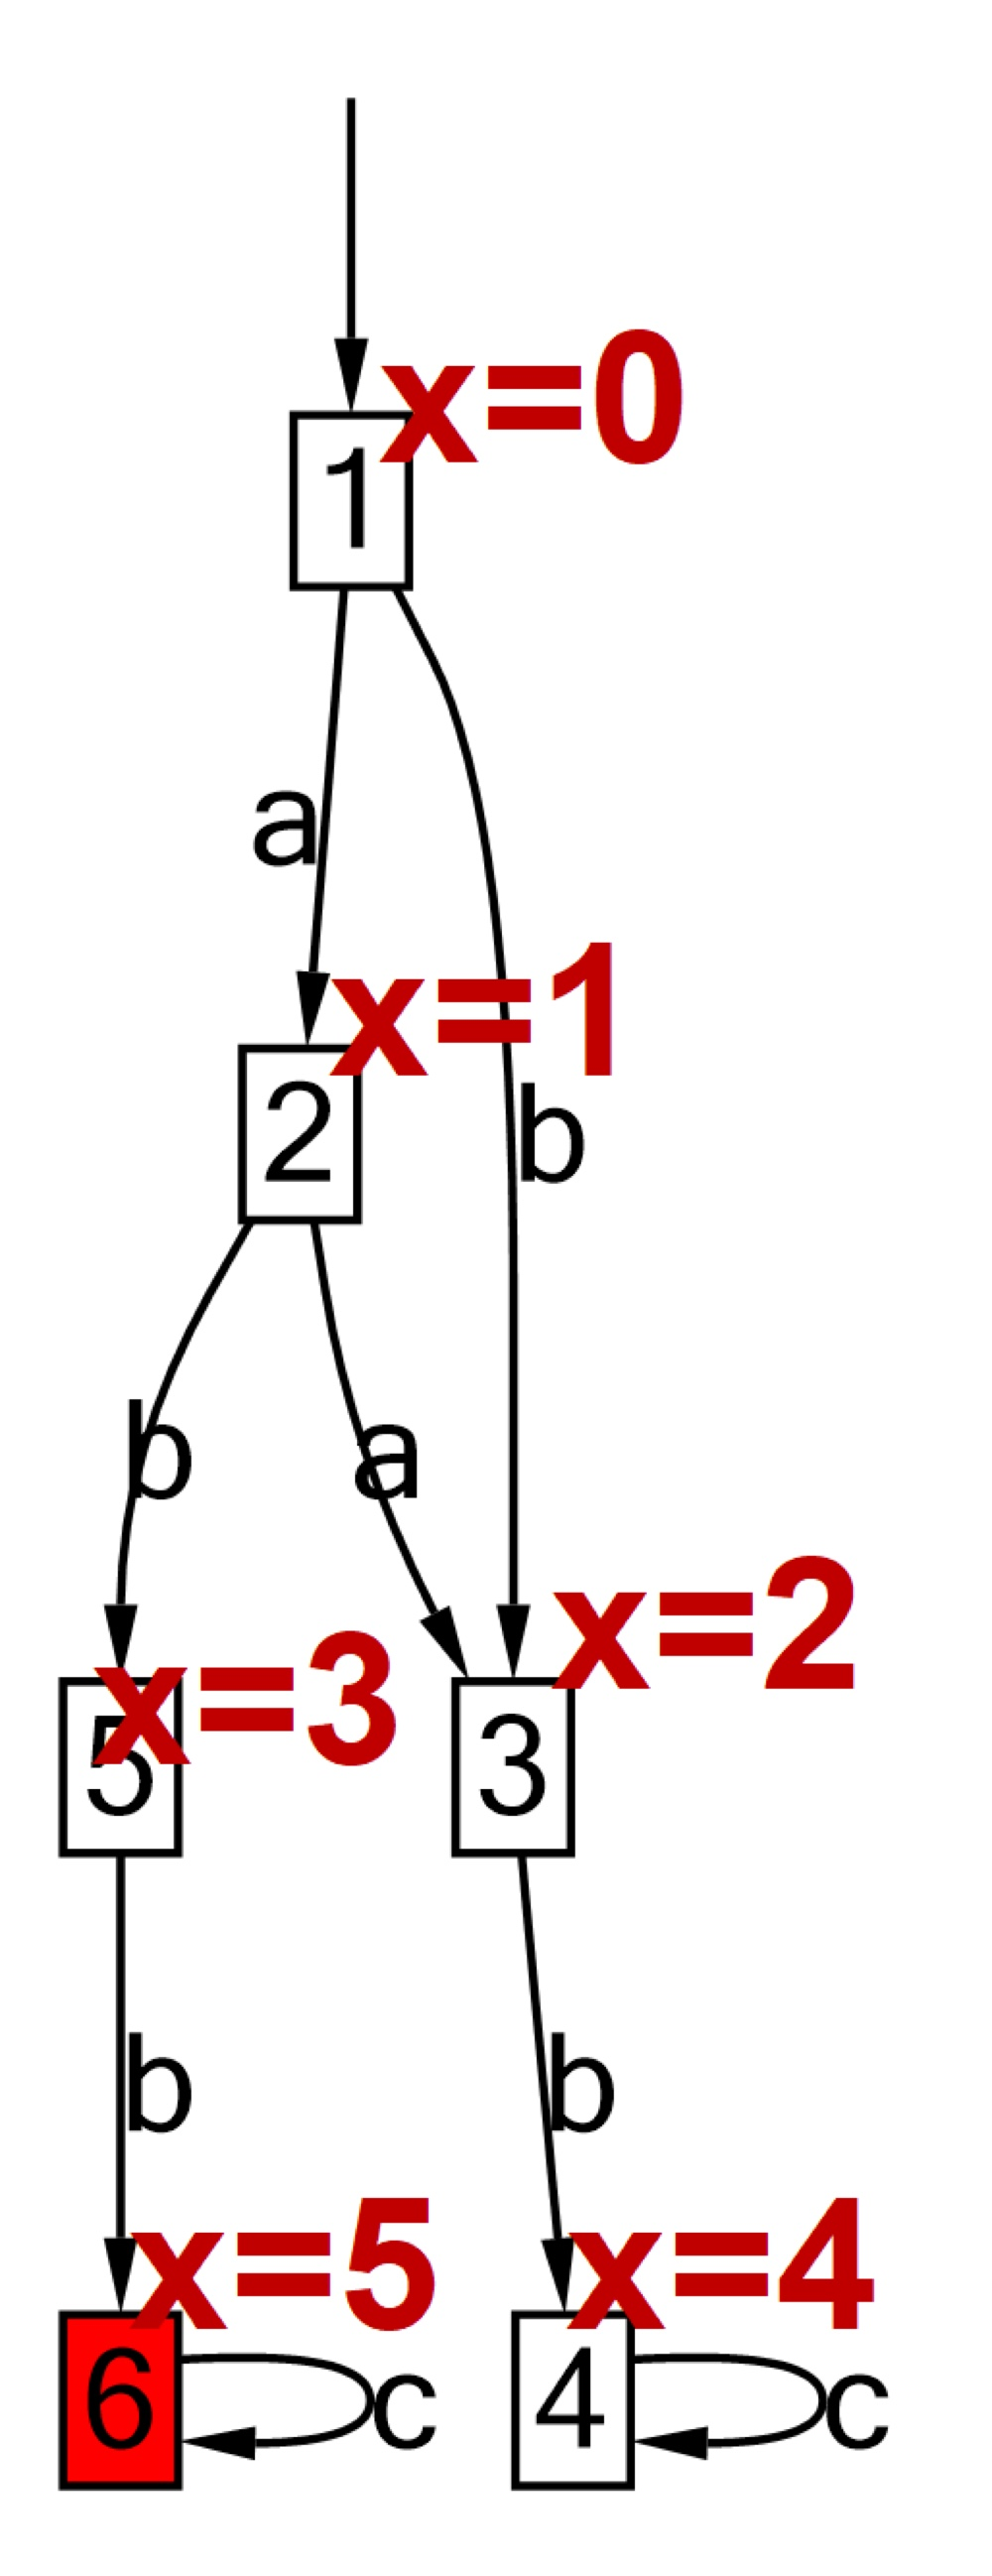
\includegraphics[scale=0.0425]{../images/PAT_Assertions.jpg}
\end{center}
        \end{column}
        \begin{column}{0.55\textwidth}
\begin{lstlisting}[language=C]
#assert P |= [] (lt2 -> X ge2);
// It is always true that if the current state is x < 2, it implies the next state is x >= 2?
// No. For example, <a>, init state x = 0 (lt2), next state x = 1(!ge2)

#assert P |= [] (lt2 -> X(Xge2));
// It is always true that if the current state is x < 2, then the next next state is x >= 2?
// Yes. Traces: <a, a>, <a, b>, <b>
\end{lstlisting}
        \end{column}
    \end{columns}
\end{frame}

% Slide 117
\begin{frame}[fragile]
    \frametitle{CSP\#: Assertions and Linear Temporal Logic}
    \begin{columns}[t]
        \begin{column}{0.425\textwidth}
\begin{lstlisting}[language=C]
var x = 0;
P = [x < 2] a{x = x + 1} -> P
    [][x < 4] b {x = x + 2} -> P
    [][x >= 4] c -> P;
#define ge2 x >= 2;
#define lt2 x < 2;
\end{lstlisting}
\begin{center}
    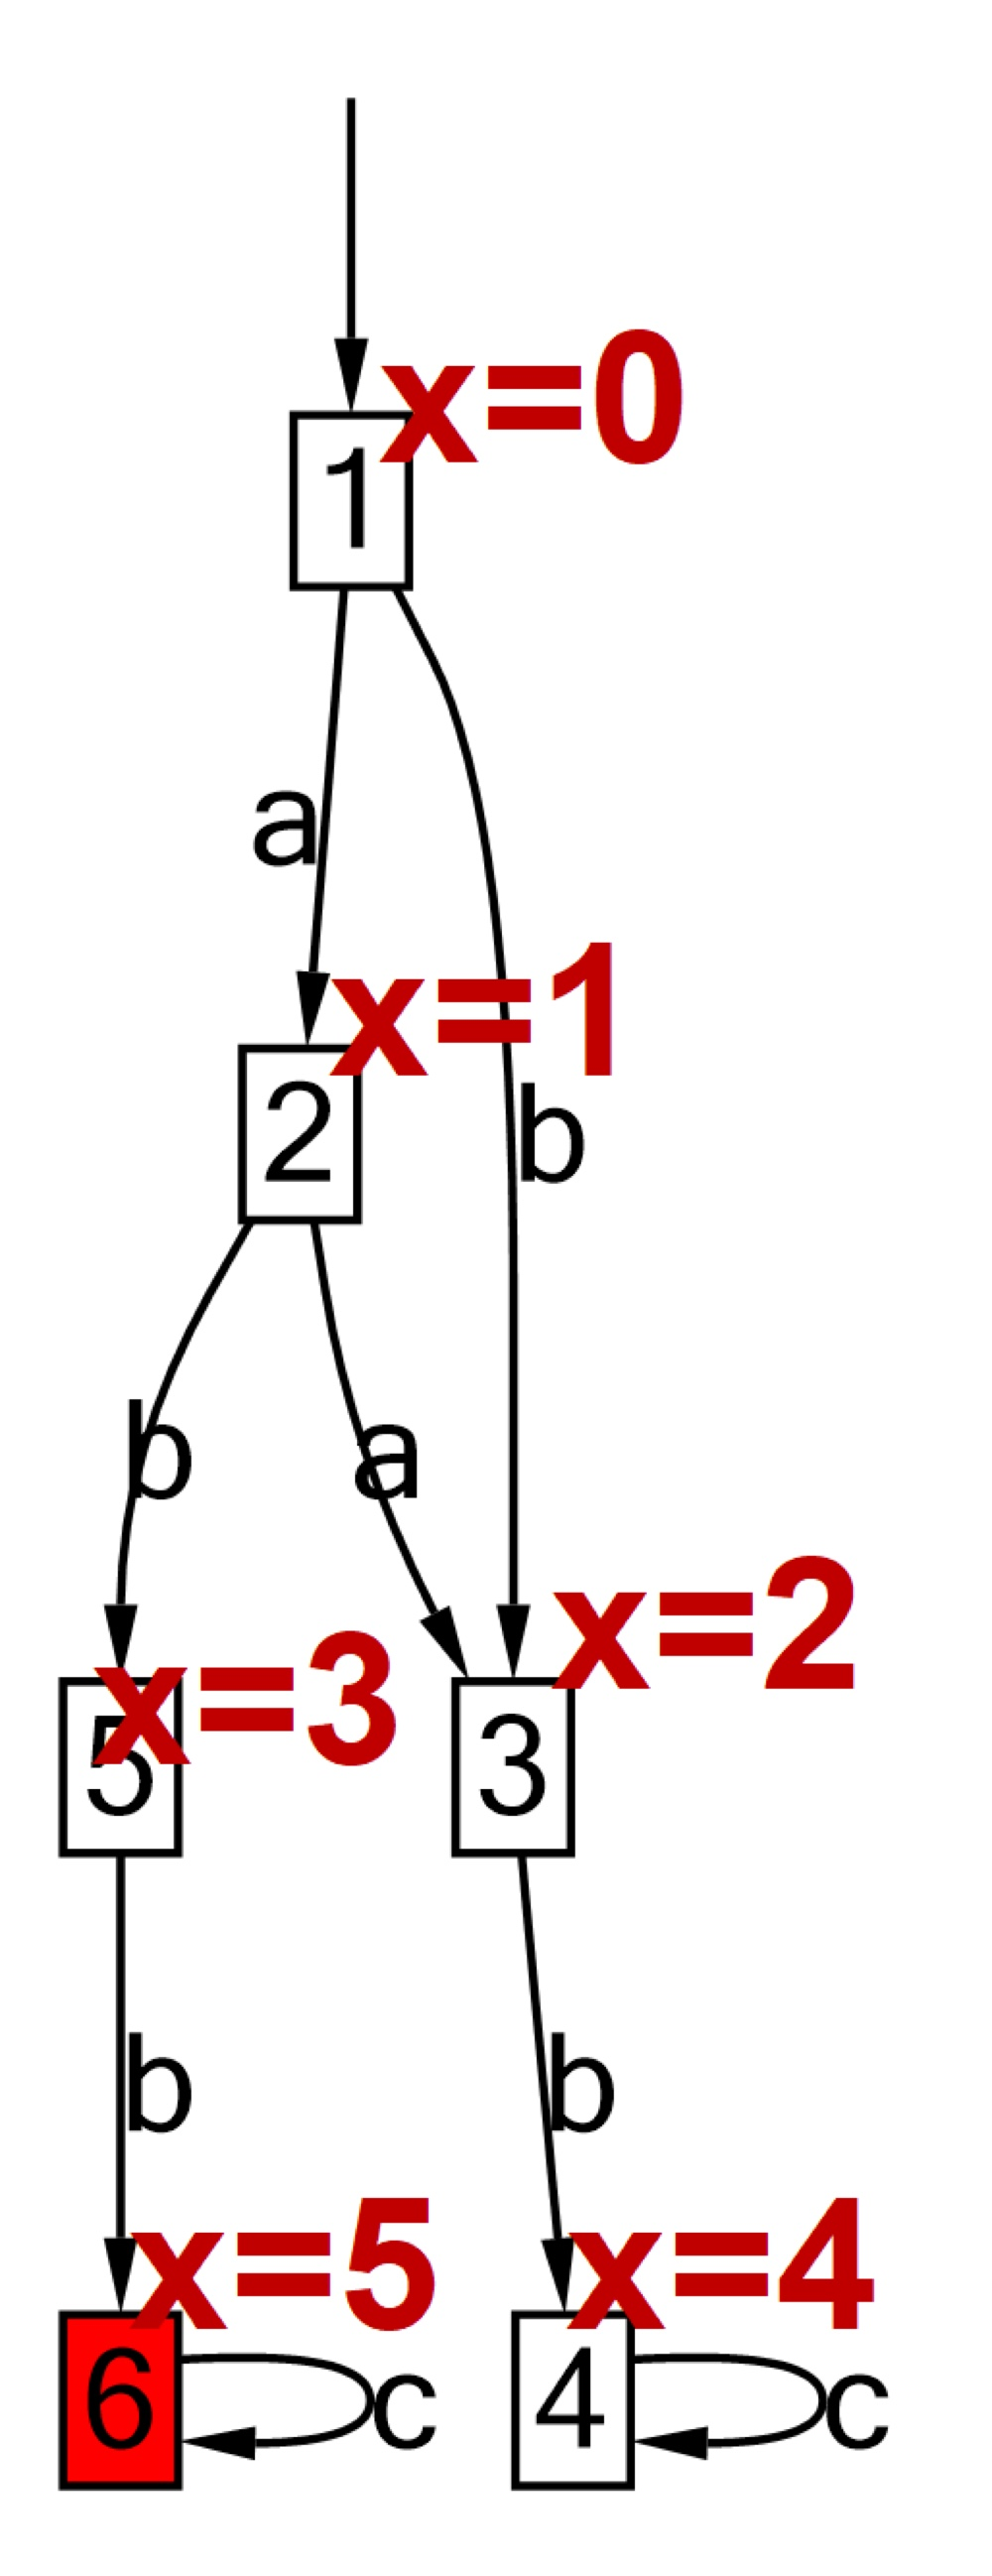
\includegraphics[scale=0.0425]{../images/PAT_Assertions.jpg}
\end{center}
        \end{column}
        \begin{column}{0.55\textwidth}
\begin{lstlisting}[language=C]
#assert P |= (lt2 U ge2); 
// Is it always x < 2 until x >= 2? Yes

#assert P |= (ge2 R le3); 
// x <= 3 until the first position 
// where x >= 2? Yes

#assert P |= (ge2 R lt2); 
// x < 2 until the first position 
// where x >= 2? No
// Counter Examples: <a, b>, <b>
\end{lstlisting}
        \end{column}
    \end{columns}
\end{frame}

% Slide 118
\begin{frame}[fragile]
    \frametitle{CSP\# Example: Patterson's Algorithm}
    Patterson's Algorithm is a concurrent programming algorithm for mutual exclusion that allows two or more processes to share a single-use resource without conflict, using only shared memory for communication.
\begin{lstlisting}[language=C, basicstyle=\scriptsize\selectfont\ttfamily, mathescape]
bool flag[2] = {false, false};
int turn;
\end{lstlisting}
\begin{columns}
\begin{column}{0.475\textwidth}
\begin{lstlisting}[language=C, basicstyle=\scriptsize\selectfont\ttfamily, mathescape]
P0:      flag[0] = true;
P0_gate: turn = 1;
         while (flag[1] && turn == 1) {
            // busy wait
         }
         // critical section
         $\dots$
         // end of critical section
         flag[0] = false;
\end{lstlisting}
\end{column}
\begin{column}{0.5\textwidth}
\begin{lstlisting}[language=C, basicstyle=\scriptsize\selectfont\ttfamily, mathescape]
P1:      flag[1] = true;
P1_gate: turn = 0;
         while (flag[0] && turn == 0) {
             // busy wait
         }
         // critical section
         $\dots$
         // end of critical section
         flag[1] = false;
\end{lstlisting}
\end{column}
\end{columns}
\end{frame}

% Slide 119
\begin{frame}[fragile]
    \frametitle{CSP\# Example: Patterson's Algorithm}
\begin{lstlisting}[language=C, basicstyle=\scriptsize\selectfont\ttfamily, mathescape]
#define N 2;
var pos[N]; // pos[N] is the flag[N]
var step[N]; // step[1] is the !turn
var counter = 0; // how many are in CS

Process0() = Repeat0(1); cs.0{counter = counter + 1;} -> reset{pos[0] = 0; counter = counter - 1;} -> Process0();
Repeat0(j) = [j < N] update.0.1{pos[0] = j;} -> update.0.2{step[j] = 0;} -> ([step[j] != 0 || (pos[1] < j)]idle.j -> Repeat0(j + 1)) 
    [] [j == N] Skip;

Process1() = Repeat1(1); cs.1{counter = counter + 1;} -> reset{pos[1] = 0; counter = counter - 1;} -> Process1();
Repeat1(j) = [j < N] update.1.1{pos[1] = j;} -> update.1.2{step[j] = 1;} -> ([step[j] != 1 || (pos[0] < j)]idle.j -> Repeat1(j + 1)) 
    [] [j == N] Skip;

Peterson() = Process0() ||| Process1();
#define goal counter > 1;
#assert Peterson() reaches goal; // Should be not valid
#assert Peterson() |= <> cs.0; // Should be not valid
#assert Peterson() |= [] (update.0.1 -> <> cs.0) // Should be valid
\end{lstlisting}
\end{frame}

% Slide 120
\begin{frame}{CSP\# Example: Alternating Bit Protocol}
    \begin{itemize}
        \item We are trying to model a simple network protocol that retransmits lost messages between a Sender (A) and Receiver (B).
        \item A sends a bit to B and message may get lost. Using an internal timer, A should retransmit if there is no ACK when {\color{red} \textbf{the time is out}.} A should {\color{orange} \textbf{continue to listen}} for the correct ACK if it receives a wrong one.
        \item B will send ACK if and only if it receives a correct bit. We assume the ACK never gets lost. B should {\color{orange} \textbf{ignore the wrong bit}} received.
        \item After finishing one bit, A and B should move on to send and ACK the alternating bit.
    \end{itemize}
    \begin{block}{Note}
        \texttt{ifa (cond)\{ P \} else \{ Q \};} performs the condition checking and the first operation of P or Q together.
    \end{block}
\end{frame}

% Slide 121
\begin{frame}[fragile]
    \frametitle{CSP\# Example: Alternating Bit Protocol}
\begin{lstlisting}[language=C, basicstyle=\scriptsize\selectfont\ttfamily, mathescape]
channel c 1; // unreliable channel.
channel d 1; // perfect channel.
channel tmr 0; // sender's internal timer.

Sender(alterbit) = (c!alterbit -> Skip [] lost -> Skip); tmr!1 -> Wait4Response(alterbit);

Wait4Response(alterbit) = (d?x -> ifa (x == alterbit) {
    tmr!0 -> Sender(1 - alterbit)
} else { Wait4Response(alterbit) }) // Time not out, wait
[] tmr?2 -> Sender(alterbit); // Time is out, retransmit

Timer = tmr?1 -> (tmr?0 -> Timer [] tmr!2 -> Timer);

Receiver(alterbit) = c?x -> ifa (x == alterbit) {
    d!alterbit -> Receiver(1 - alterbit)
} else { Receiver(alterbit) }; // Wait to receive

ABP = (Sender(0) ||| Receiver(0) ||| Timer);
\end{lstlisting}
\end{frame}

% Slide 122
\begin{frame}[fragile]
    \frametitle{CSP\# Example: Alternating Bit Protocol}
\begin{lstlisting}
#assert ABP |= [](c!0 -> <>d?0);
\end{lstlisting}
Is it always true, that when a Sender process writes 0 into the unreliable channel $c$, a Receiver process will read the value 0 from the perfect channel $d$?
\begin{itemize}
    \item Not valid
    \item Counter Example: $\trace{c!0, c?0, d!0, tmr.1, tmr.2, c!0, c?0, tmr.1, tmr.2, c!0, (c!0, c?0, tmr.1, tmr.2, c!0)^{*}}$
\end{itemize}
\end{frame}

% Slide 123
\begin{frame}[fragile]
    \frametitle{CSP\# Example: Shunting Game}
    Modelling the game board using a 1-D array
\begin{lstlisting}[language=C, basicstyle=\scriptsize\selectfont\ttfamily, mathescape]
#define M 7;
#define N 6;
#define o -1;
#define a 1;
#define w 0;
    // col number: 0 1 2 3 4 5 6
var board[N][M] = [o,o,a,a,o,o,o, // 0 row number starting from 0
                   o,o,a,a,o,o,o, // 1
                   a,a,a,w,a,a,a, // 2
                   a,w,a,a,a,w,a, // 3
                   a,w,a,a,a,w,a, // 4
                   o,o,a,w,o,o,o, // 5
                   o,o,a,a,o,o,o];// 6

// Black Position
var r:{0..N-1} = 3; // row
var c:{0..M-1} = 0; // column
\end{lstlisting}
\end{frame}

% Slide 124
\begin{frame}[fragile]
    \frametitle{CSP\# Example: Shunting Game}
\begin{itemize}
    \item Modelling the moves
\begin{lstlisting}[language=C, basicstyle=\scriptsize\selectfont\ttfamily, mathescape]
Game = [r - 1 >= 0] MoveUp [] [r - 2 >= 0] PushUp
    [] [r + 1 < N] MoveDown [] [r + 2 < N] PushDown
    [] [c - 1 >= 0] MoveLeft [] [c - 2 >= 0] PushLeft
    [] [c + 1 < M] MoveRight [] [c + 2 < M] PushRight;

MoveUp = [board[r - 1][c] == a] go_up{r = r - 1} -> Game;
PushUp = [board[r - 2][c] == a && board[r - 1][c] == w] push_up{
    board[r - 2][c] = w;
    board[r - 1][c] = a;
    r = r - 1;
} -> Game
$\dots$
\end{lstlisting}
    \item Modelling goal and trouble state.
\begin{lstlisting}[language=C, basicstyle=\scriptsize\selectfont\ttfamily, mathescape]
#define goal board[2][2] == w && board[2][3] == w && board[3][2] == w && board[3][3] == w;
#assert Game reaches goal;
#define trouble board[0][3] == w;
#assert Game reaches trouble;
#assert Game |= [](trouble -> ! <> goal); // trouble prevents reaching goal
\end{lstlisting}
\end{itemize}
\end{frame}

% Slide 125
\begin{frame}[fragile]
    \frametitle{CSP\# Example: Keyless System}
    \begin{itemize}
        \item One of the latest automotive technologies, a push-button keyless system, allows you to start your car's engine without the hassle of key insertion and offers great convenience.
        \item These systems are designed so it is possible to start the engine without the owner's key-fob and it cannot lock your key fob inside the car because the system will sense it and prevent the user from locking them in.
        \item \color{red} However, the keyless system can also suprise you as it may allow you to drive the car without a key-fob, meaning you can drive without physically having the key.
        \item In this example, we will model such a Keyless System and use assertions to check if one can drive the car without having a key with them.
    \end{itemize}
\begin{lstlisting}[language=C, basicstyle=\scriptsize\selectfont\ttfamily, mathescape]
\end{lstlisting}
\end{frame}

% Slide 126
\begin{frame}[fragile]
    \frametitle{CSP\# Example: Keyless System}
Constants and variables
\begin{lstlisting}[language=C, basicstyle=\scriptsize\selectfont\ttfamily, mathescape]
#define N 2; // number of owners
#define far 0; // owner is out and far away from the car
#define near 1; // owner is close enough to open / lock the car if he has the keyfob
#define in 2; // owner is in the car
#define off 0; // engine is off
#define on 1; // engine is on
#define unlock 0; // door is unlocked but closed
#define lock 1; // door is locked (and must be closed)
#define open 2; // door is open
#define incar -1; // keyfob is put inside car
#define faralone -2; // keyfob is put outside and far

var owner[N]; // owners' position, initially all users are far away from the car
var engine = off; // engine status, intially off
var door = lock; // door status, initally locked
var key = 0; // key fob position, initially with its first owner
var moving = 0; // car moving status, 0 for stop and 1 for moving
var fuel = 10; // energy costs, say 1 for a short drive and 5 for long driving
\end{lstlisting}
\end{frame}

% Slide 127
\begin{frame}[fragile]
    \frametitle{CSP\# Example: Keyless System}
\begin{itemize}
    \item Owner positions
\begin{lstlisting}[language=C, basicstyle=\scriptsize\selectfont\ttfamily, mathescape]
car = (||i:{0..N-1} @ (owner_pos(i) || motor(i) || door_op(i) || key_pos(i)));

owner_pos(i) = [owner[i] == far] towards.i{owner[i] = near} -> owner_pos(i)
            [] [owner[i] == near] goaway.i{owner[i] = far} -> owner_pos(i)
            [] [owner[i] == near && door == open && moving == 0] 
                getin.i{owner[i] = in} -> owner_pos(i)
            [] [owner[i] == in && door == open && moving == 0] 
            goout.i{owner[i] = near} -> owner_pos(i);
\end{lstlisting}
    \item Key-fob positions
\begin{lstlisting}[language=C, basicstyle=\scriptsize\selectfont\ttfamily, mathescape]
key_pos(i) = 
    [key == i && owner[i] == in] putincar.i{key = incar} -> key_pos(i)
 [] [key == i && owner[i] == far] putaway.i{key = faralone} -> key_pos(i)
 [] [(key == faralone && owner[i] == far) || (key == incar && owner[i] == in)] getkey.i{key = i} -> key_pos(i);

\end{lstlisting}
\end{itemize}
\end{frame}

% Slide 128
\begin{frame}[fragile]
    \frametitle{CSP\# Example: Keyless System}
Door Operation
\begin{lstlisting}[language=C, basicstyle=\scriptsize\selectfont\ttfamily, mathescape]
door_op(i) =
    [key == i && owner[i] == near && door == lock && moving == 0] 
    unlockopen.i{door = open} -> door_op(i)
 [] [owner[i] == near && door == unlock && moving == 0] justopen.i{door = open} -> door_op(i)
 [] [door != open && owner[i] == in] insideopen.i{door = open} -> door_op(i)
 [] [door == open] close.i{door = unlock} -> door_op(i)
 [] [door == unlock && owner[i] == in] insidelock.i{door = lock} -> door_op(i)
 [] [door == unlock && owner[i] == near && key == i] outsidelock.i{door = lock} -> door_op(i);
\end{lstlisting}
\end{frame}

% Slide 129
\begin{frame}[fragile]
    \frametitle{CSP\# Example: Keyless System}
Motor
\begin{lstlisting}[language=C, basicstyle=\scriptsize\selectfont\ttfamily, mathescape]
motor(i) =
    [owner[i] == in && (key == i || key == incar) && engine == off && fuel != 0] turnon.i{engine = on} -> motor(i)
 [] [engine == on && owner[i] == in && moving == 0] startdrive.i{
        moving = 1;
    } -> motor(i)
 [] [moving == 1 && fuel != 0] shortdrive.i{
        fuel = fuel - 1; 
        if (fuel == 0) {engine = off; moving = 0;}
    } -> motor(i)
 [] [moving == 1 && fuel > 5] longdrive.i{
        fuel = fuel - 5; 
        if (fuel == 0) { engine = off; moving = 0; }
    } -> motor(i)
 [] [engine == on && moving == 1 && owner[i] == in] stop.i{moving = 0;} -> motor(i)
 [] [fuel == 0 && engine == off] refill{fuel = 10} -> motor(i)
 [] [engine == on && moving == 0 && owner[i] == in] turnoff.i{
        engine = off;
    } -> motor(i);
\end{lstlisting}
\end{frame}

% Slide 130
\begin{frame}[fragile]
    \frametitle{CSP\# Example: Keyless System}
Reasoning
\begin{lstlisting}[language=C, basicstyle=\scriptsize\selectfont\ttfamily, mathescape]
#define keylockinside (key == incar && door == lock && owner[0] != in && owner[1] != in);
#define drivewithoutengineon (moving == 1 && engine == off);
#define drivewithoutkeyholdbyother (moving == 1 && owner[1] == in && owner[0] == far && key == 0);

#assert car deadlockfree;
#assert car reaches keylockinside; // False
#assert car reaches drivewithoutengineon; // False
#assert car reaches drivewithoutkeyholdbyother; // True
\end{lstlisting}
\end{frame}

% Slide 131
\begin{frame}[fragile]
    \frametitle{CSP\# Example: Multi-lift System (using C\#)}
    In this example, we are modelling a multiple lift system in a building with multiple floors.

\begin{lstlisting}[language=C, basicstyle=\scriptsize\selectfont\ttfamily, mathescape]
#define NoOfFloors 2; // floor-0, floor-1
#define NoOfLifts 2; // lift-0, lift-1
#define NoOfUsers 2; // user-0, user-1

// this array models the external requests; extrequestsUP[i] = 1 denotes there is an upward floor request at floor-i; 0 for no request;
var extrequestsUP[NoOfFloors];
var extrequestsDOWN[NoOfFloors];
// this array models the internal requests;
// intrequests[i][j] = 1 if there is a request for floor-i for lift-j; 0 for no request;
var intrequests[NoOfLifts][NoOfFloors]; // [-1, -1]

// the level of the lift door opens at. -1 means the door is closed
var door = [-1(NoOfLifts)];
\end{lstlisting}
\end{frame}

% Slide 132
\begin{frame}[fragile]
    \frametitle{CSP\# Example: Multi-lift System (using C\#)}
    Data Operations to clear internal and external requests when the door of the lift-i is open at each level.

\begin{lstlisting}[language=C, basicstyle=\scriptsize\selectfont\ttfamily, mathescape]
door[i] = level;
intrequests[i][level] = 0;
if (direction > 0) {
    extrequestsUP[level] = 0;
} else {
    extrequestsDOWN[level] = 0;
}
\end{lstlisting}
\end{frame}

% Slide 133
\begin{frame}[fragile]
    \frametitle{CSP\# Example: Multi-lift System (using C\#)}
    Data Operations (using a function defined in an external C\# library) to check whether to continue travelling on the same direction or to change direction.

\begin{lstlisting}[language=C, basicstyle=\scriptsize\selectfont\ttfamily, mathescape]
public static bool CheckIfToMove(int level, int direction, int i, int NoOfFloors, int[] intrequests, int[] extrequestsUP, int[] extrequestsDOWN) {
    int Counter = level + direction;
    while (Counter >= 0 && Counter < NoOfFloors) {
        if (extrequestsUP[Counter] != 0 || extrequestsDOWN[Counter] != 0 || intrequests[i * NoOfFloors + Counter] != 0) {
            return true;
        } else {
            Counter = Counter + direction;
        }
    }
    return false;
}
\end{lstlisting}
\end{frame}

% Slide 134
\begin{frame}[fragile]
    \frametitle{CSP\# Example: Multi-lift System (using C\#) Modelling the Lift}
\begin{lstlisting}[language=C, basicstyle=\scriptsize\selectfont\ttfamily, mathescape]
Lift(i, level, direction) = ifa(intrequests[i][level] != 0 || (direction == 1 && extrequestsUP[level] == 1) || (direction == -1 && extrequestsDOWN[level] == 1)) {
    opendoor.i.level{ *data operations to clear request* } -> close.i.level{door[i] = -1;} -> Lift(i, level direction)
} else {
    checkIfToMove.i.level -> ifa(call(CheckIfToMove, level, direction, i, 
    NoOfFloors, intrequests, extrequestsUP, extrequestsDOWN)) {
        moving.i.level.direction -> 
        ifa (level + direction == 0 || level + direction == NoOfFloors - 1) {
            Lift(i, level + direction, -1 * direction)
        } else {
            Lift(i, level + direction, direction)
        }
    } else {
        ifa ((level == 0 && direction == 1) || 
             (level == NoOfFloors - 1 && direction == -1)) {
            Lift(i, level, direction)
        } else {
            changedir.i.level -> Lift(i, level, -1 * direction)
        }
    }
}
\end{lstlisting}
\end{frame}

% Slide 135
\begin{frame}[fragile]
    \frametitle{CSP\# Example: Multi-lift System (using C\#) Modelling the Users}
\begin{lstlisting}[language=C, basicstyle=\scriptsize\selectfont\ttfamily, mathescape]
User() = []pos:{0..NoOfFloors - 1}@ (ExternalPush(pos); UserWaiting(pos));

// The following models the behaviours of the user pushing external buttons
ExternalPush(pos) = ifa(pos != 0) {pushdown.pos{extrequestsDOWN[pos] = 1;} -> Skip} 
                    else {pushup.pos{extrequestsUP[pos] = 1;} -> Skip} 
[] ifa(pos != NoOfFloors - 1) {pushup.pos{extrequestsUP[pos] = 1;} -> Skip} 
    else {pushdown.pos{extrequestsDOWN[pos] = 1;} -> Skip};

// The following models the behaviours of the user waiting and entering the lift
UserWaiting(pos) = []i:{0..NoOfLifts - 1}@([door[i] == pos]enter.i -> 
    ([]y:{0..NoOfFloors - 1}@push.y{intrequests[i][y] = 1;} -> 
        ([door[i] == y]exit.i -> User())));
\end{lstlisting}
\end{frame}

% Slide 136
\begin{frame}[fragile]
    \frametitle{CSP\# Example: Multi-lift System (using C\#) Questioning the System}
\begin{lstlisting}[language=C, basicstyle=\scriptsize\selectfont\ttfamily, mathescape]
// A Lift System consisting of multiple users and lifts running in parallel
LiftSystem() = (||| {NoOfUsers} @ User()) ||| 
    (||| x:{0..NoOfLifts - 1} @ Lift(x, 0, 1));

// If there is an external request at the first floor, it will eventually be served.
#define on extrequestsUP[0] == 1;
#define off extrequestsUP[0] == 0;
#assert LiftSystem() |= [](on -> <>off);
\end{lstlisting}
\end{frame}

% Slide 137
\begin{frame}[fragile]
    \frametitle{CSP\# Example: 2-phase Commit Protocol}
\begin{lstlisting}[language=C, basicstyle=\scriptsize\selectfont\ttfamily, mathescape]
#define N 2; // number of participants
enum {Yes, No, Commit, Abort}; // constants
channel vote 0;
var hasNo = false;

// The following models the coordinator
Coord() = (|||{N}@ request -> Skip); 
          (|||{N}@ vote?vo{if (vo == No) {hasNo = true;}} -> Skip);
          decide -> (([hasNo == false] (|||{N}@inform.Commit -> Skip); 
          CoordPhaseTwo(Commit))
          [] ([hasNo == true] (|||{N}@inform.Abort -> Skip); CoordPhaseTwo(Abort)));
CoordPhaseTwo(decC) = |||{N}@acknowledge -> Skip;

// The following models a participant
Part() = request -> execute -> (vote!Yes -> PhaseTwo() [] vote!No -> PhaseTwo());
PhaseTwo() = inform.Commit -> complete -> result.Commit -> acknowledge -> Skip 
           [] inform.Abort -> undo -> result.Abort -> acknowledge -> Skip;

#alphabet Coord {request, inform.Commit, inform.Abort, acknowledge};
#alphabet Part {request, inform.Commit, inform.Abort, acknowledge};
System = Coord() || (|||{N}@Part()); // Note: request is a common event between Coord and Part and has to be synchronised.
\end{lstlisting}
\end{frame}

% Slide 138
\section{Timed and Probability CSP}

% Slide 139
\begin{frame}[fragile]
    \frametitle{Real-Time System (RTS) Module}
    \begin{itemize}
        \item The Real-Time System (RTS) module is an extension of the CSP module with operators which captures quantitative \textbf{timing requirements.}
        \item Let $P$ and $Q$ be processes, while $d$ represents a duration of $d$ time units.
    \end{itemize}
\begin{lstlisting}[language=C]
P = Wait[t] // delay
P = P timeout[t] Q // timeout
P = P interrupt[t] Q // timed interrupt
P = P deadline [t] // deadline
P = P within[t] // within
\end{lstlisting}
\end{frame}

% Slide 140
\begin{frame}[fragile]
    \frametitle{Timed Process Definition: Wait}
    \begin{itemize}
        \item A wait process \texttt{Wait[t]} delays the system execution for a period of t time units then terminates.
        \item In the subsequent slides, a set of inference rules using premises and conclusions will be used to define the behaviour of each timed process.
        \item Recall that each (V, P) is an ordered pair of values and processes.
    \end{itemize}
    \begin{columns}[t]
        \begin{column}{0.5\textwidth}
            \begin{small}
                \textbf{Definition 1}
                \begin{axdef}
                    t \leq d
                    \where
                    (V, Wait[d]) \xrightarrow{t} (V, Wait[d - t])
                \end{axdef}

                \textbf{Definition 2}
                \begin{axdef}
                    \where
                    (V, Wait[0]) \xrightarrow{\tau} (V, Skip)
                \end{axdef}
            \end{small}
        \end{column}
        \begin{column}{0.5\textwidth}
\begin{lstlisting}[language=C]
P = Wait[t]; P
\end{lstlisting}
        \begin{itemize}
            \item The starting time of process P is delayed by exactly t time units.
            \item If the amount of time elapsed is less than the specified duration, then the Wait process will be still active.
        \end{itemize}
        \end{column}
    \end{columns}
\end{frame}

% Slide 141
\begin{frame}[fragile]
    \frametitle{Timed Process Definition: Wait (Example)}
    \begin{columns}
        \begin{column}{0.5\textwidth}
\begin{lstlisting}[language=C]
P = Wait[2]; (a -> b -> Skip);
\end{lstlisting}
            \begin{itemize}
                \item The Wait process is active for exactly 2 time units.
                \item In this example, the first event \textbf{a} begins only at least after 2 time units.
            \end{itemize}
        \end{column}
        \begin{column}{0.475\textwidth}
            \begin{center}
                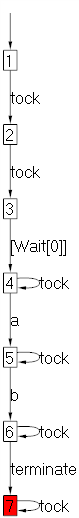
\includegraphics[scale=0.5]{../images/L4_WaitExample.JPG}
            \end{center}
        \end{column}
    \end{columns}
\end{frame}

% Slide 142
\begin{frame}[fragile]
    \frametitle{Timed Process Definition: Timeout}
    
    \begin{itemize}
        \item The process \texttt{P timeout[t] Q} passes control to process \texttt{Q} if no event has occured in process \texttt{P} before t time units have elapsed.
        \item For instance if process \texttt{a -> P timeout [t] Q} engages in event \texttt{a} before $t$ time units have elapsed since the process is enabled, then the process is transformed to P.
        \item If event \texttt{a} has not occured by time $t$, the process transforms to Q (by silent tau-transition).
    \end{itemize}
    \begin{block}{Invisible Events}
        \begin{enumerate}
            \item Let $\tau$ (tau) be an invisible event. Example: \texttt{tau\{pv = x\}}
            \item \texttt\{ pv = x \} (Event with no name is also an invisible event)
        \end{enumerate}
        \textbf{Note:} Invisible events are not observable.
    \end{block} 
\end{frame}

% Slide 143
\begin{frame}{Timed Process Definition: Timeout}
    \begin{small}
        \begin{itemize}
            \item The timeout constraint is removed if an event in P is engaged before $d$ time units has elapsed.
            \begin{footnotesize}
                \begin{axdef}
                    (V, P) \xrightarrow{x} (V', P')
                    \where
                    (V, \text{$P$ timeout[d] $Q$}) \xrightarrow{x} (V', P')
                \end{axdef}
            \end{footnotesize}
            \item If P engages in an invisible event $\tau$, the timeout constraint is not removed, but the process becomes \texttt{P' timeout[d] Q}
            \begin{footnotesize}
            \begin{axdef}
                (V, P) \xrightarrow{\tau} (V, P')
                \where
                (V, \text{$P$ timeout[d] $Q$}) \xrightarrow{\tau} (V', \text{P' timeout[d] $Q$})
            \end{axdef}
            \end{footnotesize}
            \item If time has not passed d units, the timeout constraint remains.
            \begin{footnotesize}
                \begin{axdef}
                    (V, P) \xrightarrow{t} (V, P'), t \leq d
                    \where
                    (V, \text{$P$ timeout[d] $Q$}) \xrightarrow{t} (V, \text{P' timeout[d - t] $Q$})
                \end{axdef}
            \end{footnotesize}
            \item If no event has occured by timeout, the process transforms to Q by silent-tau transition.
            \begin{footnotesize}
                \begin{axdef}
                    \where
                    (V, \text{$P$ timeout[0] $Q$}) \xrightarrow{\tau} (V, Q)
                \end{axdef}
            \end{footnotesize}
        \end{itemize}
    \end{small}
\end{frame}

% Slide 144
\begin{frame}[fragile]
    \frametitle{Timed Process Definition: Timeout (Example)}
\begin{columns}
    \begin{column}{0.6\textwidth}
\begin{lstlisting}[language=C]
P = (a -> b -> Skip) timeout[2] (e -> Skip);
\end{lstlisting}
        \begin{itemize}
            \item As long as process P engages event \textbf{a} within 2 time units and before \texttt{timeout[0]} is engaged, the timeout constrained is removed and \texttt{(e -> Skip)} will never be engaged.
            \item \texttt{(e -> Skip)} can only be engaged after \texttt{timeout[0]} is engaged.
        \end{itemize}
    \end{column}
    \begin{column}{0.375\textwidth}
        \begin{center}
            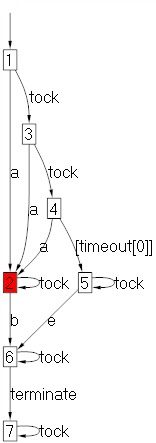
\includegraphics[scale=0.5]{../images/L4_TimeoutExample.JPG}
        \end{center}
    \end{column}
\end{columns}
\end{frame}

% Slide 145
\begin{frame}{Timed Process Definition: Timed Interrupt}
    \begin{itemize}
        \item Process \texttt{P interrupt[t] Q} behaves as P until t time unit elapse and then switches to Q
        \item For example process \texttt{(a -> b -> c -> \dots) interrupt[t] Q} may engage in events a, b, c, \dots as long as $t$ time units has not elapsed.
        \item Once t time units have elapse, then the process transforms to Q by silent-tau transition.
    \end{itemize}

    \textbf{Definition 1}
    \begin{footnotesize}
        \begin{axdef}
            (V, P) \xrightarrow{x} (V', P')
            \where
            (V, \text{$P$ interrupt[d] $Q$}) \xrightarrow{x} (V', \text{$P'$ interrupt[d] $Q$})
        \end{axdef}
    \end{footnotesize}

    \textbf{Definition 2}
    \begin{footnotesize}
        \begin{axdef}
            (V, P) \xrightarrow{t} (V', P'), t \leq d
            \where
            (V, \text{$P$ interrupt[d] $Q$}) \xrightarrow{t} (V', \text{$P'$ interrupt[d - t] $Q$})
        \end{axdef}
    \end{footnotesize}

    \textbf{Definition 3}
    \begin{footnotesize}
        \begin{axdef}
            \where
            (V, \text{$P$ interrupt[0] $Q$}) \xrightarrow{\tau} (V', Q)
        \end{axdef}
    \end{footnotesize}
\end{frame}

% Slide 146
\begin{frame}[fragile]
    \frametitle{Timed Process Definition: Timed Interrupt (Example)}
\begin{columns}
    \begin{column}{0.6\textwidth}
\begin{lstlisting}[language=C]
P = (a -> b -> Skip) interrupt[2] (e -> Skip);
\end{lstlisting}
        \begin{itemize}
            \item Process P can engage in the events in \texttt{(a -> b -> Skip)} until 2 time unit has elapsed.
            \item After 2 time units has elapsed, Process P can only engage in events in \texttt{(e -> Skip)}.
        \end{itemize}
    \end{column}
    \begin{column}{0.375\textwidth}
        \begin{center}
            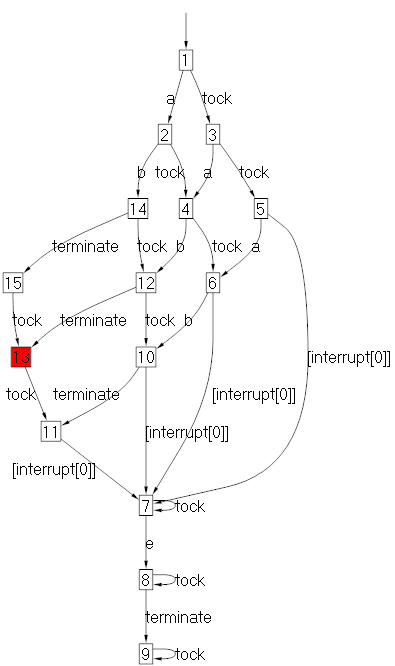
\includegraphics[scale=0.4]{../images/L4_TimedInterruptExample.JPG}
        \end{center}
    \end{column}
\end{columns}
\end{frame}

% Slide 147
\begin{frame}[fragile]
    \frametitle{Timed Process Definition: Deadline}
Process \texttt{P deadline[t]} is constrained to terminate within $t$ time units.

\begin{columns}
    \begin{column}{0.525\textwidth}
        \textbf{Definition 1}
        \begin{footnotesize}
            \begin{axdef}
                (V, P) \xrightarrow{x} (V', P')
                \where
                (V, \text{$P$ deadline[d]}) \xrightarrow{x} (V', \text{$P'$ deadline[d]})
            \end{axdef}
        \end{footnotesize}

        \textbf{Definition 2}
        \begin{footnotesize}
            \begin{axdef}
                (V, P) \xrightarrow{t} (V', P'), t \leq d
                \where
                (V, \text{$P$ deadline[d]}) \xrightarrow{t} (V', \text{$P'$ deadline[d - t]})
            \end{axdef}
        \end{footnotesize}

        \textbf{Definition 3}
        \begin{footnotesize}
            \begin{axdef}
                \where
                (V, \text{$P$ interrupt[0]}) \rightarrow Skip
            \end{axdef}
        \end{footnotesize}
    \end{column}
    \begin{column}{0.45\textwidth}
        \begin{center}
            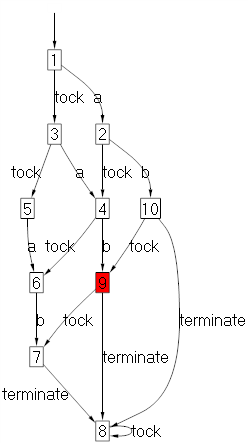
\includegraphics[scale=0.45]{../images/L4_DeadlineExample.JPG}
        \end{center}
\begin{lstlisting}[language=C]
P = (a -> b -> Skip) deadline[2];
\end{lstlisting}
    \end{column}
\end{columns}
\end{frame}

% Slide 148
\begin{frame}[fragile]
    \frametitle{Timed Process Definition: Within}
    \begin{columns}
        \begin{column}{0.75\textwidth}
            \begin{itemize}
                \item The within operator forces the process to make an observable move within the given time frame.
                \item For example \texttt{P within[t]} says the first event of P must engage within $t$ time units.
                \item In the example below, event a has to be engaged by latest $t = 2$ which is at \textbf{State 4}.
            \end{itemize}
\begin{lstlisting}[language=C]
P = (a -> b -> Skip) within[2];
\end{lstlisting}
        \end{column}
        \begin{column}{0.2\textwidth}
            \begin{center}
                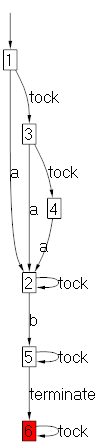
\includegraphics[scale=0.55]{../images/within_operator.JPG}
            \end{center}
        \end{column}
    \end{columns}
\end{frame}

% Slide 149
\begin{frame}[fragile]
    \frametitle{CSP\# Example: Fischer's Protocol}
    Mutual exclusion in Fischer's Protocol is guaranteed by carefully placing bounds on the execution times of the instructions, leading to a protocol which is very simple, and relies heavily on time aspects.
\begin{lstlisting}[language=C]
#define N 2;
#define Delta 3;
#define Epsilon 4;
#define Idle -1;
var x = Idle;
var counter;

P(i) = ifb(x == Idle) {
    ((update.i{x = i} -> Wait[Epsilon]) within[Delta]);
    ([x == i](cs.i{counter++} -> exit.i{counter--; x=Idle} -> P(i))
    [] [x != i]P(i))
};

FischersProtocol = ||| i:{0..N-1}@P(i);
\end{lstlisting}
\end{frame}

% Slide 150
\begin{frame}[fragile]
    \frametitle{CSP\# Example: Railway Crossing System}
    Control trains passing a critical point (a bridge)
\begin{scriptsize}
\begin{lstlisting}[language=C, basicstyle=\scriptsize\selectfont\ttfamily]
#import "PAT.Lib.Queue";
#define N 2;
channel appr 0;
channel go 0;
channel leave 0;
channel stop 0;
var<Queue> queue;

Train(i) = appr!i -> ((stop?i -> StopS(i) within[10]) timeout[10] Cross(i));
Cross(i) = Wait[4]; (leave!i -> Train(i)) within[11];
StopS(i) = go?i -> Start(i);
Start(i) = Wait[10]; (leave!i -> Train(i)) within[10];
Gate = if (queue.Count() ==0) {
    appr?i -> atomic{tau{queue.Enqueue(i)} -> Skip}; Occ 
} else {
    (go!queue.First() -> Occ) within[10] 
};

Occ = (leave?[i == queue.First()]i -> atomic{tau{queue.Dequeue()} -> Skip}; Gate) [] (appr?i -> atomic{tau{queue.Enqueue(i)} -> stop!queue.Last() -> Skip}; Occ);
System = (||| x:{0..N-1}@Train(x)) ||| Gate;
\end{lstlisting}
\end{scriptsize}
\end{frame}

% Slide 151
\begin{frame}[fragile]
    \frametitle{CSP\# Example: Light Control System (Part 1 of 2)}
    \begin{scriptsize}
\begin{lstlisting}[language=C, basicstyle=\scriptsize\selectfont\ttfamily]
var dim : {0..100};
var on = false;
channel button 0;
channel dimmer 0;
channel motion 0;

TurningOn = turnOn{ on = true; dim = 100;} -> Skip;
TurningOff = turnOff{ on = false; dim = 0; } -> Skip;

ButtonPushing = button?1 -> atomic{if (dim > 0) { TurningOff } else { TurningOn }};
DimChange = dimmer?n -> atomic{setdim{dim = n} -> Skip};
ControlledLight = (ButtonPushing [] DimChange); ControlledLight;

// The motion detector
NoUser = move -> motion!1 -> User [] nomove -> Wait[1]; NoUser;
User = nomove -> motion!0 -> NoUser [] move -> Wait[1]; User;
MotionDetector = NoUser;

// Continued on the next slide...
\end{lstlisting}
\end{scriptsize}
\end{frame}

% Slide 152
\begin{frame}[fragile]
    \frametitle{CSP\# Example: Light Control System (Part 2 of 2)}
    \begin{scriptsize}
\begin{lstlisting}[language=C, basicstyle=\scriptsize\selectfont\ttfamily]
// The room controller
Ready = motion?1 -> button!1 -> On;
Regular = adjust -> dimmer!50 -> Regular;
On = Regular interrupt motion?0 -> OnAgain;
OnAgain = (motion?1 -> On) timeout[20] Off;
Off = button!1 ->> Ready; // Note: ->> is shortcut for atomic
Controller = Ready;

System = MotionDetector ||| ControlledLight ||| Controller;

\end{lstlisting}
\end{scriptsize}
\end{frame}

% Slide 153
\begin{frame}[fragile]
    \frametitle{PCSP Module: Probability Processes}
    \begin{itemize}
        \item The PCSP module adds \textbf{probability processes} to existing process definitions in the CSP\# module.
        \item \textbf{Probability processes} are a special kind of process with probabilistic characteristic defined using the keyword \texttt{pcase}.
        \item It is a compositional process made up of probabilistic branches.
    \end{itemize}
    \begin{columns}[t]
        \begin{column}{0.45\textwidth}
\begin{scriptsize}
\begin{lstlisting}[language=C, basicstyle=\scriptsize\selectfont\ttfamily, mathescape]
P = pcase{
    [prob1] : Q1
    [prob2] : Q2
    $\dots$
    default : Qn
}
\end{lstlisting}
\begin{itemize}
    \item \texttt{prob1} and \texttt{prob2} are floating point probability values.
    \item \texttt{default = 1 - prob1 - prob2 - ...}
\end{itemize}
\end{scriptsize}
        \end{column}
        \begin{column}{0.45\textwidth}
\begin{scriptsize}
\begin{lstlisting}[language=C, basicstyle=\scriptsize\selectfont\ttfamily, mathescape]
P = pcase{
    weight1 : Q1
    weight2 : Q2
    $\dots$
    weightn : Qn
}
\end{lstlisting}
\begin{itemize}
    \item PAT will add up and normalize the weights.
    \item For example, the probability of P to Q1 is $\frac{weight1}{weight1 + weight2 + \dots + weightn}$
\end{itemize}
\end{scriptsize}         
        \end{column}
    \end{columns}
\end{frame}

% Slide 154
\begin{frame}[fragile]
    \frametitle{Probabilty Processes Assertion}
\begin{scriptsize}
\begin{lstlisting}[language=C, basicstyle=\scriptsize\selectfont\ttfamily, mathescape]
#assert P reaches cond with prob/pmin/pmax
\end{lstlisting}
\end{scriptsize}
This assertion asks the (min/max/both) probability that the process P() can reach a state at which some given condition is satisifed.

\begin{block}{Keyword: \texttt{prob}}
    The keyword \texttt{prob} provides both the minimum and maximum probability a process P() can reach a certain state. It provides a range of probabilities.
\end{block}
\end{frame}

% Slide 155
\begin{frame}[fragile]
    \frametitle{PCSP Example: Simple pcase}
\begin{scriptsize}
\begin{lstlisting}[language=C, basicstyle=\scriptsize\selectfont\ttfamily, mathescape]
var current = 0;
aSystem = State0;

State0 = pcase{
    [0.5] : e05{current = 1} -> State1
    default : e05{current = 2} -> State2 
} [] pcase{
    [0.25] : e025{current = 3} -> State3
    default : e075{current = 2} -> State2
};

State1 = pcase{
    [0.5] : e05{current = 0} -> State0
    default : e05{current = 3} -> State3
}

State2 = e -> State2;
State3 = e -> State3;

#define predicate current == 2;
#assert aSystem reaches predicate with pmax; // 0.75
#assert aSystem reaches predicate with pmin; // 0.67

\end{lstlisting}
\end{scriptsize}
    
\end{frame}

% Slide 156
\begin{frame}{PCSP Example: Calculating Max Reachability for Simple pcase}
    \begin{columns}
        \begin{column}{0.5\textwidth}
            \begin{center}
                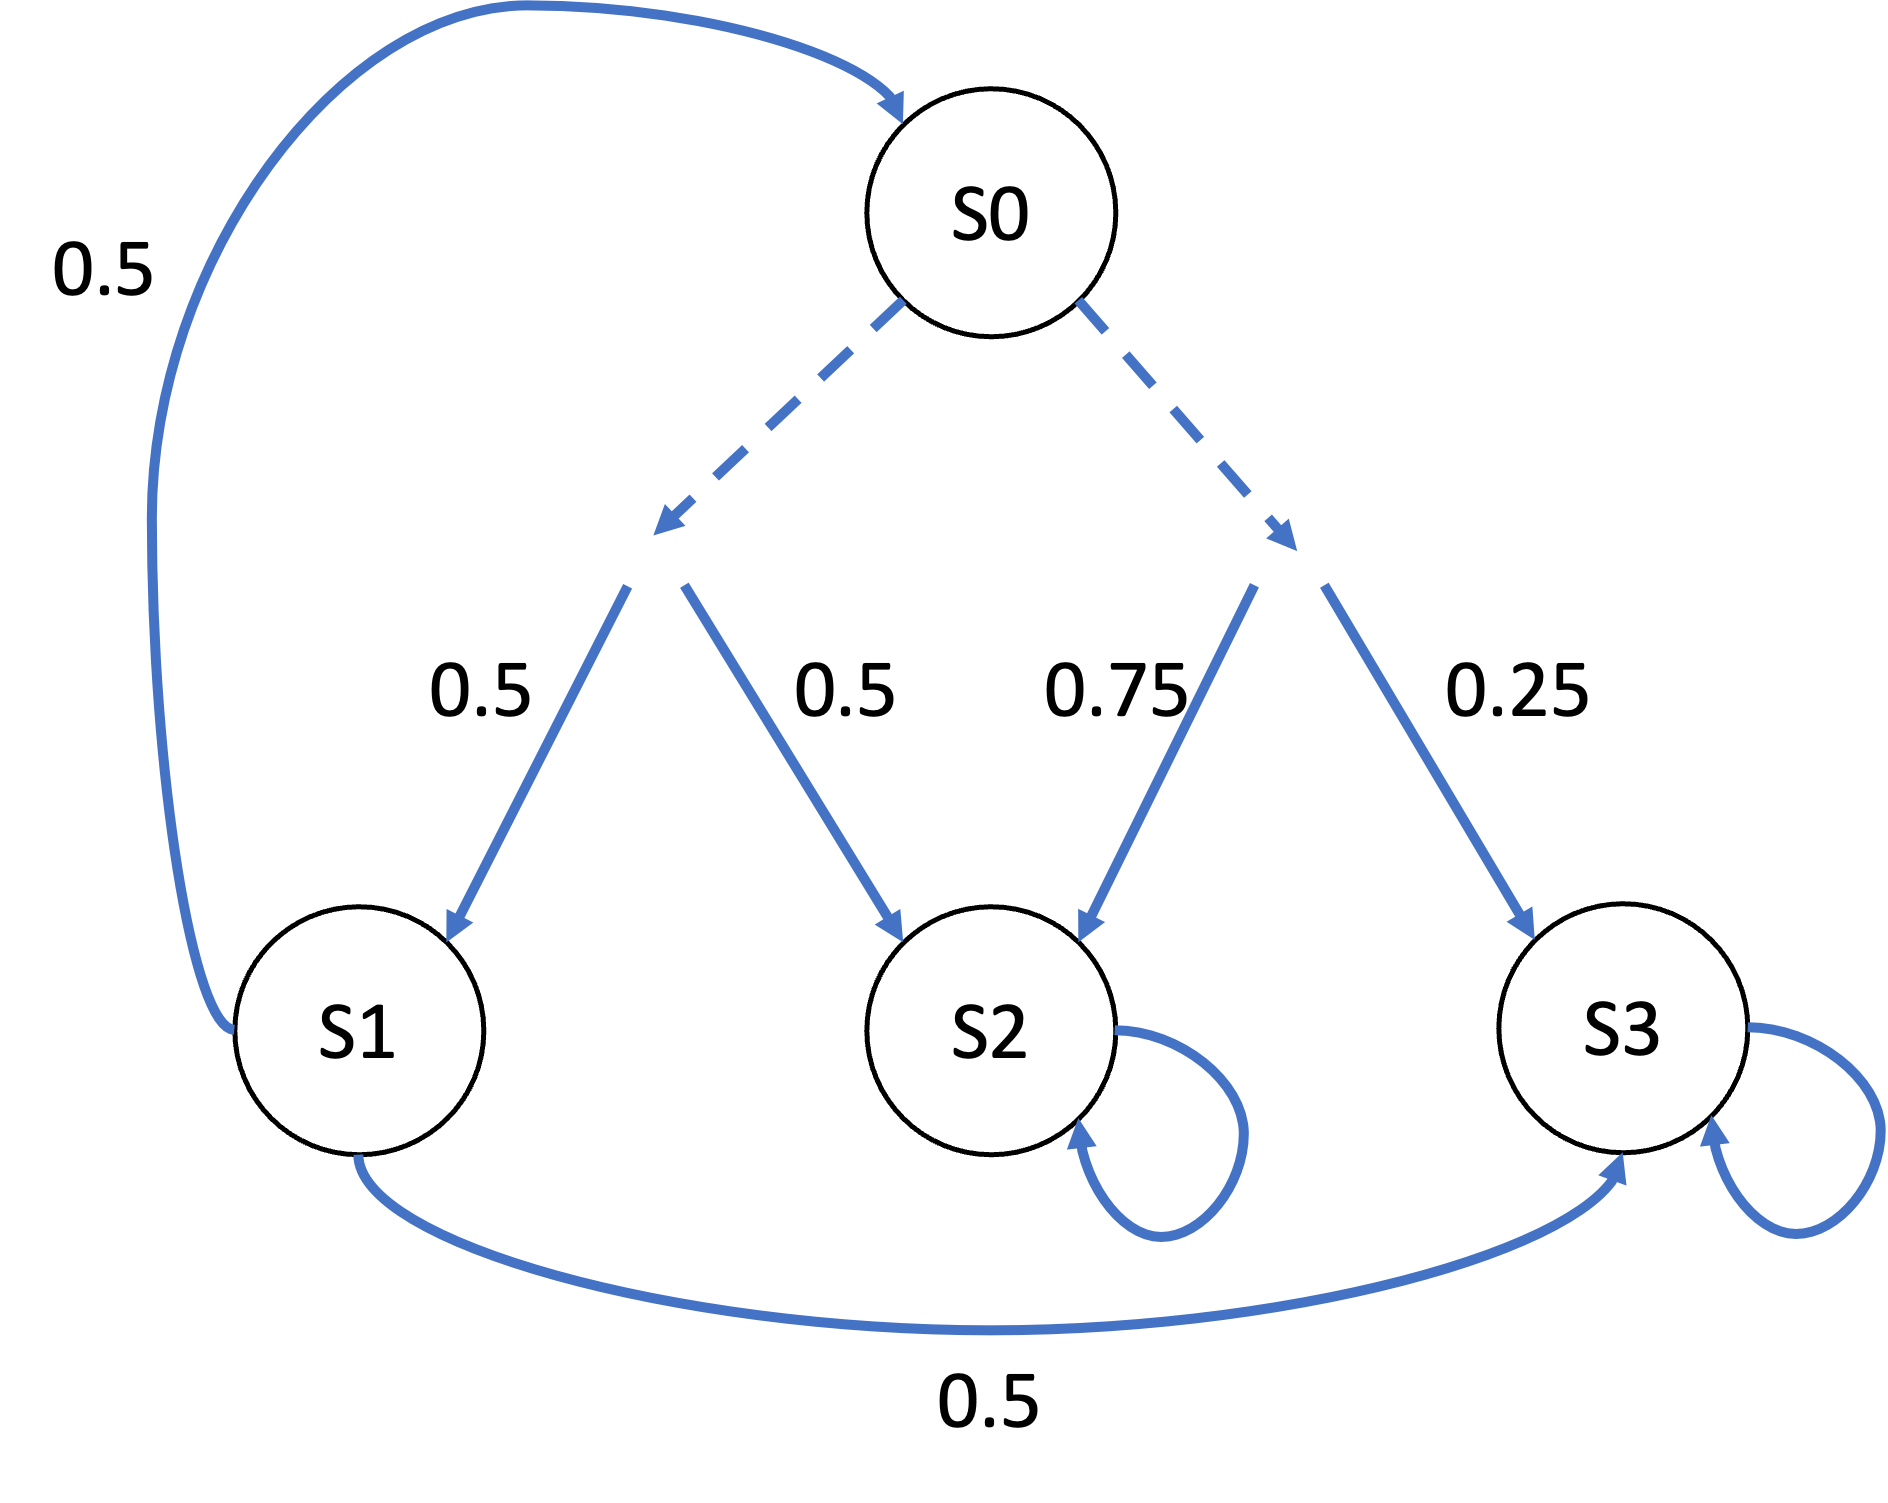
\includegraphics[scale=0.325]{../images/L4_Simple_Pcase_LTD.png} 
            \end{center}
            Let $x_i$ be the max reachability from $S_i$ to $S_2$:
            \begin{itemize}
                \item $x_0 = max(0.5x_1 + 0.5x_2, 0.75x_2 + 0.25x_3)$
                \item $x_1 = 0.5x_0 + 0.5x_3$
                \item $x_2 = 1$
                \item $x_2 = 0$
            \end{itemize}
        \end{column}
        \begin{column}{0.5\textwidth}
            \begin{itemize}
                \item $x_0, x_1$ dependent on other reachability values.
                \item Initially, assume $x_0, x_1 = 0$.
                \item When calculating each current iteration, use the previous iteration's $x_0$ value when calculating $x_1$. That is why in the table below, we start from iteration 0.
                \item Stop iterating only when the values are stabilized.
            \end{itemize}
            \begin{center}
                \begin{scriptsize}
                    \begin{tabular}{|l|l|l|}
                        \hline
                        Iteration & $x_0$ & $x_1$ \\
                        \hline
                        0 & 0 & 0 \\
                        \hline
                        1 & 0.75 & 0 \\
                        \hline
                        2 & 0.75 & 0.375 \\
                        \hline
                        3 & 0.75 & 0.375 \\
                        \hline
                    \end{tabular}
                \end{scriptsize}
            \end{center}
        \end{column}
    \end{columns}
\end{frame}

% Slide 157
\begin{frame}{PCSP Example: Calculating Min Reachability for Simple pcase}
    \begin{columns}
        \begin{column}{0.5\textwidth}
            \begin{center}
                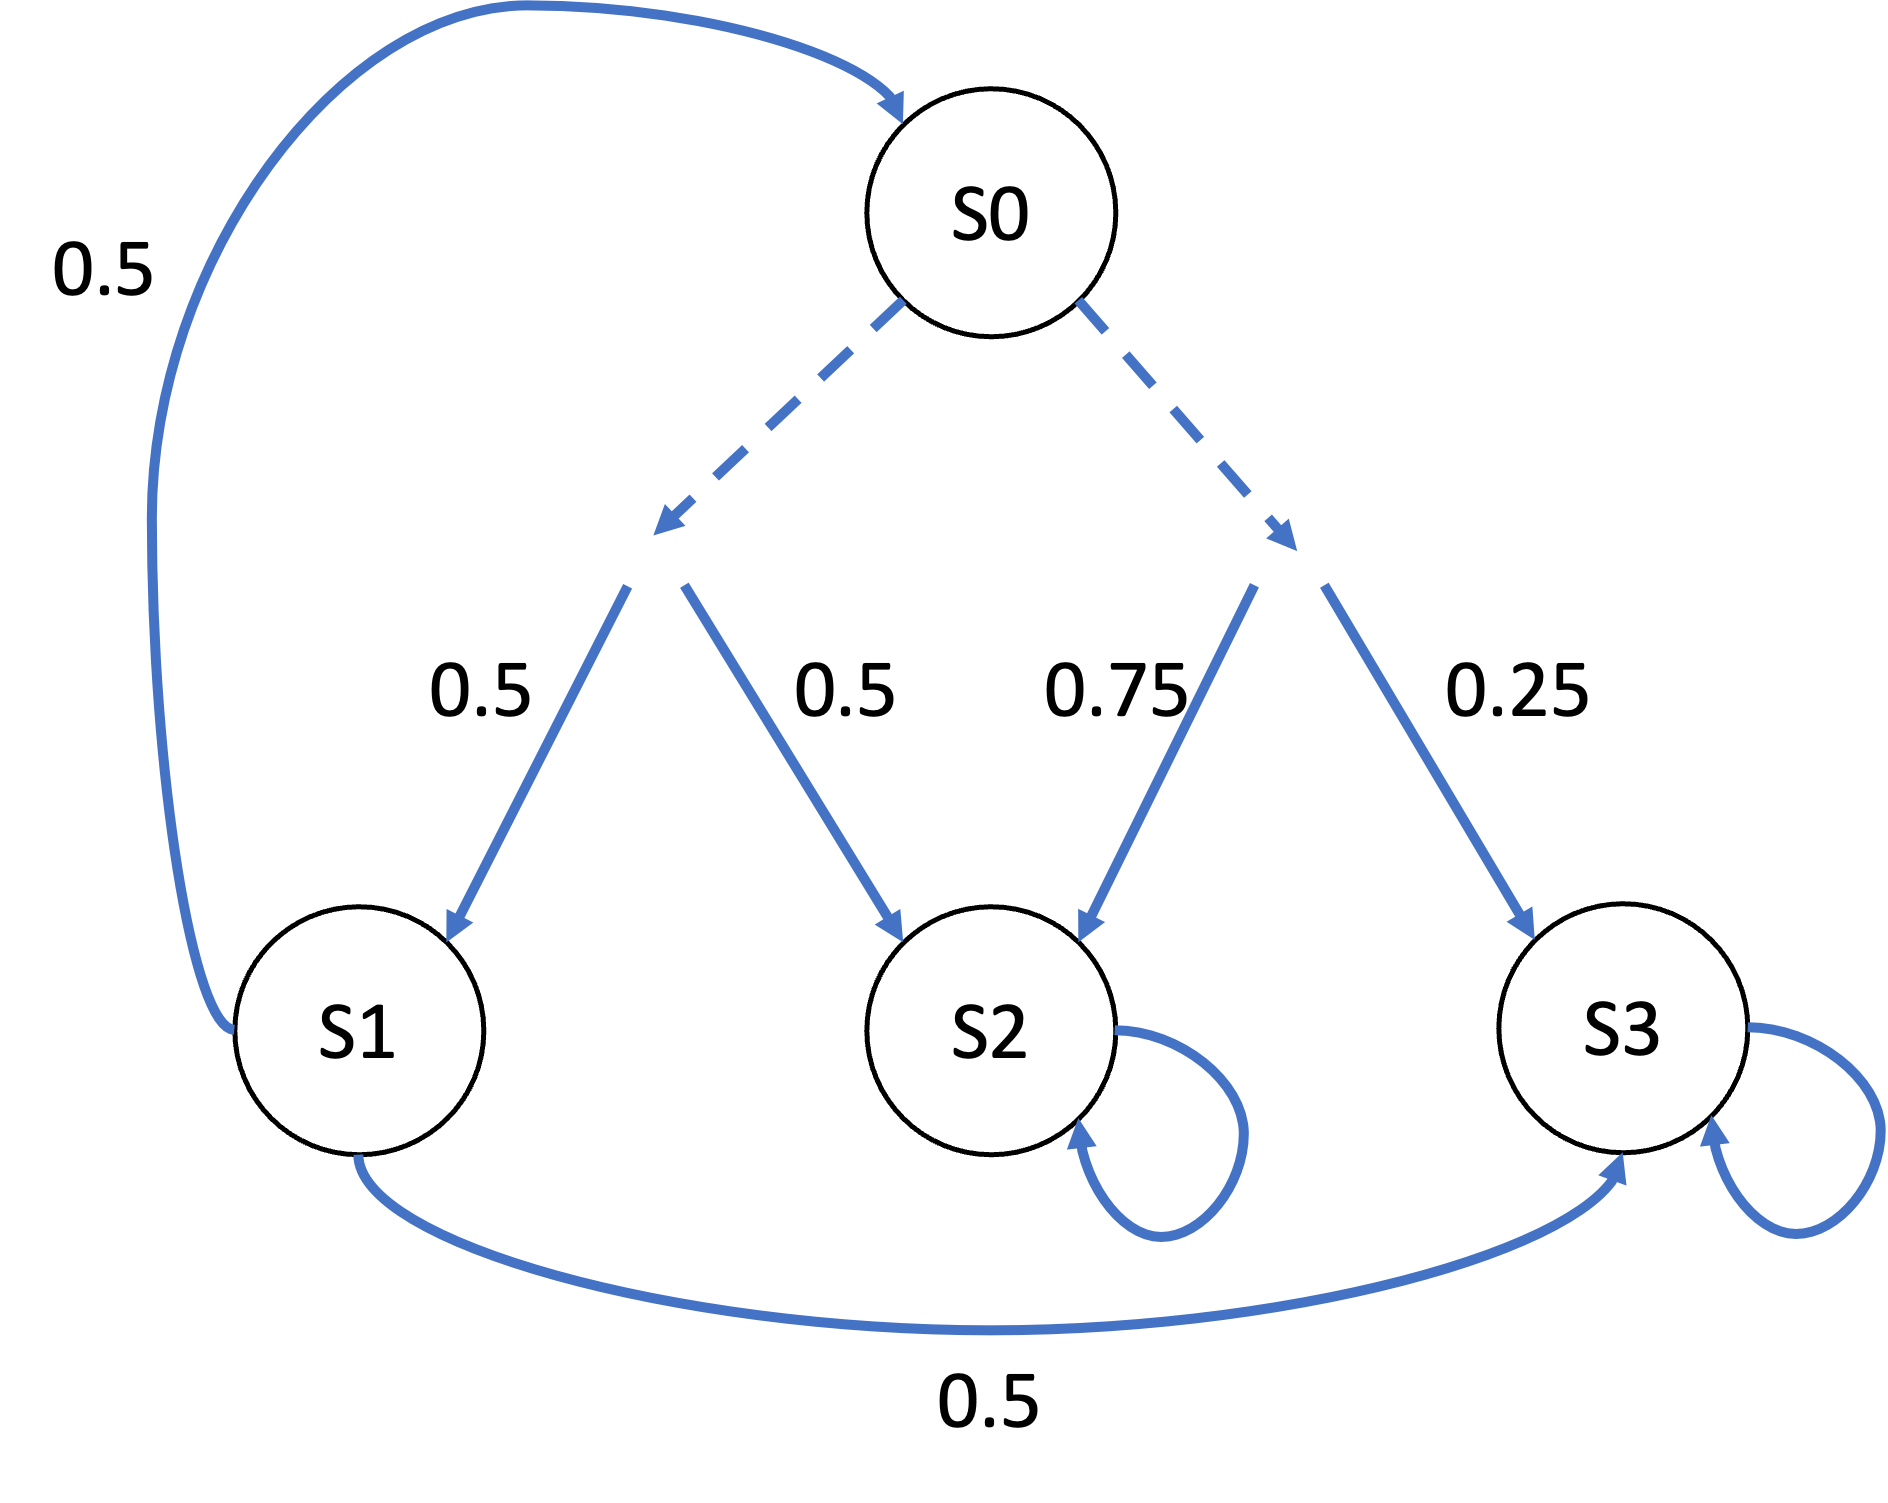
\includegraphics[scale=0.325]{../images/L4_Simple_Pcase_LTD.png} 
            \end{center}
            Let $x_i$ be the min reachability from $S_i$ to $S_2$:
            \begin{itemize}
                \item $x_0 = min(0.5x_1 + 0.5x_2, 0.75x_2 + 0.25x_3)$
                \item $x_1 = 0.5x_0 + 0.5x_3$
                \item $x_2 = 1$
                \item $x_2 = 0$
            \end{itemize}
        \end{column}
        \begin{column}{0.5\textwidth}
            \begin{itemize}
                \item $x_0, x_1$ dependent on other reachability values.
                \item Initially, assume $x_0, x_1 = 1$.
                \item Use the previous iteration's $x_0$ value when calculating $x_1$.
                \item Stop iterating only when the values are stabilized.
            \end{itemize}
            \begin{center}
                \begin{scriptsize}
                    \begin{tabular}{|l|l|l|}
                        \hline
                        Iteration & $x_0$ & $x_1$ \\
                        \hline
                        0 & 1 & 1 \\
                        \hline
                        1 & 0.75 & 0.5 \\
                        \hline
                        2 & 0.75 & 0.375 \\
                        \hline
                        3 & 0.6875 & 0.375 \\
                        \hline
                        4 & 0.6875 & 0.3438 \\
                        \hline
                        5 & 0.6719 & 0.3438 \\
                        \hline
                        $\dots$ &  &  \\
                        \hline
                         & 0.6667 & 0.3333 \\
                        \hline
                    \end{tabular}
                \end{scriptsize}
            \end{center}
        \end{column}
    \end{columns}
\end{frame}

% Slide 158
\begin{frame}[fragile]
\frametitle{PCSP Example: Monty Hall}
\begin{scriptsize}
\begin{lstlisting}[language=C, basicstyle=\scriptsize\selectfont\ttfamily, mathescape]
enum{Door1, Door2, Door3};;
var car = -1;
var guess = -1;
var goat = -1;
var final = false;

#define goal guess == car && final;

PlaceCar = []i:{Door1, Door2, Door3}@ placecar.i{car = i} -> Skip;
Goat = []i:{Door1, Door2, Door3}@ 
    ifb (i != car && i != guess) { hostopen.i{goat = i} -> Skip };

TakeOffer = []i:{Door1, Door2, Door3}@
    ifb (i != guess && i != goat) { changeguess{guess = i; final = true} -> Stop };
NotTakeOffer = keepguess{final = true} -> Stop;

Sys_Take_Offer = PlaceCar; Guest; Goat; TakeOffer;
#assert Sys_Take_Offer reaches goal with prob; // Max Prob = 2/3

Sys_Not_Take_Offer = PlaceCar; Guest; Goat; NotTakeOffer;
#assert Sys_Not_Take_Offer reaches goal with prob; // Max Prob = 1/3

\end{lstlisting}
\end{scriptsize}
\end{frame}

% Slide 159
\begin{frame}[fragile]
\frametitle{PCSP Example: Monty Hall (Explanation)}
\begin{itemize}
    \item What happens if we changed \textbf{line 14} to
\begin{lstlisting}{language=C}
if (i != car && i != guess) { hostopen.i{goat = i} -> Skip };
\end{lstlisting}
    \begin{itemize}
        \item \text{goat} will remain as \texttt{-1}
        \item In the original code, \texttt{ifb} was used. The process will wait at the \texttt{ifb} block when the condition is not true.
        \item However for \texttt{if}, the process will terminate if the condition is not true.
        \item Alternatively, we can change \texttt{ifb} to a guard condition.
    \end{itemize}
    \item The code in the previous slide \textbf{can deadlock}.
    \begin{itemize}
        \item The \texttt{TakeOffer} and \texttt{NotTakeOffer} processes have a \texttt{STOP} process inside its definition.
    \end{itemize}
\end{itemize}
\end{frame}

% Slide 160
\begin{frame}[fragile]
    \frametitle{PCSP Example: Consensus}
\begin{scriptsize}
\begin{lstlisting}[language=C, basicstyle=\scriptsize\selectfont\ttfamily, mathescape]
#define N 2;
#define K 2;
#define range 12; // Range
#define counter_init 6; // Middle
#define left 2; // Left Target
#define right 10; // Right Target
var counter : {0..range} = counter_init; // shared coin
var Pcounter; // record the process number
var coin0counter = N; // number of coints which are 0;
var coin1counter; // number of coints which are 1;
// local variable: 0 - flip, 1 - write, 2 - check, 3 - finished
// processij means this process's coin is i and its local variable is j
process00 = pcase{ [0.5] : process01
                    default : tau {coin0counter--; coin1counter++;} -> process11 };
process01 = [counter > 0] tau {counter--;} -> process02;
process02 = [(counter <= left)] tau {Pcounter++;} -> process03
  [] [(counter >= right)] {Pcounter++; coin0counter--; coin1counter++;} -> process13 
  [] [(counter > left) && (counter < right)] process00;
process03 = [Pcounter==N] done -> process03;
process13 = [Pcounter==N] done -> process13;

System = |||{N}@ process00;
\end{lstlisting}
\end{scriptsize}
\end{frame}

% Slide 161
\begin{frame}{PCSP Example: Consensus (Explanation)}
\begin{itemize}
    \item In this example, $N$ processes come to a consensus by deciding whether the agreed value should be $0$ or $1$.
    \item In \texttt{process00}, there is a $50\%$ chance that the process gets coin 0 in the coin flip which goes to \texttt{process01}. In the remaining $50\%$ chance, the process gets coin 1 in the coin flip and proceeds to \texttt{process11}.
    \item If a process flips coin 0, the counter's value is reduced by 1.
    \item If a process flips coin 1, the counter's value is increased by 1.
    \item If the counter's value is below the left boundary of 2, then the agreed value is 0.
    \item If the counter's value is below the above boundary of 10, then the agreed value is 1.
    \item Note that in this system, all $N$ processes are \textbf{executing concurrently} without synchronisation. Hence, it is possible that the majority decision on the coin value, may differ from the counter value.
    \begin{center}
        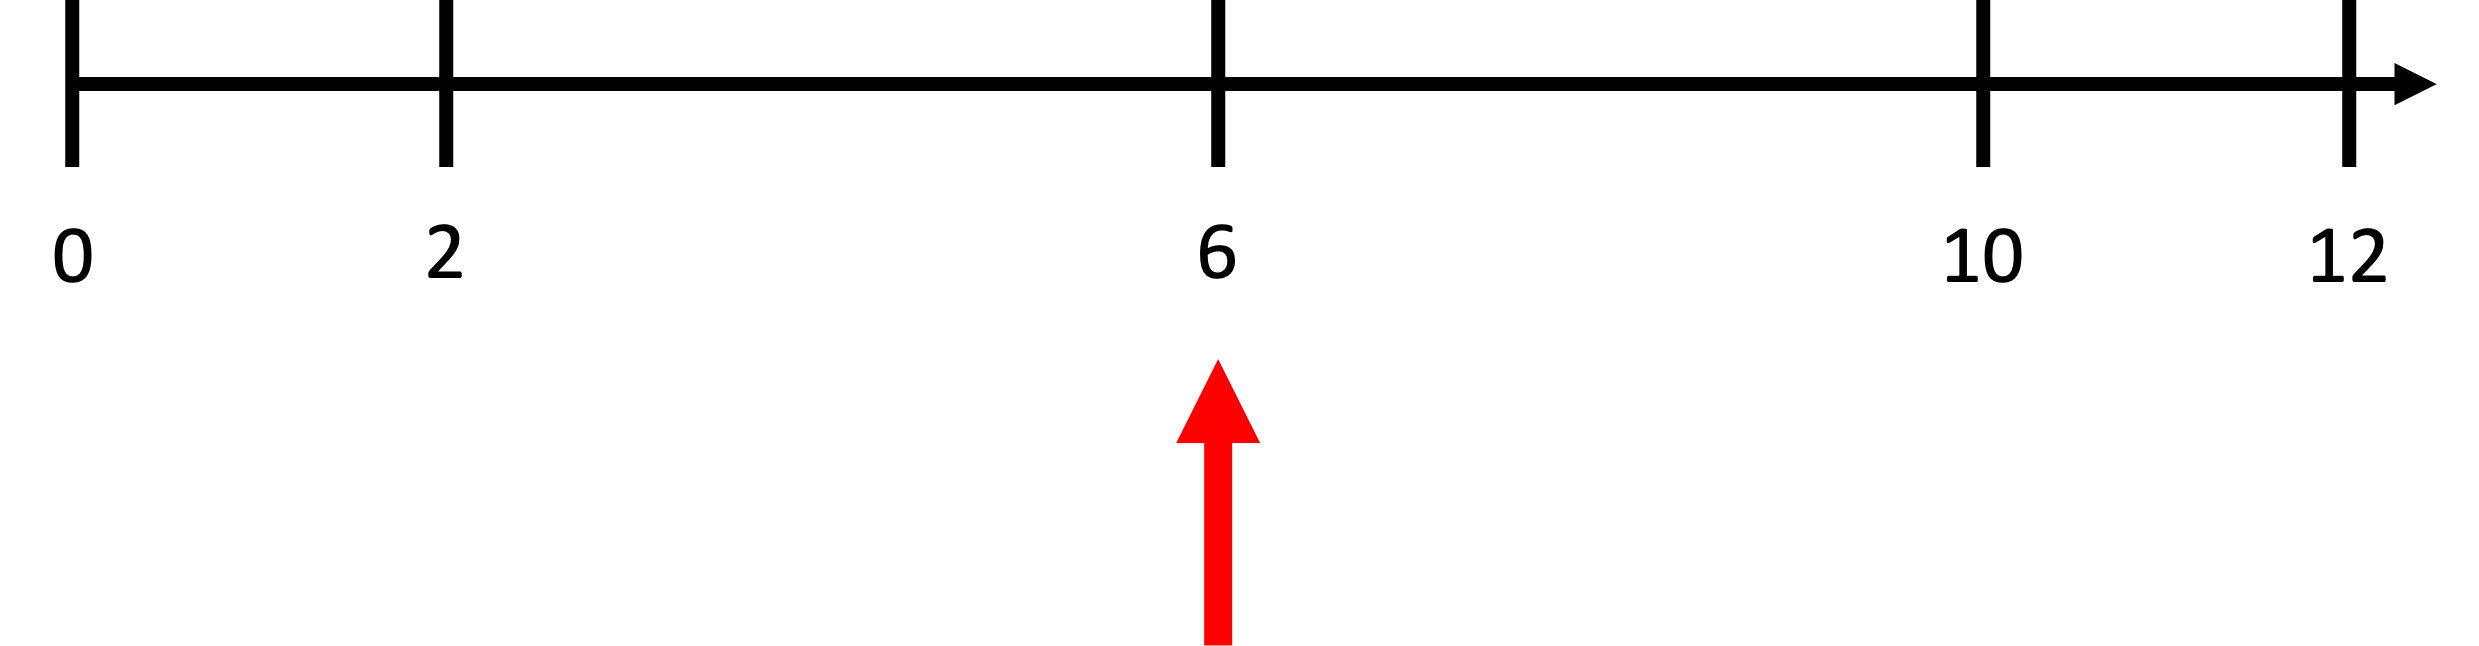
\includegraphics[scale=0.35]{../images/L4Consensus.png}
    \end{center}
\end{itemize}
\end{frame}

% Slide 162
\begin{frame}[fragile]
    \frametitle{PCSP Example: Consensus (Simplified)}
\begin{scriptsize}
\begin{lstlisting}[language=C, basicstyle=\scriptsize\selectfont\ttfamily, mathescape]
#define N 2;
#define K 2;
#define range 12;
#define counter_init 6;
#define left 2;
#define right 6;
var counter: {0..range} = counter_init;
Var Pcounter;

process00 = pcase{ 
    [0.5] : tau{counter--;} -> process02 
     default: tau{counter++;} -> process02
};
process02 = [(counter <= left)] tau{Pcounter++} -> process03;
            [] [(counter >= right)] tau{Pcounter++} -> process13;
            [] [(counter > left) && (counter < right)] process00;
process03 = [Pcounter == N] done -> process03;
Process13 = [Pcounter == N] done -> process13;
System = |||{N}@ process00;    
\end{lstlisting}
\end{scriptsize}
\end{frame}


\end{document}